% To create PDF version, type
%   pdflatex pcasm.tex
% This will produce errors the first time, type R at the error prompt
% Then rerun again (twice to get all the references.

\documentclass[11pt]{book}

%this seems to be more annoying than useful
%\typeout{-----------------------------------------}
%\typeout{Enter files to be included. (*=all)}
%\typeout{(pcasm1,pcasm2,...)}
%\typeout{-----------------------------------------}
%\typein[\infiles]{ }
%\if*\infiles\else\includeonly{\infiles}\fi


\newif\ifmypdf
\ifx\pdfoutput\undefined
    \pdffalse          % we are not running PDFLaTeX
\else
%    \pdfoutput=1       % we are running PDFLaTeX
%    \pdftrue
\fi
%----------------------------------------------------------------------
% The following is the construct that interests us in the end:
%\ifpdf
%   % Put PDF-specific stuff here
%\else
%   % Put LaTeX-specific stuff here
%\fi

\usepackage{indentfirst}  % indent first paragraph of sections
%\usepackage{graphicx}
\usepackage{listings}
\usepackage{epsfig}
\usepackage{longtable}
\usepackage{color}
\usepackage{makeidx}
\usepackage{amsmath}
\usepackage{float}

%\usepackage[pdftitle=PCASM,pdflang=en-US]{hyperref}%accessibility
%\usepackage[tagged]{accessibility}

\usepackage[pdftex,
            bookmarks=true,
            pdflang={en-US},
            pdftitle={PC Assembly Language},
            bookmarksnumbered=true,
            pdfauthor={Paul A. Carter Adapted for SCC's CISP310 by James R. Town},
            pdfsubject={80x86 Assembly Language Programming},
	    pdfkeywords={80x86 assembly programming}]{hyperref}
	 

\hypersetup{
   colorlinks,
    citecolor=black,
    filecolor=black,
    linkcolor=black,
    urlcolor=black
}



\definecolor{blue}{RGB}{0,0,255}
\definecolor{dkgreen}{RGB}{46,133,64}
\definecolor{gray}{rgb}{0.5,0.5,0.5}
\definecolor{mauve}{rgb}{0.58,0,0.82}

   
\author{Paul~A.~Carter \\Adapted for SCC's CISP310 by James R. Town}
\title{PC Assembly Language}
\usepackage{lecnote}
\makeindex


\hyphenation{num-bers SF OF CF DF fact dif-fer-ence inter-rupts op-er-ands}
\begin{document}
\maketitle
\newlength{\AsmMargin}
\setlength{\AsmMargin}{-1cm}
\DefineVerbatimEnvironment{AsmCodeListing}{Verbatim}
{numbers=left, frame=lines,xleftmargin=\AsmMargin, labelposition=all, commentchar=^ }

\newcommand{\MarginNote}[1]{\marginpar{\sloppy \em \small #1}}
\thispagestyle{empty}
\vspace*{\fill}
\noindent This work is licensed under the Creative Commons 
Attribution-NonCommercial-ShareAlike 4.0 International License. To view
a copy of this license, visit
{\code http://creativecommons.org/licenses/by-nc-sa/4.0/}.


\index{subroutine|see{subprogram}}
\index{REPNZ|see{REPNE}}
\index{REPZ|see{REPE}}
\index{C++!member functions|see{methods}}
\index{text segment|see{code segment}}

\vfill
\frontmatter
\tableofcontents

%% -*-LaTex-*-
%front matter of pcasm book

\chapter{Preface}

\section*{Purpose}

The purpose of this book is to give the reader a better understanding
of how computers really work at a lower level than in programming
languages like Pascal. By gaining a deeper understanding of how
computers work, the reader can often be much more productive
developing software in higher level languages such as C and
C++. Learning to program in assembly language is an excellent way to
achieve this goal. Other PC assembly language books still teach how to
program the 8086 processor that the original PC used in 1981!  The
8086 processor only supported \emph{real} mode. In this mode, any
program may address any memory or device in the computer. This mode is
not suitable for a secure, multitasking operating system.  This book
instead discusses how to program the 80386 and later processors in
\emph{protected} mode (the mode that Windows and Linux runs in).
This mode supports the features that modern operating systems expect,
such as virtual memory and memory protection.
There are several reasons to use protected mode:
\begin{enumerate}
\item It is easier to program in protected mode than in the 8086 real mode
      that other books use.
\item All modern PC operating systems run in protected mode.
\item There is free software available that runs in this mode.
\end{enumerate}
The lack of textbooks for protected mode PC assembly programming is the
main reason that the author wrote this book.

Be aware that this text does not attempt to cover every aspect of assembly
programming. The author has tried to cover the most important topics that
\emph{all} programmers should be acquainted with.

\section*{Acknowledgements}

The author would like to thank the many programmers around the world
that have contributed to the Free/Open Source movement. All the
programs and even this book itself were produced using free
software. Specifically, the author would like to thank John~S.~Fine,
Simon~Tatham, Julian~Hall and others for developing the NASM assembler
that all the examples in this book are based on; DJ Delorie for
developing the DJGPP C/C++ compiler used; the numerous people who have
contributed to the GNU gcc compiler on which DJGPP is based on; Donald
Knuth and others for developing the \TeX\ and \LaTeXe\ typesetting
languages that were used to produce the book; Richard Stallman
(founder of the Free Software Foundation), Linus Torvalds (creator of
the Linux kernel) and others who produced the underlying software the
author used to produce this work.

Thanks to the following people for corrections:
\begin{itemize}
\item John S. Fine
\item Marcelo Henrique Pinto de Almeida
\item Sam Hopkins
\item Nick D'Imperio
\item Jeremiah Lawrence
\item Ed Beroset
\item Jerry Gembarowski
\item Ziqiang Peng
\item Eno Compton
\item Josh I Cates
\item Mik Mifflin
\item Luke Wallis
\item Gaku Ueda
\item Brian Heward
\item Chad Gorshing
\item F. Gotti
\item Bob Wilkinson
\item Markus Koegel
\item Louis Taber
\item Dave Kiddell
\item Eduardo Horowitz
\item S\'{e}bastien Le Ray
\item Nehal Mistry
\item Jianyue Wang
\item Jeremias Kleer
\item Marc Janicki
\item Trevor Hansen
\item Giacomo Bruschi
\item Leonardo Rodr\'{i}guez M\'{u}jica
\item Ulrich Bicheler
\item Wu Xing
\item Oleksandr Baranyuk
\end{itemize}


\section*{Resources on the Internet}
\begin{center}
\begin{tabular}{|ll|}
\hline
Author's page & {\code http://pacman128.github.io/} \\
NASM SourceForge page & {\code http://www.nasm.us/} \\
DJGPP  & {\code http://www.delorie.com/djgpp} \\
The Art of Assembly & {\code http://webster.cs.ucr.edu/} \\
USENET & {\code comp.lang.asm.x86 } \\
\hline
\end{tabular}
\end{center}


\section*{Feedback}

The author welcomes any feedback on this work.
\begin{center}
\begin{tabular}{ll}
\textbf{E-mail:} & {\code pacman128@gmail.com} \\
\textbf{WWW:}    & {\code http://pacman128.github.io/pcasm/} \\
\end{tabular}
\end{center}




\mainmatter
% -*-latex-*-
\chapter{Introduction}
\section{Number Systems}

Memory in a computer consists of numbers. Computer memory does not
store these numbers in decimal (base 10). Because it greatly
simplifies the hardware, computers store all information in a binary
(base 2) format. First let's review the decimal system.

\subsection{Decimal\index{decimal}}

Base 10 numbers are composed of 10 possible digits (0-9). Each digit
of a number has a power of 10 associated with it based on its position
in the number. For example:
\begin{displaymath}
234 = 2 \times 10^2 + 3 \times 10^1 + 4 \times 10^0
\end{displaymath}

\subsection{Binary\index{binary|(}}

Base 2 numbers are composed of 2 possible digits (0 and 1). Each digit
of a number has a power of 2 associated with it based on its position
in the number. (A single binary digit is called a bit.) For
example\footnote{The 2 subscript is used to show that the number is
represented in binary, not decimal}:
\begin{eqnarray*}
11001_2 & = & 1 \times 2^4 + 1 \times 2^3 + 0 \times 2^2 + 0 \times 2^1
              + 1 \times 2^0 \\
 & = & 16 + 8 + 1 \\
 & = & 25
\end{eqnarray*}

This shows how binary may be converted to decimal. Table~\ref{tab:dec-bin}
shows how the first few numbers are represented in binary.
\begin{table}[t]
\begin{center}
\begin{tabular}{||c|c||cc||c|c||}
\hline
Decimal & Binary & & & Decimal & Binary \\
\hline
0       & 0000   & & & 8       & 1000 \\
\hline
1       & 0001   & & & 9       & 1001 \\
\hline
2       & 0010   & & & 10      & 1010 \\
\hline
3       & 0011   & & & 11      & 1011 \\
\hline
4       & 0100   & & & 12      & 1100 \\
\hline
5       & 0101   & & & 13      & 1101 \\
\hline
6       & 0110   & & & 14      & 1110 \\
\hline
7       & 0111   & & & 15      & 1111 \\
\hline
\end{tabular}
\caption{Decimal 0 to 15 in Binary\label{tab:dec-bin}}
\end{center}
\end{table}


\begin{figure}[h]
\begin{center}
%I think this example was confusing
%\begin{tabular}{|rrrrrrrrp{.1cm}|p{.1cm}rrrrrrrr|}
%\hline
%& \multicolumn{7}{c}{No previous carry} & & & \multicolumn{7}{c}{Previous carry} & \\
%\hline
%&  0 & &  0 & &  1 & &  1 & & &  0 & &  0 & &  1 & & 1  & \\
%& +0 & & +1 & & +0 & & +1 & & & +0 & & +1 & & +0 & & +1 &  \\
%\cline{2-2} \cline{4-4} \cline{6-6} \cline{8-8} \cline{11-11} \cline{13-13} \cline{15-15} \cline{17-17}
%& 0  & & 1  & & 1  & & 0  & & & 1  & & 0  & & 0  & & 1 & \\
%&    & &    & &    & & c  & & &    & & c  & & c  & & c & \\
%\hline
%\end{tabular}
\begin{tabular}{r}
 $11\overset{1}{0}\overset{1}{1}1_2$ \\
+$10001_2$ \\
\hline
$101100_2$ \\
\end{tabular}

\caption{Binary addition\label{fig:bin-add}}
\index{binary!addition}
\end{center}
\end{figure}

Figure~\ref{fig:bin-add} shows how individual binary digits ({\em
i.e.}, bits) are added. Here's an example:



If one considers the following decimal division:
\[ 1234 \div 10 = 123\; r\; 4 \]
he can see that this division strips off the rightmost decimal digit of
the number and shifts the other decimal digits one position to the right.
Dividing by two performs a similar operation, but for the binary digits
of the number. Consider the following binary division:
\[ 1101_2 \div 10_2 = 110_2\; r\; 1 \]
This fact can be used to convert a decimal
number to its equivalent binary representation as
Figure~\ref{fig:dec-convert} shows. This method finds the rightmost
digit first, this digit is called the \emph{least significant bit} (lsb).
The leftmost digit is called the \emph{most significant bit} (msb).
The basic unit of memory consists of 8 bits and is called a \emph{byte}.
\index{binary|)}

\begin{figure}[t]
%\centering
\fbox{\parbox{\textwidth}{
\begin{center}
\begin{tabular}{cc}
Decimal & Binary \\
$25 \div 2 = 12\;r\;1$ & $11001 \div 10 = 1100\;r\;1$ \\
$12 \div 2 = 6\;r\;0$  & $1100 \div 10 = 110\;r\;0$ \\
$6 \div 2 = 3\;r\;0$   & $110 \div 10 = 11\;r\;0$ \\
$3 \div 2 = 1\;r\;1$   & $11 \div 10 = 1\;r\;1$ \\
$1 \div 2 = 0\;r\;1$   & $1 \div 10 = 0\;r\;1$ \\
\end{tabular}
\end{center}
\centering
Thus $25_{10} = 11001_{2}$
}}
\caption{Decimal conversion to Binary \label{fig:dec-convert}}
\end{figure}

\subsection{Hexadecimal\index{hexadecimal|(}}

Hexadecimal numbers use base 16. Hexadecimal (or \emph{hex} for short) can be
used as a shorthand for binary numbers. Hex has 16 possible
digits. This creates a problem since there are no symbols to use for
these extra digits after 9. By convention, letters are used for these
extra digits. The 16 hex digits are 0-9 then A, B, C, D, E and F. The
digit A is equivalent to 10 in decimal, B is 11, etc. Each digit of a
hex number has a power of 16 associated with it. Example:
\begin{eqnarray*}
\rm
2BD_{16} & = & 2 \times 16^2 + 11 \times 16^1 + 13 \times 16^0 \\
         & = & 512 + 176 + 13 \\
         & = & 701 \\
\end{eqnarray*}
To convert from decimal to hex, use the same idea that was used for
binary conversion except divide by 16. See Figure~\ref{fig:hex-conv} for
an example.

\begin{figure}[t]
\fbox{\parbox{\textwidth}{
\begin{center}
\begin{tabular}{ccc}
$589 \div 16$ & = & $36\;r\;13$ \\
$36 \div 16$ & = & $2\;r\;4$ \\
$2 \div 16$ & = & $0\;r\;2$ \\
\end{tabular}
\end{center}
\centering
Thus $589 = 24\mathrm{D}_{16}$
}}
\caption{Decimal conversion to Hexadecimal \label{fig:hex-conv}}
\end{figure}

The reason that hex is useful is that there is a very simple way to
convert between hex and binary. Binary numbers get large and
cumbersome quickly. Hex provides a much more compact way to represent
binary.

To convert a hex number to binary, simply convert each hex digit to a
4-bit binary number. For example, $\mathrm{24D}_{16}$ is converted to
\mbox{$0010\;0100\; 1101_2$}. Note that the leading zeros of the
4-bits are important! If the leading zero for the middle digit of
$\mathrm{24D}_{16}$ is not used the result is wrong. Converting from
binary to hex is just as easy. One does the process in reverse. Convert
each 4-bit segments of the binary to hex. Start from the
right end, not the left end of the binary number. This ensures that
the process uses the correct 4-bit segments\footnote{If it is not
clear why the starting point makes a difference, try converting the
example starting at the left.}. Example:\newline

\begin{tabular}{cccccc}
$110$ & $0000$ & $0101$ & $1010$ & $0111$ & $1110_2$ \\
  $6$ & $0$    &   $5$  &   A  &  $7$   &    $\mathrm{E}_{16}$ \\
\end{tabular}\newline

A 4-bit number is called a \emph{nibble} \index{nibble}. Thus each hex
digit corresponds to a nibble. Two nibbles make a byte and so a byte
can be represented by a 2-digit hex number. A byte's value ranges from
0 to 11111111 in binary, 0 to FF in hex and 0 to 255 in decimal.
\index{hexadecimal|)}

\subsection{Octal\index{octal|(}}

Octal numbers use base 8. Less common than hexidecimal, octal can also be
used as a shorthand for binary numbers.  It is often used when the numbers
can be broken into groups of three bits.  The first fifteen numbers in octal are shown with their binary equivalents in Table~\ref{tab:oct-bin}.
\begin{table}[t]
\begin{center}
\begin{tabular}{||c|c||cc||c|c||}
\hline
Octal & Binary & & & Octal & Binary \\
\hline
0       & 000   & & & 10       & 001 000 \\
\hline
1       & 001   & & & 11       & 001 001 \\
\hline
2       & 010   & & & 12      & 001 010 \\
\hline
3       & 011   & & & 13      & 001 011 \\
\hline
4       & 100   & & & 14      & 001 100 \\
\hline
5       & 101   & & & 15      & 001 101 \\
\hline
6       & 110   & & & 16      & 001 110 \\
\hline
7       & 111   & & & 17      & 001 111 \\
\hline
\end{tabular}
\caption{Octal 0 to 17 in Binary\label{tab:oct-bin}}
\end{center}
\end{table}

\index{octal|)}

\section{Computer Organization}

\subsection{Memory\index{memory|(}}

The basic unit of memory is a byte. \index{byte} \MarginNote{Memory is
measured in units of kilobytes (~$2^{10} = 1,024$ bytes), megabytes
(~$2^{20} = 1,048,576$ bytes) and gigabytes (~$2^{30} = 1,073,741,824$
bytes).}A computer with 32 megabytes of memory can hold roughly 32
million bytes of information. Each byte in memory is labeled by a
unique number known as its address as Figure~\ref{fig:memory} shows.

\begin{figure}[ht]
\begin{center}
\begin{tabular}{rcccccccc}
Address & 0 & 1 & 2 & 3 & 4 & 5 & 6 & 7 \\
\cline{2-9}
Memory & \multicolumn{1}{|c}{2A}  & \multicolumn{1}{|c}{45}
       & \multicolumn{1}{|c}{B8} & \multicolumn{1}{|c}{20}
       & \multicolumn{1}{|c}{8F} & \multicolumn{1}{|c}{CD}
       & \multicolumn{1}{|c}{12} & \multicolumn{1}{|c|}{2E} \\
\cline{2-9}
\end{tabular}
\caption{ Memory Addresses \label{fig:memory} }
\end{center}
\end{figure}

\begin{table}[t]
\begin{center}
\begin{tabular}{|l|l|}
\hline
Term & Size \\ \hline
nibble & 1/2 bytes \\ \hline
byte & 1 byte \\ \hline
word & 2 bytes \\ \hline
double word & 4 bytes \\ \hline
quad word & 8 bytes \\ \hline
paragraph & 16 bytes \\ \hline
\end{tabular}
\caption{ Units of Memory \label{tab:mem_units} }
\end{center}
\end{table}

Often memory is used in larger chunks than single bytes. On
the PC architecture, names have been given to these larger sections of
memory as Table~\ref{tab:mem_units} shows.

All data in memory is numeric. Characters are stored by using a
\emph{character code} that maps numbers to characters. One of the
most common character codes is known as \emph{ASCII} (American
Standard Code for Information Interchange). A new, more complete code
that is supplanting ASCII is Unicode. One key difference between the
two codes is that ASCII uses one byte to encode a character, but
Unicode uses multiple bytes. There are several different forms of Unicode.
On x86 C/C++ compilers, Unicode is represented in code using the
{\code wchar\_t} type and the UTF-16 encoding which uses 16 bits (or a
\emph{word}) per character. For example, ASCII maps the byte $41_{16}$
($65_{10}$) to the character capital \emph{A}; UTF-16 maps it to the
word $0041_{16}$. Since ASCII uses a byte, it is limited to only 256
different characters\footnote{In fact, ASCII only uses the lower 7-bits
and so only has 128 different values to use.}. Unicode extends the ASCII
values and allows many more characters to be represented. This is important
for representing characters for all the languages of the world.
\index{memory|)}

\subsection{The CPU\index{CPU|(}}

The Central Processing Unit (CPU) is the physical device that performs
instructions. The instructions that CPUs perform are generally very
simple. Instructions may require the data they act on to be in special
storage locations in the CPU itself called
\emph{registers}. \index{register} The CPU can access data in registers
much faster than data in memory. However, the number of registers in a
CPU is limited, so the programmer must take care to keep only
currently used data in registers.

The instructions a type of CPU executes make up the CPU's
\emph{machine language}. \index{machine language} Machine programs
have a much more basic structure than higher-level languages. Machine
language instructions are encoded as raw numbers, not in friendly text
formats. A CPU must be able to decode an instruction's purpose very
quickly to run efficiently. Machine language is designed with this
goal in mind, not to be easily deciphered by humans. Programs written
in other languages must be converted to the native machine language of
the CPU to run on the computer. A \emph{compiler} \index{compiler} is
a program that translates programs written in a programming language
into the machine language of a particular computer architecture. In
general, every type of CPU has its own unique machine language. This
is one reason why programs written for a Mac can not run on an
IBM-type PC.

Computers use a \emph{clock} \index{clock} to synchronize the
execution of the \MarginNote{\emph{GHz} stands for gigahertz or one
billion cycles per second.  A 1.5 GHz CPU has 1.5 billion clock pulses
per second.} instructions.  The clock pulses at a fixed frequency
(known as the \emph{clock speed}). When you buy a 1.5 GHz computer,
1.5 GHz is the frequency of this clock\footnote{Actually, clock pulses
are used in many different components of a computer. The other
components often use different clock speeds than the CPU.}. The clock
does not keep track of minutes and seconds. It simply beats at a
constant rate. The electronics of the CPU uses the beats to perform
their operations correctly, like how the beats of a metronome help one
play music at the correct rhythm.  The number of beats (or as they are
usually called \emph{cycles}) an instruction requires depends on the
CPU generation and model. The number of cycles depends on the
instructions before it and other factors as well.


\subsection{The 80x86 family of CPUs\index{CPU!80x86}}

IBM-type PC's contain a CPU from Intel's 80x86 family (or a clone of one).
The CPU's in this family all have some common features including a base
machine language. However, the more recent members greatly enhance the
features.
\begin{description}

\item[8088,8086:] These CPU's from the programming standpoint are
identical. They were the CPU's used in the earliest PC's. They provide
several 16-bit registers: AX, BX, CX, DX, SI, DI, BP, SP, CS, DS, SS,
ES, IP, FLAGS. They only support up to one megabyte of memory and only
operate in \emph{real mode}.  In this mode, a program may access any
memory address, even the memory of other programs! This makes
debugging and security very difficult! Also, program memory has to be
divided into \emph{segments}. Each segment can not be larger than
64K.

\item[80286:] This CPU was used in AT class PC's. It adds some new
instructions to the base machine language of the 8088/86.  However,
its main new feature is \emph{16-bit protected mode}.  In this mode,
it can access up to 16 megabytes and protect programs from accessing
each other's memory. However, programs are still divided into
segments that could not be bigger than 64K.

\item[80386:] This CPU greatly enhanced the 80286. First, it extends many
of the registers to hold 32-bits (EAX, EBX, ECX, EDX, ESI, EDI, EBP, ESP,
EIP) and adds two new 16-bit registers FS and GS. It also adds a new
\emph{32-bit protected mode}. In this mode, it can access up to 4 gigabytes.
Programs are again divided into segments, but now each segment can also be
up to 4 gigabytes in size!

\item[80486/Pentium/Pentium Pro:] These members of the 80x86 family add
very few new features. They mainly speed up the execution of the
instructions.

\item[Pentium MMX:] This processor adds the MMX (MultiMedia eXtensions)
instructions to the Pentium. These instructions can speed up common graphics
operations.

\item[Pentium II:] This is the Pentium Pro processor with the MMX instructions
added. (The Pentium III is essentially just a faster Pentium II.)

\end{description}
\index{CPU|)}

\subsection{8086 16-bit Registers\index{register|(}}

The original 8086 CPU provided four 16-bit general purpose registers:
AX, BX, CX and DX. Each of these registers could be decomposed into
two 8-bit registers. For example, the AX register could be decomposed
into the AH and AL registers as Figure~\ref{fig:AX_reg} shows. The AH
register contains the upper (or high) 8 bits of AX and AL contains the
lower 8 bits of AX. Often AH and AL are used as independent one byte
registers; however, it is important to realize that they are not
independent of AX. Changing AX's value will change AH and AL and
{\em vice versa}\/. The general purpose registers are used in many of
the data movement and arithmetic instructions.

\begin{figure}
\begin{center}
\begin{tabular}{cc}
\multicolumn{2}{c}{AX} \\
\hline
\multicolumn{1}{||c|}{AH} & \multicolumn{1}{c||}{AL} \\
\hline
\end{tabular}
\caption{The AX register \label{fig:AX_reg} }
\end{center}
\end{figure}

There are two 16-bit index registers\index{register!index}: SI and
DI. They are often used as pointers, but can be used for many of the
same purposes as the general registers. However, they can not be
decomposed into 8-bit registers.

The 16-bit BP and SP registers are used to point to data in the
machine language stack and are called the Base Pointer\index{register!base pointer}
and Stack Pointer\index{register!stack pointer}, respectively. These will be discussed later.

The 16-bit CS, DS, SS and ES registers are \emph{segment
registers}. \index{register!segment} They denote what memory is used
for different parts of a program. CS stands for Code Segment, DS for
Data Segment, SS for Stack Segment and ES for Extra Segment. ES is
used as a temporary segment register. The details of these registers
are in Sections~\ref{real_mode} and \ref{16prot_mode}.

The Instruction Pointer (IP) \index{register!IP} register is used with
the CS register to keep track of the address of the next instruction
to be executed by the CPU. Normally, as an instruction is executed, IP
is advanced to point to the next instruction in memory.

The FLAGS \index{register!FLAGS} register stores important information
about the results of a previous instruction. These results are stored
as individual bits in the register. For example, the Z bit is 1 if the
result of the previous instruction was zero or 0 if not zero. Not all
instructions modify the bits in FLAGS, consult the table in the
appendix to see how individual instructions affect the FLAGS register.

\subsection{80386 32-bit registers\index{register!32-bit}}

The 80386 and later processors have extended registers. For example, the
16-bit AX register is extended to be 32-bits. To be backward compatible, AX
still refers to the 16-bit register and EAX is used to refer to the extended
32-bit register. AX is the lower 16-bits of EAX just as AL is the lower 8-bits
of AX (and EAX). There is no way to access the upper 16-bits of EAX directly.
The other extended registers are EBX, ECX, EDX, ESI and EDI.

Many of the other registers are extended as well. BP becomes
EBP\index{register!base pointer}; SP becomes ESP\index{register!stack
pointer}; FLAGS becomes EFLAGS\index{register!EFLAGS} and IP becomes
EIP\index{register!EIP}. However, unlike the index and general purpose
registers, in 32-bit protected mode (discussed below) only the
extended versions of these registers are used.

The segment registers are still 16-bit in the 80386. There are also
two new segment registers: FS and GS\index{register!segment}. Their
names do not stand for anything. They are extra temporary segment
registers (like ES).

One of definitions of the term \emph{word} \index{word} refers to the
size of the data registers of the CPU. For the 80x86 family, the term
is now a little confusing. In Table~\ref{tab:mem_units}, one sees that
\emph{word} is defined to be 2 bytes (or 16 bits). It was given this
meaning when the 8086 was first released. When the 80386 was
developed, it was decided to leave the definition of \emph{word}
unchanged, even though the register size changed.
\index{register|)}

\subsection{Real Mode \label{real_mode} \index{real mode|(}}

In \MarginNote{So where did the infamous DOS 640K limit come from? The BIOS
required some of the 1M for its code and for hardware devices like the video
screen.} real mode, memory is limited to only one megabyte ($2^{20}$ bytes).
Valid
address range from (in hex) 00000 to FFFFF.\@  % \@ means end of sentence
These addresses require a 20-bit number. Obviously, a 20-bit number will not
fit into any of the 8086's 16-bit registers. Intel solved this problem, by
using two 16-bit values to determine an address. The first 16-bit value is called
the \emph{selector}. Selector values must be stored in segment registers. The
second 16-bit value is called the \emph{offset}. The physical address
referenced by a 32-bit \emph{selector:offset} pair is computed by the formula
\[ 16 * {\rm selector} + {\rm offset} \]
Multiplying by 16 in hex is easy, just add a 0 to the right of the number. For
example, the physical addresses referenced by 047C:0048 is given by:
\begin{center}
\begin{tabular}{r}
047C0 \\
+0048 \\
\hline
04808 \\
\end{tabular}
\end{center}
In effect, the selector value is a paragraph number
(see Table~\ref{tab:mem_units}).

Real segmented addresses have disadvantages:
\begin{itemize}
\item A single selector value can only reference 64K of memory (the
upper limit of the 16-bit offset). What if a program has more than 64K
of code? A single value in CS can not be used for the entire execution
of the program.  The program must be split up into sections (called
\emph{segments}\index{memory!segments}) less than 64K in size. When
execution moves from one segment to another, the value of CS must be
changed. Similar problems occur with large amounts of data and the DS
register. This can be very awkward!

\item Each byte in memory does not have a unique segmented address. The
physical address 04808 can be referenced by 047C:0048, 047D:0038, 047E:0028
or 047B:0058.\@ This can complicate the comparison of segmented addresses.

\end{itemize}
\index{real mode|)}

\subsection{16-bit Protected Mode \label{16prot_mode} \index{protected mode!16-bit|(}}

In the 80286's 16-bit protected mode, selector values are interpreted
completely differently than in real mode. In real mode, a selector
value is a paragraph number of physical memory. In protected mode, a
selector value is an \emph{index} into a \emph{descriptor table}. In
both modes, programs are divided into
segments\index{memory:segments}. In real mode, these segments are at
fixed positions in physical memory and the selector value denotes the
paragraph number of the beginning of the segment. In protected mode,
the segments are not at fixed positions in physical memory. In fact,
they do not have to be in memory at all!

Protected mode uses a technique called \emph{virtual memory}
\index{memory!virtual}. The basic idea of a virtual memory system is
to only keep the data and code in memory that programs are currently
using. Other data and code are stored temporarily on disk until they
are needed again.  In 16-bit protected mode, segments are moved
between memory and disk as needed. When a segment is returned to
memory from disk, it is very likely that it will be put into a
different area of memory that it was in before being moved to
disk. All of this is done transparently by the operating system. The
program does not have to be written differently for virtual memory to
work.

In protected mode, each segment is assigned an entry in a descriptor table.
This entry has all the information that the system needs to know about the
segment. This information includes: is it currently in memory; if in memory,
where is it; access permissions ({\em e.g.\/}, read-only). The index of the
entry of the segment is the selector value that is stored in segment registers.

One \MarginNote{One well-known PC columnist called the 286 CPU ``brain
dead.''} big disadvantage of 16-bit protected mode is that offsets
are still 16-bit quantities. As a consequence of this, segment sizes
are still limited to at most 64K. This makes the use of large arrays
problematic!
\index{protected mode!16-bit|)}

\subsection{32-bit Protected Mode\index{protected mode!32-bit|(}}

The 80386 introduced 32-bit protected mode. There are two major differences
between 386 32-bit and 286 16-bit protected modes:
\begin{enumerate}
\item

Offsets are expanded to be 32-bits. This allows an offset to range up
to 4 billion. Thus, segments can have sizes up to 4 gigabytes.

\item

Segments\index{memory!segments} can be divided into smaller 4K-sized
units called \emph{pages}\index{memory!pages}. The virtual
memory\index{memory!virtual} system works with pages now instead of
segments. This means that only parts of segment may be in memory at
any one time. In 286 16-bit mode, either the entire segment is in
memory or none of it is. This is not practical with the larger
segments that 32-bit mode allows.

\end{enumerate}

\index{protected mode!32-bit|)}

In Windows 3.x, \emph{standard mode} referred to 286 16-bit protected mode and
\emph{enhanced mode} referred to 32-bit mode. Windows 9X, Windows NT/2000/XP, OS/2
and Linux all run in paged 32-bit protected mode.

\subsection{Interrupts\index{interrupt}}

Sometimes the ordinary flow of a program must be interrupted to process events
that require prompt response. The hardware of a computer provides a mechanism
called \emph{interrupts} to handle these events. For example, when a mouse is
moved, the mouse hardware interrupts the current program to handle the mouse
movement (to move the mouse cursor, {\em etc.\/}) Interrupts cause control to
be passed to an \emph{interrupt handler}. Interrupt handlers are routines that
process the interrupt. Each type of interrupt is assigned an integer number.
At the beginning of physical memory, a table of \emph{interrupt vectors}
resides that contain the segmented addresses of the interrupt handlers. The
number of interrupt is essentially an index into this table.

External interrupts are raised from outside the CPU. (The mouse is an
example of this type.) Many I/O devices raise interrupts ({\em
e.g.\/}, keyboard, timer, disk drives, CD-ROM and sound
cards). Internal interrupts are raised from within the CPU, either
from an error or the interrupt instruction. Error interrupts are also
called \emph{traps}. Interrupts generated from the interrupt
instruction are called \emph{software interrupts}. DOS uses these types of
interrupts to implement its API (Application Programming Interface). More
modern operating systems (such as Windows and UNIX) use a C based interface.
\footnote{However, they may use a lower level interface at the kernel level.}

Many interrupt handlers return control back to the interrupted program
when they finish. They restore all the registers to the same values
they had before the interrupt occurred. Thus, the interrupted program
runs as if nothing happened (except that it lost some CPU
cycles). Traps generally do not return. Often they abort the program.

\section{Assembly Language}

\subsection{Machine language\index{machine language}}

Every type of CPU understands its own machine language. Instructions
in machine language are numbers stored as bytes in memory. Each
instruction has its own unique numeric code called its \emph{operation
code} or \emph{opcode} \index{opcode} for short. The 80x86 processor's
instructions vary in size.  The opcode is always at the beginning of
the instruction. Many instructions also include data ({\em e.g.\/},
constants or addresses) used by the instruction.

Machine language is very difficult to program in directly. Deciphering the
meanings of the numerical-coded instructions is tedious for humans. For
example, the instruction that says to add the EAX and EBX registers together
and store the result back into EAX is encoded by the following hex codes:
\begin{quote}
   03 C3
\end{quote}
This is hardly obvious. Fortunately, a program called an
\emph{assembler} \index{assembler} can do this tedious work for the
programmer.

\subsection{Assembly language\index{assembly language|(}}

An assembly language program is stored as text (just as a higher level language
program). Each assembly instruction represents exactly one machine instruction.
For example, the addition instruction described above would be represented
in assembly language as:
\begin{CodeQuote}
   add eax, ebx
\end{CodeQuote}
Here the meaning of the instruction is \emph{much} clearer than in
machine code. The word {\code add} is a \emph{mnemonic}
\index{mnemonic} for the addition instruction.  The general form of an
assembly instruction is:
\begin{CodeQuote}
  {\em mnemonic operand(s)}
\end{CodeQuote}

An \emph{assembler} \index{assembler} is a program that reads a text
file with assembly instructions and converts the assembly into machine
code.  \emph{Compilers} \index{compiler} are programs that do similar
conversions for high-level programming languages. An assembler is much
simpler than a compiler. \MarginNote{It took several years for
computer scientists to figure out how to even write a compiler!} Every
assembly language statement directly represents a single machine
instruction. High-level language statements are \emph{much} more
complex and may require many machine instructions.

Another important difference between assembly and high-level languages is that
since every different type of CPU has its own machine language, it also has
its own assembly language. Porting assembly programs between different computer
architectures is \emph{much} more difficult than in a high-level language.

This book's examples uses the Microsoft's Assembler or MASM \index{MASM}
for short. It is freely available off the Internet. More common assemblers are Netwide Assembler (NASM)
\index{NASM} or Borland's Assembler (TASM). \index{TASM} There are
some differences in the assembly syntax for MASM/TASM and NASM, but the
big ideas are the same.

\subsection{Instruction operands}

Machine code instructions have varying number and type of operands; however,
in general, each instruction itself will have a fixed number of operands (0
to 3). Operands can have the following types:
\begin{description}
\item[register:]
These operands refer directly to the contents of the CPU's registers.
\item[memory:]
These refer to data in memory. The address of the data may be a constant
hardcoded into the instruction or may be computed using values of registers.
Address are always offsets from the beginning of a segment.
\item[immediate:]
\index{immediate}
These are fixed values that are listed in the instruction itself. They are
stored in the instruction itself (in the code segment), not in the data
segment.
\item[implied:]
These operands are not explicitly shown. For example, the increment
instruction adds one to a register or memory. The one is implied.
\end{description}
\index{assembly language|)}

\subsection{Basic instructions}

The most basic instruction is the {\code MOV} \index{MOV} instruction. It moves
data from one location to another (like the assignment operator in a
high-level language). It takes two operands:
\begin{CodeQuote}
  mov {\em dest, src}
\end{CodeQuote}
The data specified by {\em src} is copied to {\em dest\/}. One restriction
is that both operands may not be memory operands. This points out another
quirk of assembly. There are often somewhat arbitrary rules about how the
various instructions are used. The operands must also be the same size. The
value of AX can not be stored into BL.

\lstset{%frame=tb,
   language=[x86masm]Assembler,
   morekeywords={.code},
   aboveskip=3mm,
   belowskip=3mm,
   showstringspaces=false,
   columns=flexible,
   basicstyle={\small\ttfamily},
   numbers=left,%none,%
   numberstyle=\tiny\color{gray},
   keywordstyle=\color{blue},
   commentstyle=\color{dkgreen},
   stringstyle=\color{mauve},
   breaklines=true,
   frame=none,
   breakatwhitespace=true,
   tabsize=3
   }

Here is an example (semicolons start a comment\index{comment}):
%\begin{AsmCodeListing}[frame=none, numbers=none]
\begin{lstlisting}[language={[x86masm]Assembler}]
  mov    eax, 3   ; store 3 into EAX register (3 is immediate operand)
  mov    bx, ax   ; store the value of AX into the BX register
\end{lstlisting}
%AsmCodeListing}

The {\code ADD} \index{ADD} instruction is used to add integers.
\begin{lstlisting}[language={[x86masm]Assembler}]
  add    eax, 4   ; eax = eax + 4
  add    al, ah   ; al = al + ah
\end{lstlisting}

The {\code SUB} \index{SUB} instruction subtracts integers.
\begin{lstlisting}[language={[x86masm]Assembler}]
  sub    bx, 10   ; bx = bx - 10
  sub    ebx, edi ; ebx = ebx - edi
\end{lstlisting}

The {\code INC} \index{INC} and {\code DEC} \index{DEC} instructions
increment or decrement values by one. Since the one is an implicit
operand, the machine code for {\code INC} and {\code DEC} is smaller
than for the equivalent {\code ADD} and {\code SUB} instructions.
\begin{lstlisting}[language={[x86masm]Assembler}]
  inc    ecx      ; ecx++
  dec    dl       ; dl--
\end{lstlisting}

\subsection{Directives\index{directive|(}}

A \emph{directive} is an artifact of the assembler not the CPU. They are
generally used to either instruct the assembler to do something or inform
the assembler of something. They are not translated into machine code. Common
uses of directives are:
\begin{list}{$\bullet$}{\setlength{\itemsep}{0pt}}
\item define constants
\item define memory to store data into
\item group memory into segments
\item conditionally include source code
\item include other files
\end{list}

\subsubsection{The equ directive\index{directive!equ}}

The {\code equ} directive can be used to define a \emph{symbol}. Symbols are
named constants that can be used in the assembly program. The format is:
\begin{quote}
  \code {\em symbol} equ {\em value}
\end{quote}
Symbol values can \emph{not} be redefined later.

\subsubsection{Data directives\index{directive!data|(}}

\begin{table}[t]
\centering
\begin{tabular}{||c|c||} \hline
{\bf Unit} & {\bf Letter} \\
\hline
byte & B \\
word & W \\
double word & D \\
quad word & Q \\
ten bytes & T \\
\hline
\end{tabular}
\caption{Letters for {\code DX} Directives
         \label{tab:size-letters} }
\end{table}

Data directives are used in data segments to define room for
memory. There are two ways memory can be reserved. The first way only
defines room for data; the second way defines room and an initial
value. You can use a ? to reserve uninitialized memory for a given size,
or you can give the memory location an initial value.
%The first method uses one of the {\code RES{\em
%X}}\index{directive!RES\emph{X}} directives. The {\em X} is replaced
%with a letter that determines the size of the object (or objects) that
%will be stored.
Table~\ref{tab:size-letters} shows the possible
values for the different sizes of data.

%The second method (that defines an initial value, too) uses one of the
%{\code D{\em X}} directives\index{directive!D\emph{X}}. The {\em X}
%letters are the same as those in the {\code RES{\em X}} directives.


It is very common to mark memory locations with
\emph{labels}. \index{label} Labels allow one to easily refer to
memory locations in code. Below are several examples:
\begin{lstlisting}[language={[x86masm]Assembler}]
L1  db  0        ; byte labeled L1 with initial value 0
L2  dw  1000     ; word labeled L2 with initial value 1000
L3  db  110101b  ; byte initialized to binary 110101 (53 in decimal)
L4  db  12h      ; byte initialized to hex 12 (18 in decimal)
L5  db  17o      ; byte initialized to octal 17 (15 in decimal)
L6  dd  1A92h    ; double word initialized to hex 1A92
L7  db  ?        ; 1 uninitialized byte
L8  db  "A"      ; byte initialized to ASCII code for A (65)
\end{lstlisting}

Double quotes and single quotes are treated the same. Consecutive data
definitions are stored sequentially in memory. That is, the word L2 is
stored immediately after L1 in memory. Sequences of memory may also be
defined, which we'll see later can be treated as arrays.
\begin{lstlisting}[language={[x86masm]Assembler}]
L9   db    0, 1, 2, 3              ; defines 4 bytes
L10  db    "w", "o", "r", 'd', 0   ; defines a C string = "word"
L11  db    'word', 0                ; same as L10
\end{lstlisting}

The {\code DD}\index{directive!DD} directive can be used to define
both integer and single precision floating point\footnote{Single
precision floating point is equivalent to a {\code float} variable in
C.} constants. However, the {\code DQ}\index{directive!DQ} can only
be used to define double precision floating point constants.

For large sequences,  {\code DUP} \index{directive!DUP}
directive is often useful. This directive repeats its operand a
specified number of times. For example,
\begin{lstlisting}[language={[x86masm]Assembler}]
L12  db 100 dup (0)                 ; equivalent to 100 (db 0)'s
L13  dw 100 dup (?)                 ; reserves room for 100 words
\end{lstlisting}
\index{directive!data|)}
\index{directive|)}

\index{label|(}
Remember that labels can be used to refer to data in code. There are
two ways that a label can be used. If a plain label is used, it is
interpreted as the data at the address (or offset) of the label. If the label is
used with the offset operator, it is interpreted as the address of the data.  You might notice that labels act like variables in higher level languages.
In 32-bit mode, addresses are 32-bit. Here are some examples:
\begin{lstlisting}[language={[x86masm]Assembler}]
mov  al, L1      ; copy byte at L1 into AL
mov  eax, offset L1    ; EAX = address of byte at L1
mov  L1, ah      ; copy AH into byte at L1
mov  eax, L6     ; copy double word at L6 into EAX
add  eax, L6     ; EAX = EAX + double word at L6
add  L6, eax     ; double word at L6 += EAX
mov  al, byte ptr L6   ; copy first byte of double word at L6 into AL
\end{lstlisting}
Line 7 of the examples shows an important property of assembly. The assembler does
\emph{not} keep track of the type of data that a label refers to. It is up
to the programmer to make sure that he (or she) uses a label correctly. Later
it will be common to store addresses of data in registers and use the register
like a pointer variable in C. Again, no checking is made that a pointer is
used correctly. In this way, assembly is much more error prone than even C.
\index{label|)}

\subsection{Input and Output \index{I/O|(}}

Input and output are very system dependent activities. It involves
interfacing with the system's hardware. High level languages, like C,
provide standard libraries of routines that provide a simple, uniform
programming interface for I/O.  Assembly languages provide no standard
libraries. They must either directly access hardware (which is a privileged
operation in protected mode) or use whatever low level routines that the
operating system provides.


It is very common for assembly routines to be interfaced with C. One
advantage of this is that the assembly code can use the standard C
library I/O routines.  However, one must know the rules for passing
information between routines that C uses. These rules are too
complicated to cover here. 

To start with, you will be creating your own assembly interpreter so you can
debug with a language you are already familiar with.  Then we'll switch over
to "real" assembly and you'll write your own output procedures for debugging.
\index{I/O|)}

\section{Creating a Program}

Today, it is unusual to create a stand alone program written
completely in assembly language. Assembly is usually used to key certain
critical routines. Why? It is \emph{much} easier to program in a higher level
language than in assembly. Also, using assembly makes a program very hard to
port to other platforms. In fact, it is rare to use assembly at all.

So, why should anyone learn assembly at all?
\begin{enumerate}
\item Sometimes code written in assembly can be faster and smaller than
      compiler generated code.
\item Assembly allows access to direct hardware features of the system that
      might be difficult or impossible to use from a higher level language.
\item Learning to program in assembly helps one gain a deeper understanding of
      how computers work.
\item Learning to program in assembly helps one understand better how compilers
      and high level languages like C work.
\end{enumerate}
These last two points demonstrate that learning assembly can be useful even if
one never programs in it later. In fact, the author rarely programs in
assembly, but he uses the ideas he learned from it everyday.

\subsection{First program}

As is traditional, here is "Hello, world!" in assembly.  We will learn about interrupts ({\code int})
later, but for now just know that you can now add assembly to your resume.

%\begin{lstlisting}[language={[x86masm]Assembler}]
%title Hello World Program         (hello.asm)

%;This program displays "Hello, world!"
%.model small ;small 64k 16 bit
%.stack 100h ;reserves 256 bytes for the stack
%.data ;start definition of variables
%message db "Hello, world!",0dh,0ah,'$' ;message as character array

%.code ;start code portion of program
%main proc ;start of the main procedure
%    mov  ax,@data ;load the address of the data segment into ax
%    mov  ds,ax ;load the address of the data segment into ds

%    mov  ah,9 ;setting for outputting a string
%    mov  dx,offset message ;point dx to the string
 %   int  21h ;output the string

%    mov  ax,4C00h ;exit (ah) with code 0 (al)
 %   int  21h ;exit
%main endp ;end procedure

%end main ;end program
%\end{lstlisting}


\lstinputlisting{../code/hello.asm}




%\begin{figure}
%\centering
%  \includegraphics[width=3in]{hello_world.jpg} %image not OER
%  \caption{Hello World.}
%  \label{fig:helloworld}
%\end{figure}


Line~6 of the program defines a section of the program that specifies
memory to be stored in the data segment (whose name is {\code
.data})\index{data segment}. On line 7, a string is declared. It
will be printed with the interrupt and so must be terminated with a
\$ character.

The code segment \index{code segment} is named {\code .code},
it is where instructions are placed.

\subsection{Compiler dependencies}

We will be using the MASM assembler in combination with DOSBox
both of which can be downloaded from the course website later in the semester.

\subsection{Assembling the code}

The first step is to assemble the code. From the command line, type:
\begin{CodeQuote}
ml hello.asm
\end{CodeQuote}

This will assemble and link your program into an executable which will
be named hello.exe.

You can run your program (assuming there were no errors) with:
\begin{CodeQuote}
hello
\end{CodeQuote}

And it should print:
\begin{CodeQuote}
Hello, world!
\end{CodeQuote}
to the console. 


 {\index{directive!global}  %why is this line important?

\subsection{Understanding an assembly listing file \index{listing file|(}}

The {\code /l {\em listing-file}} switch can be used to tell {\code
masm} to create a listing file of a given name. This file shows how
the code was assembled. Here is how line~8 (in the data
segment) appear in the listing file.

%\begin{Verbatim}[xleftmargin=\AsmMargin]
\begin{lstlisting}[language={[x86masm]Assembler},firstnumber=8]
0000 48 65 6C 6C 6F 2C	    message db "Hello, world!",0dh,0ah,'$'
      20 77 6F 72 6C 64
      21 0D 0A 24
 \end{lstlisting}%Verbatim}
The first column in each line is the
offset (in hex) of the data in the segment. The second column shows the
raw hex values that will be stored. In this case the hex data
correspond to ASCII codes. Finally, the text from the source file is
displayed on the line. The offsets listed in the second column are
very likely \emph{not} the true offsets that the data will be placed
at in the complete program.  Each module may define its own labels in
the data segment (and the other segments, too). In the link step, all these data segment label definitions
are combined to form one data segment. The new final offsets are then
computed by the linker.

Here is a small section (lines~15 to 16 of the source file) of the
text segment in the listing file:
\begin{lstlisting}[language={[x86masm]Assembler},firstnumber=15]
0005  B4 09			    mov  ah,9 ;setting for outputting a string
0007  BA 0000 R		 mov  dx,offset message ;point dx to the string
\end{lstlisting}%Verbatim}
The second column shows the machine code generated by the
assembly. Often the complete code for an instruction can not be
computed yet. For example, in line~16 the offset (or address) of
{\code message} is not known until the code is linked. The assembler
can compute the op-code for the {\code mov} instruction (which from
the listing is BA), but it doesn't write the offset
because the exact value can not be computed yet. In this case, it lists R
after to signify that the linker must resolve the address.  When the code is linked,
the linker will insert the correct offset into the position. Other
instructions, like line~15, do not reference any labels. Here the assembler
can compute the complete machine code.  Here are the same two lines after linking:
\begin{lstlisting}[language={[x86masm]Assembler},firstnumber=15]
05EF:0005  B4 09             mov  ah,9 
05EF:0007  BA 0200	        mov  dx,0002
\end{lstlisting}
Notice how the machine code for line 15 is the same, but on line 16 {\code offset message} is replaced by the offset of the message within the data segment, namely {\code 0002}.  Also the {\code 0000 R} has been replaced by {\code 0200} which is the little endian representation of {\code 0002} (see the next section for a description of little endian representation).  
\index{listing file|)}

\subsubsection{Big and Little Endian Representation \index{endianess|(}}
Different
processors store multibyte integers in different orders in
memory. There are two popular methods of storing integers: \emph{big
endian} and \emph{little endian}.  Big endian is the method that seems the most
natural. The biggest (\emph{i.e.} most significant) byte is stored
first, then the next biggest, \emph{etc.} For example, the dword
00000004 would be stored as the four bytes 00~00~00~04.  IBM
mainframes, most RISC processors and Motorola processors all use this
big endian method. However, Intel-based processors use the little
endian method! Here the least significant byte is stored first. So,
00000004 is stored in memory as 04~00~00~00. This format is hardwired
into the CPU and can not be changed. Normally, the programmer does not
need to worry about which format is used. However, there are
circumstances where it is important.
\begin{enumerate}
\item When binary data is transferred between different computers (either from
      files or through a network).
\item When binary data is written out to memory as a multibyte integer and
      then read back as individual bytes or \emph{vice versa}.
\end{enumerate}

Endianness does not apply to the order of array elements. The first
element of an array is always at the lowest address. This applies to
strings (which are just character arrays). Endianness still
applies to the individual elements of the arrays.
\index{endianess|)}

\begin{figure}[t]
\lstinputlisting{../code/skel.asm}
\caption{Skeleton Program \label{fig:skel}}
\end{figure}

\section{Skeleton File \index{skeleton file}}

Figure~\ref{fig:skel} shows a skeleton file that can be used as a starting
point for writing assembly programs.
 %intro

\chapter{Basic Assembly Language}

\section{Working with Integers \index{integer|(}}

\subsection{Integer representation \index{integer!representation|(}}

\index{integer!unsigned|(}
Integers come in two flavors: unsigned and signed. Unsigned integers (which
are non-negative) are represented in a very straightforward binary manner.
The number 200 as an one byte unsigned integer would be represented as by
11001000 (or C8 in hex).
\index{integer!unsigned|)}

\index{integer!signed|(}
Signed integers (which may be positive or negative) are represented in a more
complicated ways. For example, consider $-56$. $+56$ as a byte would be
represented by 00111000. On paper, one could represent $-56$ as $-111000$,
but how would this be represented in a byte in the computer's memory.
How would the minus sign be stored?

There are three general techniques that have been used to represent
signed integers in computer memory. All of these methods use the most
significant bit of the integer as a \emph{sign
bit}. \index{integer!sign bit} This bit is 0 if the number is positive
and 1 if negative.

\subsubsection{Signed magnitude \index{integer!representation!signed magnitude}}

The first method is the simplest and is called \emph{signed magnitude}. It
represents the integer as two parts. The first part is the sign bit and
the second is the magnitude of the integer. So 56 would be represented as
the byte $\underline{0}0111000$ (the sign bit is underlined) and $-56$
would be $\underline{1}0111000$. The largest byte value would be
$\underline{0}1111111$ or $+127$ and the smallest byte value would be
$\underline{1}1111111$ or $-127$. To negate a value, the sign bit is reversed.
This method is straightforward, but it does have its drawbacks. First,
there are two possible values of zero, $+0$ ($\underline{0}0000000$) and
$-0$ ($\underline{1}0000000$). Since zero is neither positive nor negative,
both of these representations should act the same. This complicates the logic
of arithmetic for the CPU. Secondly, general arithmetic is also complicated.
If 10 is added to $-56$, this must be recast as 10 subtracted by 56. Again,
this complicates the logic of the CPU.

\subsubsection{One's complement \index{integer!representation!one's complement}}
The second method is known as \emph{one's complement} representation. The
one's complement of a number is found by reversing each bit in the number.
(Another way to look at it is that the new bit value is $1 - \mathrm{old bit value}$.)
For example, the one's complement of
$\underline{0}0111000$ ($+56$) is $\underline{1}1000111$. In one's complement
notation, computing the one's complement is equivalent to negation. Thus,
$\underline{1}1000111$ is the representation for $-56$. Note that the sign
bit was automatically changed by one's complement and that as one would
expect taking the one's complement twice yields the original number. As for
the first method, there are two representations of zero:
$\underline{0}0000000$ ($+0$) and $\underline{1}1111111$ ($-0$). Arithmetic
with one's complement numbers is complicated.

There is a handy trick to finding the one's complement of a number in
hexadecimal without converting it to binary. The trick is to subtract the
hex digit from F (or 15 in decimal). This method assumes that the number of
bits in the number is a multiple of 4. Here is an example: $+56$ is
represented by 38 in hex. To find the one's complement, subtract each
digit from F to get C7 in hex. This agrees with the result above.

\subsubsection{Two's complement \index{integer!representation!two's complement|(}
               \index{two's complement|(}}

The first two methods described were used on early computers. Modern computers
use a third method called \emph{two's complement} representation. The two's
complement of a number is found by the following two steps:
\begin{enumerate}
\item Find the one's complement of the number
\item Add one to the result of step 1
\end{enumerate}
Here's an example using $\underline{0}0111000$ (56). First the one's complement
is computed: $\underline{1}1000111$. Then one is added:
\[
\begin{array}{rr}
 & \underline{1}1000111 \\
+&                    1 \\ \hline
 & \underline{1}1001000
\end{array}
\]

In two complement's notation, computing the two's complement is equivalent
to negating a number. Thus, $\underline{1}1001000$ is the two's complement
representation of $-56$. Two negations should reproduce the original number.
Surprising two's complement does meet this requirement. Take the two's
complement of $\underline{1}1001000$ by adding one to the one's complement.
\[
\begin{array}{rr}
 & \underline{0}0110111 \\
+&                    1 \\ \hline
 & \underline{0}0111000
\end{array}
\]

When performing the addition in the two's complement operation, the addition
of the leftmost bit may produce a carry. This carry is \emph{not} used.
Remember that all data on the computer is of some fixed size (in terms of
number of bits). Adding two bytes always produces a byte as a result (just
as adding two words produces a word, {\em etc\/}.) This property is important
for two's complement notation. For example, consider zero as a one byte
two's complement number ($\underline{0}0000000$). Computing its two complement
produces the sum:
\[
\begin{array}{rr}
 & \underline{1}1111111 \\
+&                    1 \\ \hline
c& \underline{0}0000000
\end{array}
\]
where $c$ represents a carry. (Later it will be shown how to detect this carry,
but it is not stored in the result.) Thus, in two's complement notation there
is only one zero. This makes two's complement arithmetic simpler than the
previous methods.

\begin{table}
\centering
\begin{tabular}{||c|c||}
\hline
Number & Hex Representation \\
\hline
0 & 00 \\
1 & 01 \\
127 & 7F \\
-128 & 80 \\
-127 & 81 \\
-2 & FE \\
-1 & FF \\
\hline
\end{tabular}
\caption{Two's Complement Representation \label{tab:twocomp}}
\end{table}

Using two's complement notation, a signed byte can be used to
represent the numbers $-128$ to $+127$. Table~\ref{tab:twocomp} shows some
selected values. If 16 bits are used, the signed numbers $-32,768$ to
$+32,767$ can be represented. $+32,767$ is represented by 7FFF,
$-32,768$ by 8000, -128 as FF80 and -1 as FFFF. 32 bit two's complement
numbers range from $-2$ billion to $+2$ billion approximately.


The CPU has no idea what a particular byte (or word or double word) is
supposed to represent. Assembly does not have the idea of types that a
high level language has. How data is interpreted depends on what instruction
is used on the data. Whether the hex value FF is considered to represent
a signed $-1$ or a unsigned $+255$ depends on the programmer. The C language
defines signed and unsigned integer types. This allows a C compiler to
determine the correct instructions to use with the data.

\index{two's complement|)}
\index{integer!representation!two's complement|)}
\index{integer!signed|)}

\subsection{Sign extension \index{integer!sign extension|(}}

In assembly, all data has a specified size. It is not uncommon to need to
change the size of data to use it with other data. Decreasing size is the
easiest.

\subsubsection{Decreasing size of data}

To decrease the size of data, simply remove the more significant bits of the
data. Here's a trivial example:
\begin{lstlisting}[language={[x86masm]Assembler}]
      mov    ax, 0034h      ; ax = 52 (stored in 16 bits)
      mov    cl, al         ; cl = lower 8-bits of ax
\end{lstlisting}

Of course, if the number can not be represented correctly in the smaller
size, decreasing the size does not work. For example, if {\code AX}
were 0134h (or 308 in decimal) then the above code would still set
{\code CL} to 34h. This method works with both signed and unsigned
numbers.  Consider signed numbers, if {\code AX} was FFFFh ($-1$ as a
word), then {\code CL} would be FFh ($-1$ as a byte). However, note
that this is not correct if the value in {\code AX} was unsigned!

The rule for unsigned numbers is that all the bits being removed must
be 0 for the conversion to be correct. The rule for signed numbers is
that the bits being removed must be either all 1's or all 0's. In
addition, the first bit not being removed must have the same value as
the removed bits. This bit will be the new sign bit of the smaller value.
It is important that it be same as the original sign bit!

\subsubsection{Increasing size of data}

Increasing the size of data is more complicated than
decreasing. Consider the hex byte FF. If it is extended to a word,
what value should the word have?  It depends on how FF is
interpreted. If FF is a unsigned byte (255 in decimal), then the word
should be 00FF; however, if it is a signed byte ($-1$ in decimal),
then the word should be FFFF.

In general, to extend an unsigned number, one makes all the new bits
of the expanded number 0. Thus, FF becomes 00FF. However, to extend a
signed number, one must \emph{extend} the sign
bit. \index{integer!sign bit} This means that the new bits become
copies of the sign bit. Since the sign bit of FF is 1, the new bits
must also be all ones, to produce FFFF. If the signed number 5A (90 in
decimal) was extended, the result would be 005A.

There are several instructions that the 80386 provides for extension of
numbers. Remember that the computer does not know whether a number is signed
or unsigned. It is up to the programmer to use the correct instruction.

For unsigned numbers, one can simply put zeros in the upper bits using a
{\code MOV} instruction. For example, to extend the byte in AL to an unsigned
word in AX:
\begin{lstlisting}[language={[x86masm]Assembler}]
      mov    ah, 0   ; zero out upper 8-bits
\end{lstlisting}
However, it is not possible to use a {\code MOV} instruction to
convert the unsigned word in AX to an unsigned double word in EAX. Why
not? There is no way to specify the upper 16 bits of EAX in a {\code
MOV}. The 80386 solves this problem by providing a new instruction
{\code MOVZX}. \index{MOVZX} This instruction has two operands. The destination
(first operand) must be a 16 or 32~bit register.  The source (second
operand) may be an 8 or 16~bit register or a byte or word of
memory. The other restriction is that the destination must be larger than
the source. (Most instructions require the source and destination to be
the same size.) Here are some examples:
\begin{lstlisting}[language={[x86masm]Assembler}]
      movzx  eax, ax      ; extends ax into eax
      movzx  eax, al      ; extends al into eax
      movzx  ax, al       ; extends al into ax
      movzx  ebx, ax      ; extends ax into ebx
\end{lstlisting}

For signed numbers, there is no easy way to use the {\code MOV}
instruction for any case. The 8086 provided several instructions to
extend signed numbers.  The {\code CBW} \index{CBW} (Convert Byte to
Word) instruction sign extends the AL register into AX. The operands
are implicit. The {\code CWD} \index{CWD} (Convert Word to Double
word) instruction sign extends AX into DX:AX. The notation DX:AX means
to think of the DX and AX registers as one 32~bit register with the
upper 16 bits in DX and the lower bits in AX. (Remember that the 8086
did not have any 32~bit registers!) The 80386 added several new
instructions. The {\code CWDE} \index{CWDE} (Convert Word to Double
word Extended) instruction sign extends AX into EAX. The {\code CDQ}
\index{CDQ} (Convert Double word to Quad word) instruction sign
extends EAX into EDX:EAX\index{register!EDX:EAX} (64~bits!). Finally, the
{\code MOVSX} \index{MOVSX} instruction works like {\code MOVZX}
except it uses the rules for signed numbers.

\subsubsection{Application to C programming}

Extending \MarginNote{ANSI C does not define whether the {\code char}
type is signed or not, it is up to each individual compiler to decide
this. That is why the type is explicitly defined in
Figure~\ref{fig:charExt}.} of unsigned and signed integers also occurs
in C. Variables in C may be declared as either signed or unsigned
({\code int} is signed). Consider the code in
Figure~\ref{fig:charExt}.  In line~3, the variable {\code a} is
extended using the rules for unsigned values (using {\code MOVZX}), but in
line~4, the signed rules are used for {\code b} (using {\code MOVSX}).

\begin{figure}[t]
\begin{lstlisting}[frame=tlrb]{}
unsigned char uchar = 0xFF;
signed char   schar = 0xFF;
int a = (int) uchar;     /* a = 255 (0x000000FF) */
int b = (int) schar;     /* b = -1  (0xFFFFFFFF) */
\end{lstlisting}
\caption{}
\label{fig:charExt}
\end{figure}

There is a common C programming bug that directly relates to this subject.
Consider the code in Figure~\ref{fig:IObug}. The prototype of
{\code fgetc()}{\samepage is:
\begin{CodeQuote}
int fgetc( FILE * );
\end{CodeQuote}
One might question }why does the function return back an {\code int}
since it reads characters? The reason is that it normally does return
back an {\code char} (extended to an {\code int} value using zero
extension). However, there is one value that it may return that is not
a character, {\code EOF}. This is a macro that is usually defined as
$-1$. Thus, {\code fgetc()} either returns back a {\code char}
extended to an {\code int} value (which looks like {\code 000000{\em
xx}} in hex) or {\code EOF} (which looks like {\code FFFFFFFF} in
hex).

\begin{figure}[t]
\begin{lstlisting}[stepnumber=0,frame=tlrb]{}
char ch;
while( (ch = fgetc(fp)) != EOF ) {
  /* do something with ch */
}
\end{lstlisting}
\caption{}
\label{fig:IObug}
\end{figure}

The basic problem with the program in Figure~\ref{fig:IObug} is that
{\code fgetc()} returns an {\code int}, but this value is stored in a
{\code char}. C will truncate the higher order bits to fit the {\code
int} value into the {\code char}. The only problem is that the numbers
(in hex) {\code 000000FF} and {\code FFFFFFFF} both will be truncated
to the byte {\code FF}. Thus, the while loop can not distinguish
between reading the byte {\code FF} from the file and end of file.

Exactly what the code does in this case, depends on whether {\code char} is
signed or unsigned. Why? Because in line~2, {\code ch} is compared with
{\code EOF}. Since {\code EOF} is an {\code int} value\footnote{It is a
common misconception that files have an EOF character at their end. This is
\emph{not} true!}, {\code ch} will be
extended to an {\code int} so that two values being compared are of the
same size\footnote{The reason for this requirement will be shown later.}.
As Figure~\ref{fig:charExt} showed, where the variable is signed or
unsigned is very important.

If {\code char} is unsigned, {\code FF} is extended to be {\code
000000FF}. This is compared to {\code EOF} ({\code FFFFFFFF}) and
found to be not equal. Thus, the loop never ends!

If {\code char} is signed, {\code FF} is extended to {\code
FFFFFFFF}. This does compare as equal and the loop ends. However,
since the byte {\code FF} may have been read from the file, the loop
could be ending prematurely.

The solution to this problem is to define the {\code ch} variable as an
{\code int}, not a {\code char}. When this is done, no truncating or
extension is done in line~2. Inside the loop, it is safe to truncate the
value since {\code ch} \emph{must} actually be a simple byte there.

\index{integer!sign extension|)}
\index{integer!representation|)}

\subsection{Two's complement arithmetic \index{two's complement!arithmetic|(}}

As was seen earlier, the {\code add} instruction performs addition and
the {\code sub} instruction performs subtraction. Two of the bits in
the FLAGS register that these instructions set are the \emph{overflow}
and \emph{carry flag}. The overflow flag is set if the true result of
the operation is too big to fit into the destination for signed
arithmetic. The carry flag is set if there is a carry in the msb of an
addition or a borrow in the msb of a subtraction. Thus, it can be used
to detect overflow for unsigned arithmetic. The uses of the carry flag
for signed arithmetic will be seen shortly. One of the great
advantages of 2's~complement is that the rules for addition and
subtraction are exactly the same as for unsigned integers. Thus,
{\code add} and {\code sub} may be used on signed or unsigned
integers.
\[
\begin{array}{rrcrr}
 & 002\mathrm{C} & & & 44\\
+& \mathrm{FFFF} & &+&(-1)\\ \cline{1-2} \cline{4-5}
 & 002\mathrm{B} & & & 43
\end{array}
\]
There is a carry generated, but it is not part of the answer.

\index{integer!multiplication|(}
\index{MUL|(}
\index{IMUL|(}
There are two different multiply and divide instructions. First, to
multiply use either the {\code MUL} or {\code IMUL} instruction. The
{\code MUL} instruction is used to multiply unsigned numbers and
{\code IMUL} is used to multiply signed integers. Why are two
different instructions needed? The rules for multiplication are
different for unsigned and 2's complement signed numbers. How so?
Consider the multiplication of the byte FF with itself yielding a word
result. Using unsigned multiplication this is 255 times 255 or 65025
(or FE01 in hex). Using signed multiplication this is $-1$ times $-1$ or
1 (or 0001 in hex).

There are several forms of the multiplication instructions. The oldest
form looks like:
\begin{AsmCodeListing}[numbers=none,frame=none]
      mul   source
\end{AsmCodeListing}
The \emph{source} is either a register or a memory reference. It can not be an
immediate value. Exactly what multiplication is performed depends on the
size of the source operand. If the operand is byte sized, it is multiplied by
the byte in the AL register and the result is stored in the 16 bits of AX.
If the source is 16-bit, it is multiplied by the word in AX and the 32-bit
result is stored in DX:AX. If the source is 32-bit, it is multiplied by EAX
and the 64-bit result is stored into EDX:EAX\index{register!EDX:EAX}.
\index{MUL|)}

\begin{table}[t]
\centering
\begin{tabular}{|c|c|c|l|}
\hline
{ \bf dest} & { \bf source1 } & {\bf source2} & \multicolumn{1}{c|}{\bf Action} \\ \hline
            & reg/mem8        &               & AX = AL*source1 \\
            & reg/mem16       &               & DX:AX = AX*source1 \\
            & reg/mem32       &               & EDX:EAX = EAX*source1 \\
reg16       & reg/mem16       &               & dest *= source1 \\
reg32       & reg/mem32       &               & dest *= source1 \\
reg16       & immed8          &               & dest *= immed8 \\
reg32       & immed8          &               & dest *= immed8 \\
reg16       & immed16         &               & dest *= immed16 \\
reg32       & immed32         &               & dest *= immed32 \\
reg16       & reg/mem16       & immed8        & dest = source1*source2 \\
reg32       & reg/mem32       & immed8        & dest = source1*source2 \\
reg16       & reg/mem16       & immed16       & dest = source1*source2 \\
reg32       & reg/mem32       & immed32       & dest = source1*source2 \\
\hline
\end{tabular}
\caption{{\code imul} Instructions \label{tab:imul}}
\end{table}
%I left off here 5/28/22 test imul with two sources TODO
The {\code IMUL} instruction has the same formats as {\code MUL}, but also
adds some other instruction formats. There are two and three operand formats:
\begin{AsmCodeListing}[numbers=none,frame=none]
      imul   dest, source1
      imul   dest, source1, source2
\end{AsmCodeListing}
Table~\ref{tab:imul} shows the possible combinations.
\index{IMUL|)}
\index{integer!multiplication|)}

\index{integer!division|(}
\index{DIV}
The two division operators are {\code DIV} and {\code IDIV}. They perform
unsigned and signed integer division respectively. The general format is:
\begin{AsmCodeListing}[numbers=none,frame=none]
      div   source
\end{AsmCodeListing}
If the source is 8-bit, then AX is divided by the operand. The
quotient is stored in AL and the remainder in AH. If the source is
16-bit, then DX:AX is divided by the operand. The quotient is stored
into AX and remainder into DX. If the source is 32-bit, then
EDX:EAX\index{register!EDX:EAX} is divided by the operand and the quotient is
stored into EAX and the remainder into EDX. The {\code IDIV}
\index{IDIV} instruction works the same way. There are no special
{\code IDIV} instructions like the special {\code IMUL} ones. If the
quotient is too big to fit into its register or the divisor is zero,
the program is interrupted and terminates. A very common error is to
forget to initialize DX or EDX before division.
\index{integer!division|)}

The {\code NEG} \index{NEG} instruction negates its single operand by computing
its two's complement. Its operand may be any 8-bit, 16-bit, or 32-bit
register or memory location.

\subsection{Example program}
\index{math.asm|(}
\lstinputlisting{../code/math.asm}
\index{math.asm|)}

\subsection{Extended precision arithmetic \label{sec:ExtPrecArith} \index{integer!extended precision|(}}}

Assembly language also provides instructions that allow one to perform
addition and subtraction of numbers larger than double words. These
instructions use the carry flag. As stated above, both the {\code ADD}
\index{ADD} and {\code SUB} \index{SUB} instructions modify the carry
flag if a carry or borrow are generated, respectively. This
information stored in the carry flag can be used to add or subtract
large numbers by breaking up the operation into smaller double word
(or smaller) pieces.

The {\code ADC} \index{ADC} and {\code SBB} \index{SBB} instructions
use this information in the carry flag. The {\code ADC} instruction
performs the following operation:
\begin{center}
{\code \emph{operand1} = \emph{operand1} + carry flag + \emph{operand2} }
\end{center}
The {\code SBB} instruction performs:
\begin{center}
{\code \emph{operand1} = \emph{operand1} - carry flag - \emph{operand2} }
\end{center}
How are these used? Consider the sum of 64-bit integers in
EDX:EAX\index{register!EDX:EAX} and EBX:ECX. The following code would store the
sum in EDX:EAX:
\begin{lstlisting}[language={[x86masm]Assembler}]
      add    eax, ecx       ; add lower 32-bits
      adc    edx, ebx       ; add upper 32-bits and carry from previous sum
\end{lstlisting}
Subtraction is very similar. The following code subtracts EBX:ECX from
EDX:EAX:
\begin{lstlisting}[language={[x86masm]Assembler}]
      sub    eax, ecx       ; subtract lower 32-bits
      sbb    edx, ebx       ; subtract upper 32-bits and borrow
\end{lstlisting}

For \emph{really} large numbers, a loop could be used (see
Section~\ref{sec:control}). For a sum loop, it would be convenient to use
{\code ADC} instruction for every iteration (instead of all but the first
iteration). This can be done by using the {\code CLC} \index{CLC} (CLear Carry)
instruction right before the loop starts to initialize the carry flag to 0.
If the carry flag is 0, there is no difference between the {\code ADD} and
{\code ADC} instructions. The same idea can be used for subtraction, too.
\index{integer!extended precision|)}
\index{two's complement!arithmetic|)}

\section{Control Structures}
\label{sec:control}
High level languages provide high level control structures (\emph{e.g.}, the
\emph{if} and \emph{while} statements) that control the thread of execution.
Assembly language does not provide such complex control structures. It instead
uses the infamous \emph{goto} and used inappropriately can result in
spaghetti code! However, it \emph{is} possible to write structured assembly
language programs. The basic procedure is to design the program logic using
the familiar high level control structures and translate the design into
the appropriate assembly language (much like a compiler would do).

\subsection{Comparisons \index{integer!comparisons|(} \index{CMP|(}}

\index{flags}
\begin{table}[]
\centering
\begin{tabular}{|l|p{2in}|c|}
\hline
Flag          & Commonly set when:                                                                                & Abbreviation \\ \hline
Carry Flag    & a carry occurs in addition or a borrow in subtraction.                                            & CF           \\ \hline
Zero Flag     & the value after an operation is zero.                                                             & ZF           \\ \hline
Overflow Flag & the sign of the result after addition or subtraction is different than the signs of the operands. & OF           \\ \hline
Sign Flag     & the result of an operation is negative.                                                           & SF           \\ \hline
Parity Flag   & the parity of the lower 8 bits of the result of an operation.                                     & PF           \\ \hline
\end{tabular}
\caption{Common Flags \label{tab:flags}}
\end{table}

\index{register!FLAGS|(}
Control structures decide what to do based on comparisons of data. In
assembly, the result of a comparison is stored in the FLAGS register
to be used later. The 80x86 provides the {\code CMP} instruction to
perform comparisons.  The FLAGS register is set based on the
difference of the two operands of the {\code CMP} instruction, see Table \ref{tab:flags} for a list of common flags. The
operands are subtracted and the FLAGS are set based on the result, but
the result is \emph{not} stored anywhere. If you need the result use
the SUB instead of the {\code CMP} instruction.

\index{integer!unsigned|(}
For unsigned integers, there are two flags (bits in the FLAGS
register) that are important: the zero (ZF) \index{register!FLAGS!ZF} and carry (CF)
\index{register!FLAGS!CF} flags. The
zero flag is set (1) if the resulting difference would be zero. The
carry flag is used as a borrow flag for subtraction. Consider a
comparison like:
\begin{AsmCodeListing}[frame=none, numbers=none]
      cmp    vleft, vright
\end{AsmCodeListing}
The difference of {\code vleft~-~vright} is computed and the flags are
set accordingly. If the difference of the of {\code CMP} is zero, {\code
vleft~=~vright}, then ZF is set (\emph{i.e.} 1) and the CF is unset
(\emph{i.e.} 0). If {\code vleft~>~vright}, then ZF is unset and CF
is unset (no borrow). If {\code vleft~<~vright}, then ZF is unset and
CF is set (borrow).
\index{integer!unsigned|)}

\index{integer!signed|(}
For signed integers, there are three flags
that are important: the zero \index{register!FLAGS!ZF} (ZF) flag, the
overflow \index{register!FLAGS!OF}(OF) flag and the sign
\index{register!FLAGS!SF} (SF) flag. \MarginNote{Why does SF~=~OF if
{\code vleft~>~vright}? If there is no overflow, then the difference
will have the correct value and must be non-negative. Thus,
SF~=~OF~=~0. However, if there is an overflow, the difference will not
have the correct value (and in fact will be negative). Thus,
SF~=~OF~=~1.}The overflow flag is set if the result of an operation
overflows (or underflows). The sign flag is set if the result of an
operation is negative. If {\code vleft~=~vright}, the ZF is set (just
as for unsigned integers). If {\code vleft~>~vright}, ZF is unset and
SF~=~OF.  If {\code vleft~<~vright}, ZF is unset and SF~$\neq$~OF.
\index{integer!signed|)}

Do not forget that other instructions can also change the FLAGS
register, not just {\code CMP}.
\index{CMP|)}
\index{integer!comparisons|)}
\index{register!FLAGS|)}
\index{integer|)}

\subsection{Branch instructions}

Branch instructions can transfer execution to arbitrary points of a program.
In other words, they act like a \emph{goto}. There are two types of branches:
unconditional and conditional. An unconditional branch is just like a goto,
it always makes the branch. A conditional branch may or may not make the
branch depending on the flags in the FLAGS register. If a conditional branch
does not make the branch, control passes to the next instruction.

\index{JMP|(}
The {\code JMP} (short for \emph{jump}) instruction makes
unconditional branches. Its single argument is usually a \emph{code
label} to the instruction to branch to. The assembler or linker will
replace the label with correct address of the instruction. This is
another one of the tedious operations that the assembler does to make
the programmer's life easier. It is important to realize that the
statement immediately after the {\code JMP} instruction will never be
executed unless another instruction branches to it!

There are several variations of the jump instruction:
\begin{description}

\item[SHORT] This jump is very limited in range. It can only move up or
down 128 bytes in memory. The advantage of this type is that it uses less
memory than the others. It uses a single signed byte to store the
\emph{displacement} of the jump. The displacement is how many bytes to move
ahead or behind. (The displacement is added to EIP). To specify a
short jump, use the {\code SHORT} keyword immediately before the label
in the {\code JMP} instruction.

\item[NEAR] This jump is the default type for both unconditional and
conditional branches, it can be used to jump to any location in a
segment. Actually, the 80386 supports two types of near jumps.  One
uses two bytes for the displacement. This allows one to move up or
down roughly 32,000 bytes. The other type uses four bytes for the
displacement, which of course allows one to move to any location in
the code segment. The four byte type is the default in 386 protected
mode. The two byte type can be specified by putting the {\code WORD}
keyword before the label in the {\code JMP} instruction.

\item[FAR] This jump allows control to move to another code segment. This is
a very rare thing to do in 386 protected mode.
\end{description}

Valid code labels follow the same rules as data labels. Code labels
are defined by placing them in the code segment in front of the statement
they label. A colon is placed at the end of the label at its point of
definition. The colon is \emph{not} part of the name.
\index{JMP|)}

\index{conditional branch|(}
\begin{table}[t]
\center
\begin{tabular}{|ll|}
\hline
JZ  & branches only if ZF is set \\
JNZ & branches only if ZF is unset \\
JO  & branches only if OF is set \\
JNO & branches only if OF is unset \\
JS  & branches only if SF is set \\
JNS & branches only if SF is unset \\
JC  & branches only if CF is set \\
JNC & branches only if CF is unset \\
JP  & branches only if PF is set \\
JNP & branches only if PF is unset \\
\hline
\end{tabular}
\caption{Simple Conditional Branches \label{tab:SimpBran} \index{JZ} \index{JNZ}
        \index{JO} \index{JNO} \index{JS} \index{JNS} \index{JC} \index{JNC}
        \index{JP} \index{JNP}}
\end{table}

There are many different conditional branch instructions. They also
take a code label as their single operand. The simplest ones just look
at a single flag in the FLAGS register to determine whether to branch
or not.  See Table~\ref{tab:SimpBran} for a list of these
instructions. (PF is the \emph{parity flag} \index{register!FLAGS!PF}
which indicates the odd or evenness of the number of bits set in the
lower 8-bits of the result.)

The following pseudo-code:
\begin{Verbatim}
if ( EAX == 0 )
  EBX = 1;
else
  EBX = 2;
\end{Verbatim}
could be written in assembly as:

\begin{lstlisting}[language={[x86masm]Assembler}]
      cmp    eax, 0        ; set flags (ZF set if eax - 0 = 0)
      jz     thenblock     ; if ZF is set branch to thenblock
      mov    ebx, 2        ; ELSE part of IF
      jmp    next          ; jump over THEN part of IF
thenblock:
      mov    ebx, 1        ; THEN part of IF
next:
\end{lstlisting}


Other comparisons are not so easy using the conditional branches in
Table~\ref{tab:SimpBran}. To illustrate, consider the following pseudo-code:
\begin{Verbatim}
if ( EAX >= 5 )
  EBX = 1;
else
  EBX = 2;
\end{Verbatim}
If EAX is greater than or equal to five, the ZF may be set or unset and SF
will equal OF. Here is assembly code that tests for these conditions
(assuming that EAX is signed):
\begin{lstlisting}[language={[x86masm]Assembler}]
      cmp    eax, 5
      js     signon            ; goto signon if SF = 1
      jo     elseblock         ; goto elseblock if OF = 1 and SF = 0
      jmp    thenblock         ; goto thenblock if SF = 0 and OF = 0
signon:
      jo     thenblock         ; goto thenblock if SF = 1 and OF = 1
elseblock:
      mov    ebx, 2
      jmp    next
thenblock:
      mov    ebx, 1
next:
\end{lstlisting}

\begin{table}
\center
\begin{tabular}{|ll|ll|}
\hline
\multicolumn{2}{|c|}{\textbf{Signed}} & \multicolumn{2}{c|}{\textbf{Unsigned}} \\
\hline
JE & branches if {\code vleft = vright} & JE & branches if {\code vleft = vright} \\
JNE & branches if {\code vleft $\neq$ vright} & JNE & branches if {\code vleft $\neq$ vright} \\
JL, JNGE & branches if {\code vleft < vright} & JB, JNAE & branches if {\code vleft < vright} \\
JLE, JNG & branches if {\code vleft $\leq$ vright} & JBE, JNA & branches if {\code vleft $\leq$ vright} \\
JG, JNLE & branches if {\code vleft > vright} & JA, JNBE & branches if {\code vleft > vright} \\
JGE, JNL & branches if {\code vleft $\geq$ vright} & JAE, JNB & branches if {\code vleft $\geq$ vright} \\
\hline
\end{tabular}
\caption{Signed and Unsigned Comparison Instructions \label{tab:CompBran} \index{JE} \index{JNE}
         \index{JL} \index{JNGE} \index{JLE} \index{JNG} \index{JG} \index{JNLE} \index{JGE}
         \index{JNL}}
\end{table}

The above code is very awkward. Fortunately, the 80x86 provides additional
branch instructions to make these type of tests \emph{much} easier. There
are signed and unsigned versions of each. Table~\ref{tab:CompBran} shows
these instructions. The equal and not equal branches (JE and JNE) are the
same for both signed and unsigned integers. (In fact, JE and JNE are really
identical to JZ and JNZ, respectively.) Each of the other branch
instructions have two synonyms. For example, look at JL (jump less than) and
JNGE (jump not greater than or equal to). These are the same instruction
because:
\[ x < y \Longrightarrow \mathbf{not}( x \geq y ) \]
The unsigned branches use A for \emph{above} and B for \emph{below} instead of
L and G.

Using these new branch instructions, the pseudo-code above can be translated
to assembly much easier.
\begin{lstlisting}[language={[x86masm]Assembler}]
      cmp    eax, 5
      jge    thenblock
      mov    ebx, 2
      jmp    next
thenblock:
      mov    ebx, 1
next:
\end{lstlisting}
\index{conditional branch|)}

\subsection{The loop instructions}

The 80x86 provides several instructions designed to implement
\emph{for}-like loops. Each of these instructions takes a code label
as its single operand.
\begin{description}
\item[LOOP]
\index{LOOP}
Decrements ECX, if ECX $\neq$ 0, branches to label
\item[LOOPE, LOOPZ]
\index{LOOPE} \index{LOOPZ}
Decrements ECX (FLAGS register is not modified), if
                    ECX $\neq$ 0 and ZF = 1, branches
\item[LOOPNE, LOOPNZ]
\index{LOOPNE} \index{LOOPNZ}
Decrements ECX (FLAGS unchanged), if ECX $\neq$ 0
                      and ZF = 0, branches
\end{description}

The last two loop instructions are useful for sequential search loops. The
following pseudo-code:
\begin{lstlisting}[language=c++,stepnumber=0]{}
sum = 0;
for( i=10; i >0; i-- )
  sum += i;
\end{lstlisting}
\noindent could be translated into assembly as:
\begin{lstlisting}[language={[x86masm]Assembler}]
      mov    eax, 0          ; eax is sum
      mov    ecx, 10         ; ecx is i
loop_start:
      add    eax, ecx
      loop   loop_start
\end{lstlisting}

\section{Translating Standard Control Structures}

This section looks at how the standard control structures of high level
languages can be implemented in assembly language.

\subsection{If statements \index{if statment|(}}
The following pseudo-code:
\begin{lstlisting}[stepnumber=0]{}
if ( condition )
  then_block;
else
  else_block;
\end{lstlisting}
\noindent could be implemented as:
\begin{lstlisting}[language={[x86masm]Assembler}]
    ; code to set FLAGS
    jxx    else_block ; select xx so that branches if condition false
    ; code for then block
    jmp    end_if
else_block:
    ; code for else block
end_if:
\end{lstlisting}

If there is no else, then the {\code else\_block} branch can be replaced by
a branch to {\code end\_if}.
\begin{lstlisting}[language={[x86masm]Assembler}]
    ; code to set FLAGS
    jxx    end_if  ; select xx so that branches if condition false
    ; code for then block
end_if:
\end{lstlisting}
\index{if statment|)}

\subsection{While loops \index{while loop|(}}
The \emph{while} loop is a top tested loop:
\begin{lstlisting}[stepnumber=0]{}
while( condition ) {
  body of loop;
}
\end{lstlisting}
\noindent This could be translated into:
\begin{lstlisting}[language={[x86masm]Assembler}]
while:
    ; code to set FLAGS based on condition
    jxx    endwhile       ; select xx so that branches if false
    ; body of loop
    jmp    while
endwhile:
\end{lstlisting}
\index{while loop|)}

\subsection{Do while loops \index{do while loop|(}}
The \emph{do while} loop is a bottom tested loop:
\begin{lstlisting}[stepnumber=0]{}
do {
  body of loop;
} while( condition );
\end{lstlisting}
\noindent This could be translated into:
\begin{lstlisting}[language={[x86masm]Assembler}]
do:
    ; body of loop
    ; code to set FLAGS based on condition
    jxx    do          ; select xx so that branches if true
\end{lstlisting}
\index{do while loop|)}

\section{Example: Finding Prime Numbers}
This section looks at a program that finds prime numbers. Recall that
prime numbers are evenly divisible by only 1 and themselves. There is
no formula for doing this. The basic method this program uses is to
find the factors of a number below a given limit. If no factor can be found, it is prime.  Here is the basic
algorithm written in C:

\lstinputlisting{../code/prime.c}


Here's the assembly version:
\index{prime.asm|(}
\lstinputlisting{../code/prime.asm}
\index{prime.asm|)}
 %basic operations
% -*-latex-*-
\chapter{Bit Operations}
\section{Shift Operations\index{bit operations!shifts|(}}

Assembly language allows the programmer to manipulate the individual bits
of data. One common bit operation is called a \emph{shift}. A shift operation
moves the position of the bits of some data. Shifts can be either toward the
left (\emph{i.e.} toward the most significant bits) or toward the right
(the least significant bits).

\subsection{Logical shifts\index{bit operations!shifts!logical shifts|(}}

A logical shift is the simplest type of shift. It shifts in a very 
straightforward manner. Figure~\ref{fig:logshifts} shows an example of a
shifted single byte number.
%I haven't tested this yet
\begin{figure}[h]
\centering

\begin{tabular}{|l|c|c|c|c|c|c|c|c|}
\hline
%Operation                          & \multicolumn{8}{l}{Bit Location After Operation} \\ \hline      
\textbf{Operation} & \multicolumn{8}{l|}{\textbf{Bit Locations After Op}}  \\      
\hline%\cline{2-9}
Original      & 1 & 1 & 1 & 0 & 1 & 0 & 1 & 0 \\
\hline%\cline{2-9}
Left shifted  & 1 & 1 & 0 & 1 & 0 & 1 & 0 & 0 \\
\hline%\cline{2-9}
Right shifted & 0 & 1 & 1 & 1 & 0 & 1 & 0 & 1 \\
\hline%\cline{2-9}
\end{tabular}
\caption{Logical shifts \label{fig:logshifts}}
\end{figure}

Note that new, incoming bits are always zero. The {\code SHL}
\index{SHL} and {\code SHR} \index{SHR} instructions are used to
perform logical left and right shifts respectively.  These
instructions allow one to shift by any number of positions. The number
of positions to shift can either be a constant or can be stored in the
{\code CL} register. The last bit shifted out of the data is stored in
the carry flag. Here are some code examples:
\begin{lstlisting}[language={[x86masm]Assembler}]
      mov    ax, 0C123H
      shl    ax, 1           ; shift 1 bit to left,   ax = 8246H, CF = 1
      shr    ax, 1           ; shift 1 bit to right,  ax = 4123H, CF = 0
      shr    ax, 1           ; shift 1 bit to right,  ax = 2091H, CF = 1
      mov    ax, 0C123H
      shl    ax, 2           ; shift 2 bits to left,  ax = 048CH, CF = 1
      mov    cl, 3
      shr    ax, cl          ; shift 3 bits to right, ax = 0091H, CF = 1
\end{lstlisting}

\subsection{Use of shifts}

Fast multiplication and division are the most common uses of a shift
operations. Recall that in the decimal system, multiplication and
division by a power of ten are simple, just shift digits. The same is
true for powers of two in binary. For example, to double the binary
number $1011_2$ (or 11 in decimal), shift once to the left to get
$10110_2$ (or 22). The quotient of a division by a power of two is the
result of a right shift. To divide by just 2, use a single right
shift; to divide by 4 ($2^2$), shift right 2 places; to divide by 8
($2^3$), shift 3 places to the right, \emph{etc.} Shift instructions
are very basic and are \emph{much} faster than the corresponding
{\code MUL} \index{MUL} and {\code DIV} \index{DIV} instructions!

Actually, logical shifts can be used to multiply and divide unsigned
values. They do not work in general for signed values. Consider the
2-byte value FFFF (signed $-1$). If it is logically right shifted
once, the result is 7FFF which is $+32,767$! Another type of shift can
be used for signed values.  
\index{bit operations!shifts!logical shifts|)}

\subsection{Arithmetic shifts\index{bit operations!shifts!arithmetic shifts|(}}

These shifts are designed to allow signed numbers to be quickly multiplied
and divided by powers of 2. They insure that the sign bit is treated 
correctly.
\begin{description}
\item[SAL] \index{SAL} Shift Arithmetic Left - This instruction is just a synonym for
           {\code SHL}. It is assembled into the exactly the same machine
           code as {\code SHL}. As long as the sign bit is not changed by
           the shift, the result will be correct.
\item[SAR] \index{SAR} Shift Arithmetic Right - This is a new instruction that does
           not shift the sign bit (\emph{i.e.} the msb) of its operand. The
           other bits are shifted as normal except that the new bits that 
           enter from the left are copies of the sign bit (that is, if the 
           sign bit is 1, the new bits are also 1). Thus, if a byte is shifted
           with this instruction, only the lower 7 bits are shifted. As for
           the other shifts, the last bit shifted out is stored in the
           carry flag.
\end{description}

\begin{lstlisting}[language={[x86masm]Assembler}]
      mov    ax, 0C123H
      sal    ax, 1           ; ax = 8246H, CF = 1
      sal    ax, 1           ; ax = 048CH, CF = 1
      sar    ax, 2           ; ax = 0123H, CF = 0
\end{lstlisting}
\index{bit operations!shifts!arithmetic shifts|)}

\subsection{Rotate shifts\index{bit operations!shifts!rotates|(}}

The rotate shift instructions work like logical shifts except that
bits lost off one end of the data are shifted in on the other
side. Thus, the data is treated as if it is a circular structure. The
two simplest rotate instructions are {\code ROL} \index{ROL} and
{\code ROR} \index{ROR} which make left and right rotations,
respectively. Just as for the other shifts, these shifts leave the a
copy of the last bit shifted around in the carry flag.
\begin{lstlisting}[language={[x86masm]Assembler}]
      mov    ax, 0C123H
      rol    ax, 1           ; ax = 8247H, CF = 1
      rol    ax, 1           ; ax = 048FH, CF = 1
      rol    ax, 1           ; ax = 091EH, CF = 0
      ror    ax, 2           ; ax = 8247H, CF = 1
      ror    ax, 1           ; ax = C123H, CF = 1
\end{lstlisting}

There are two additional rotate instructions that shift the bits in
the data and the carry flag named {\code RCL} \index{RCL} and {\code
RCR}. \index{RCR} For example, if the {\code AX} register is rotated
with these instructions, the 17-bits made up of {\code AX} and the
carry flag are rotated.
\begin{lstlisting}[language={[x86masm]Assembler}]
      mov    ax, 0C123H
      clc                    ; clear the carry flag (CF = 0)
      rcl    ax, 1           ; ax = 8246H, CF = 1
      rcl    ax, 1           ; ax = 048DH, CF = 1
      rcl    ax, 1           ; ax = 091BH, CF = 0
      rcr    ax, 2           ; ax = 8246H, CF = 1
      rcr    ax, 1           ; ax = C123H, CF = 0
\end{lstlisting}
\index{bit operations!shifts!rotates|)}

\subsection{Simple application\label{sect:AddBitsExample}}

Here is a code snippet that counts the number of bits that are ``on''
(\emph{i.e.}~1) in the EAX register.
%TODO: show how the ADC instruction could be used to remove the jnc
\begin{lstlisting}[language={[x86masm]Assembler}]
      mov    bl, 0           ; bl will contain the count of ON bits
      mov    ecx, 32         ; ecx is the loop counter
count_loop:
      shl    eax, 1          ; shift bit into carry flag
      jnc    skip_inc        ; if CF == 0, goto skip_inc
      inc    bl
skip_inc:
      loop   count_loop
\end{lstlisting}
The above code destroys the original value of {\code EAX} ({\code EAX} is zero
at the end of the loop). If one wished to retain the value of {\code EAX},
line~4 could be replaced with {\code rol  eax, 1}.
\index{bit operations!shifts|)}

\section{Boolean Bitwise Operations}

There are four common boolean operators: \emph{AND}, \emph{OR}, \emph{XOR} and
\emph{NOT}. A \emph{truth table} shows the result of each operation for each
possible value of its operands.

\subsection{The \emph{AND} operation\index{bit operations!AND}}

\begin{table}[t]
\centering
\begin{tabular}{|c|c|c|}
\hline
\emph{X} & \emph{Y} & \emph{X} AND \emph{Y} \\
\hline \hline
0 & 0 & 0 \\
0 & 1 & 0 \\
1 & 0 & 0 \\
1 & 1 & 1 \\
\hline
\end{tabular}
\caption{The AND operation \label{tab:and} \index{AND}}
\end{table}

The result of the \emph{AND} of two bits is only 1 if both bits are 1, else
the result is 0 as the truth table in Table~\ref{tab:and} shows.

\begin{figure}[t]
\centering
\begin{tabular}{rcccccccc}
    & 1 & 0 & 1 & 0 & 1 & 0 & 1 & 0 \\
AND & 1 & 1 & 0 & 0 & 1 & 0 & 0 & 1 \\
\hline
    & 1 & 0 & 0 & 0 & 1 & 0 & 0 & 0
\end{tabular}
\caption{ANDing a byte \label{fig:and}}
\end{figure}

Processors support these operations as instructions that act 
independently on all the bits of data in parallel. For example, if the contents
of {\code AL} and {\code BL} are \emph{AND}ed together, the basic \emph{AND}
operation is applied to each of the 8 pairs of corresponding bits in the
two registers as Figure~\ref{fig:and} shows. Below is a code example:
\begin{lstlisting}[language={[x86masm]Assembler}]
      mov    ax, 0C123H
      and    ax, 82F6H          ; ax = 8022H
\end{lstlisting}

\subsection{The \emph{OR} operation\index{bit operations!OR}}

\begin{table}[t]
\centering
\begin{tabular}{|c|c|c|}
\hline
\emph{X} & \emph{Y} & \emph{X} OR \emph{Y} \\
\hline \hline
0 & 0 & 0 \\
0 & 1 & 1 \\
1 & 0 & 1 \\
1 & 1 & 1 \\
\hline
\end{tabular}
\caption{The OR operation \label{tab:or} \index{OR}}
\end{table}


The inclusive \emph{OR} of 2 bits is 0 only if both bits are 0, else
the result is 1 as the truth table in Table~\ref{tab:or} shows. Below
is a code example:

\begin{lstlisting}[language={[x86masm]Assembler}]
      mov    ax, 0C123H
      or     ax, 0E831H          ; ax = E933H
\end{lstlisting}

\subsection{The \emph{XOR} operation\index{bit operations!XOR}}

\begin{table}
\centering
\begin{tabular}{|c|c|c|}
\hline
\emph{X} & \emph{Y} & \emph{X} XOR \emph{Y} \\
\hline
0 & 0 & 0 \\
0 & 1 & 1 \\
1 & 0 & 1 \\
1 & 1 & 0 \\
\hline
\end{tabular}
\caption{The XOR operation \label{tab:xor}\index{XOR}}
\end{table}


The exclusive \emph{OR} of 2 bits is 0 if and only if both bits
are equal, else the result is 1 as the truth table in
Table~\ref{tab:xor} shows. Below is a code example:

\begin{lstlisting}[language={[x86masm]Assembler}]
      mov    ax, 0C123H
      xor    ax, 0E831H          ; ax = 2912H
\end{lstlisting}

\subsection{The \emph{NOT} operation\index{bit operations!NOT}}

\begin{table}[t]
\centering
\begin{tabular}{|c|c|}
\hline
\emph{X} & NOT \emph{X} \\
\hline
0 & 1 \\
1 & 0 \\
\hline
\end{tabular}
\caption{The NOT operation \label{tab:not}\index{NOT}}
\end{table}

The \emph{NOT} operation is a \emph{unary} operation (\emph{i.e.} it
acts on one operand, not two like \emph{binary} operations such as
\emph{AND}).  The \emph{NOT} of a bit is the opposite value of the bit
as the truth table in Table~\ref{tab:not} shows. Below is a code
example:

\begin{lstlisting}[language={[x86masm]Assembler}]
      mov    ax, 0C123H
      not    ax                 ; ax = 3EDCH
\end{lstlisting}

Note that the \emph{NOT} finds the one's complement. Unlike the other
bitwise operations, the {\code NOT} instruction does not change any of
the bits in the {\code FLAGS} register.

\subsection{The {\code TEST} instruction\index{TEST}}

The {\code TEST} instruction performs an \emph{AND} operation, but
does not store the result. It only sets the {\code FLAGS} register
based on what the result would be (much like how the {\code CMP}
instruction performs a subtraction but only sets {\code FLAGS}). For
example, if the result would be zero, {\code ZF} would be set.

\begin{table}
\begin{tabular}{lp{3in}}
Turn on bit \emph{i} & \emph{OR} the number with $2^i$ (which is
                              the binary number with just bit \emph{i} on) \\
Turn off bit \emph{i} & \emph{AND} the number with the binary number with
                              only bit \emph{i} off. This operand is often
                  	      called a \emph{mask} \\
Complement bit \emph{i} & \emph{XOR} the number with $2^i$
\end{tabular}
\caption{Uses of boolean operations \label{tab:bool}}
\end{table}

\section{Uses of Bit Operations\index{bit operations!assembly|(}}

Bit operations are very useful for manipulating individual bits of data
without modifying the other bits. Table~\ref{tab:bool} shows three common
uses of these operations. Below is some example code, implementing these
ideas.
\begin{lstlisting}[language={[x86masm]Assembler}]
      mov    ax, 0C123H
      or     ax, 8           ; turn on bit 3,   ax = C12BH
      and    ax, 0FFDFH      ; turn off bit 5,  ax = C10BH
      xor    ax, 8000H       ; invert bit 15,   ax = 410BH
      or     ax, 0F00H       ; turn on nibble,  ax = 4F0BH
      and    ax, 0FFF0H      ; turn off nibble, ax = 4F00H
      xor    ax, 0F00FH      ; invert nibbles,  ax = BF0FH
      xor    ax, 0FFFFH      ; 1's complement,  ax = 40F0H
\end{lstlisting}

The \emph{AND} operation can also be used to find the remainder of a
division by a power of two. To find the remainder of a division by
$2^i$, \emph{AND} the number with a mask equal to $2^i - 1$. This mask will
contain ones from bit 0 up to bit $i-1$. It is just these bits that contain
the remainder. The result of the \emph{AND} will keep these bits and
zero out the others. Next is a snippet of code that finds the quotient and
remainder of the division of 100 by 16.
\begin{lstlisting}[language={[x86masm]Assembler}]
      mov    eax, 100        ; 100 = 64H
      mov    ebx, 0000000FH  ; mask = 16 - 1 = 15 or F
      and    ebx, eax        ; ebx = remainder = 4
      shr    eax, 4          ; eax = quotient of eax/2^4 = 6
\end{lstlisting}
Using the {\code CL} register it is possible to modify arbitrary bits of data.
Next is an example that sets (turns on) an arbitrary bit in {\code EAX}. The
number of the bit to set is stored in {\code BH}.
\begin{lstlisting}[language={[x86masm]Assembler}]
      mov    cl, bh          ; first build the number to OR with
      mov    ebx, 1
      shl    ebx, cl         ; shift left cl times
      or     eax, ebx        ; turn on bit
\end{lstlisting}
Turning a bit off is just a little harder.
\begin{lstlisting}[language={[x86masm]Assembler}]
      mov    cl, bh          ; first build the number to AND with
      mov    ebx, 1
      shl    ebx, cl         ; shift left cl times
      not    ebx             ; invert bits
      and    eax, ebx        ; turn off bit
\end{lstlisting}
Code to complement an arbitrary bit is left as an exercise for the reader.

It is not uncommon to see the following puzzling instruction in a 80x86
program:
\begin{lstlisting}[language={[x86masm]Assembler},numbers=none]
      xor    eax, eax         ; eax = 0
\end{lstlisting}
A number \emph{XOR}'ed with itself always results in zero. This instruction
is used because its machine code is smaller than the corresponding 
{\code MOV} instruction.
\index{bit operations!assembly|)}

\begin{figure}[t]
\begin{lstlisting}[language={[x86masm]Assembler}]
      mov    bl, 0           ; bl will contain the count of ON bits
      mov    ecx, 32         ; ecx is the loop counter
count_loop:
      shl    eax, 1          ; shift bit into carry flag
      adc    bl, 0           ; add just the carry flag to bl
      loop   count_loop
\end{lstlisting}
\caption{Counting bits with {\code ADC}\label{fig:countBitsAdc}}
\end{figure}

\subsection{Avoiding Conditional Branches}
\index{branch prediction|(} 

Modern processors use very sophisticated techniques to execute code as
quickly as possible. One common technique is known as
\emph{speculative execution}\index{speculative execution}. This
technique uses the parallel processing capabilities of the CPU to
execute multiple instructions at once. Conditional branches present a
problem with this idea. The processor, in general, does not know
whether the branch will be taken or not. If it is taken, a different
set of instructions will be executed than if it is not
taken. Processors try to predict whether the branch will be taken. If
the prediciton is wrong, the processor has wasted its time executing
the wrong code.

\index{branch prediction|)}

One way to avoid this problem is to avoid using conditional branches
when possible. The sample code in \ref{sect:AddBitsExample} provides a
simple example of where one could do this. In the previous example, the
``on'' bits of the EAX register are counted. It uses a branch to skip
the {\code INC} instruction. Figure~\ref{fig:countBitsAdc} shows how
the branch can be removed by using the {\code ADC}\index{ADC}
instruction to add the carry flag directly.

The {\code SET\emph{xx}}\index{SET\emph{xx}} instructions provide a
way to remove branches in certain cases. These instructions set the
value of a byte register or memory location to zero or one based on
the state of the FLAGS register.  The characters after {\code SET} are
the same characters used for conditional branches. If the
corresponding condition of the {\code SET\emph{xx}} is true, the result stored
is a one, if false a zero is stored. For example,
\begin{lstlisting}[language={[x86masm]Assembler},numbers=none]
      setz   al        ; AL = 1 if Z flag is set, else 0
\end{lstlisting}
Using these instructions, one can develop some clever techniques that
calculate values without branches.

For example, consider the problem of finding the maximum of two values.
The standard approach to solving this problem would be to use a {\code
CMP} and use a conditional branch to act on which value was larger. The
example program below shows how the maximum can be found without any 
branches.

\lstinputlisting{../code/max.asm}

The trick is to create a bit mask that can be used to select the
correct value for the maximum. The {\code SETG}\index{SETG}
instruction in line~17 sets BL to 1 if the second input is the maximum
or 0 otherwise. This is not quite the bit mask desired. To create the
required bit mask, line~18 uses the {\code NEG}\index{NEG} instruction
on the entire EBX register. (Note that EBX was zeroed out earlier.)
If EBX is 0, this does nothing; however, if EBX is 1, the result is
the two's complement representation of -1 or 0xFFFFFFFF. This is just
the bit mask required. The remaining code uses this bit mask to select
the correct input as the maximum.

An alternative trick is to use the {\code DEC} statement. In the above
code, if the {\code NEG} is replaced with a {\code DEC}, again the result
will either be 0 or 0xFFFFFFFF. However, the values are reversed than
when using the {\code NEG} instruction.


\section{Manipulating Bits in C\index{bit operations!C|(}}

\subsection{The bitwise operators of C}

Unlike some high-level languages, C does provide operators for bitwise
operations. The \emph{AND} operation is represented by the binary
{\code \&} operator\footnote{This operator is different from the
binary {\code \&\&} and unary {\code \&} operators!}. The \emph{OR}
operation is represented by the binary {\code |} operator. The
\emph{XOR} operation is represented by the binary {\code \verb|^| 
}operator. And the \emph{NOT} operation is represented by the unary
{\code \verb|~| }operator.

The shift operations are performed by C's {\code <<} and {\code >>}
binary operators. The {\code <<} operator performs left shifts and the 
{\code >>} operator performs right shifts. These operators take two
operands. The left operand is the value to shift and the right operand is
the number of bits to shift by. If the value to shift is an unsigned type,
a logical shift is made. If the value is a signed type (like {\code int}),
then an arithmetic shift is used. Below is some example C code using these
operators:
\begin{lstlisting}[language=C]{}
short int s;          /* assume that short int is 16-bit */
short unsigned u;
s = -1;               /* s = 0xFFFF (2's complement) */
u = 100;              /* u = 0x0064 */
u = u | 0x0100;       /* u = 0x0164 */
s = s & 0xFFF0;       /* s = 0xFFF0 */
s = s ^ u;            /* s = 0xFE94 */
u = u << 3;           /* u = 0x0B20 (logical shift) */
s = s >> 2;           /* s = 0xFFA5 (arithmetic shift) */
\end{lstlisting}

\subsection{Using bitwise operators in C}

The bitwise operators are used in C for the same purposes as they are used
in assembly language. They allow one to manipulate individual bits of data
and can be used for fast multiplication and division. In fact, a smart C
compiler will use a shift for a multiplication like, {\code x *= 2}, 
automatically.
\begin{table}
\centering
\begin{tabular}{|c|l|}
\hline
Macro & \multicolumn{1}{c|}{Meaning} \\
\hline \hline
{\code S\_IRUSR} & user can read \\
{\code S\_IWUSR} & user can write \\
{\code S\_IXUSR} & user can execute \\
\hline
{\code S\_IRGRP} & group can read \\
{\code S\_IWGRP} & group can write \\
{\code S\_IXGRP} & group can execute \\
\hline
{\code S\_IROTH} & others can read \\
{\code S\_IWOTH} & others can write \\
{\code S\_IXOTH} & others can execute \\
\hline
\end{tabular}
\caption{POSIX File Permission Macros \label{tab:posix}}
\end{table}

Many operating system API\footnote{Application Programming
Interface}'s (such as \emph{POSIX}\footnote{stands for Portable
Operating System Interface for Computer Environments. A standard
developed by the IEEE based on UNIX.} and Win32) contain
functions which use operands that have data encoded as bits. For
example, POSIX systems maintain file permissions for three different
types of users: \emph{user} (a better name would be \emph{owner}),
\emph{group} and \emph{others}. Each type of user can be granted permission 
to read, write and/or execute a file. To change the permissions of a file
requires the C programmer to manipulate individual bits. POSIX defines
several macros to help (see Table~\ref{tab:posix}). The {\code chmod}
function can be used to set the permissions of file. This function
takes two parameters, a string with the name of the file to act on and
an integer\footnote{Actually a parameter of type {\code mode\_t} which
is a typedef to an integral type.} with the appropriate bits set for
the desired permissions. For example, the code below sets the
permissions to allow the owner of the file to read and write to it,
users in the group to read the file and others have no access.
\begin{lstlisting}[stepnumber=0]{}
chmod("foo", S_IRUSR | S_IWUSR | S_IRGRP );
\end{lstlisting}

The POSIX {\code stat} function can be used to find out the current 
permission bits for the file. Used with the {\code chmod} function, it
is possible to modify some of the permissions without changing others.
Here is an example that removes write access to others and adds read
access to the owner of the file. The other permissions are not altered.
\begin{lstlisting}[language=C]{}
struct stat file_stats;    /* struct used by stat() */
stat("foo", &file_stats);  /* read file info. 
                              file_stats.st_mode holds permission bits */
chmod("foo", (file_stats.st_mode & ~S_IWOTH) | S_IRUSR);
\end{lstlisting}
\index{bit operations!C|)}

\section{Big and Little Endian Representations\index{endianess|(}}

Chapter~1 introduced the concept of big and little endian
representations of multibyte data. However, the author has found
that this subject confuses many people. This section covers the
topic in more detail. 

The reader will recall that endianness refers to the order that the
individual bytes (\emph{not} bits) of a multibyte data element is
stored in memory. Big endian is the most straightforward method. It
stores the most significant byte first, then the next significant byte
and so on. In other words the \emph{big} bits are stored first. Little
endian stores the bytes in the opposite order (least significant first).
The x86 family of processors use little endian representation.

As an example, consider the double word representing $12345678_{16}$. In
big endian representation, the bytes would be stored as 12~34~56~78. In
little endian represenation, the bytes would be stored as 78~56~34~12.

The reader is probably asking himself right now, why any sane chip
designer would use little endian representation? Were the engineers at
Intel sadists for inflicting this confusing representations on
multitudes of programmers? It would seem that the CPU has to do extra
work to store the bytes backward in memory like this (and to unreverse
them when read back in to memory). The answer is that the CPU does not
do any extra work to write and read memory using little endian format.
One has to realize that the CPU is composed of many electronic
circuits that simply work on bit values. The bits (and bytes) are not
in any necessary order in the CPU.

Consider the 2-byte {\code AX} register. It can be decomposed into the
single byte registers: {\code AH} and {\code AL}. There are circuits
in the CPU that maintain the values of {\code AH} and {\code
AL}. Circuits are not in any order in a CPU. That is, the circuits for
{\code AH} are not before or after the circuits for {\code AL}. A
{\code mov} instruction that copies the value of {\code AX} to memory
copies the value of {\code AL} then {\code AH}. This is not any harder
for the CPU to do than storing {\code AH} first.

\begin{figure}[t]
\begin{lstlisting}[stepnumber=0,frame=tblr, language=C]{}
  unsigned short word = 0x1234;   /* assumes sizeof(short) == 2 */
  unsigned char * p = (unsigned char *) &word;

  if ( p[0] == 0x12 )
    printf("Big Endian Machine\n");
  else
    printf("Little Endian Machine\n");
\end{lstlisting}
\caption{How to Determine Endianness \label{fig:determineEndian}}
\end{figure}

The same argument applies to the individual bits in a byte. They are
not really in any order in the circuits of the CPU (or memory for that
matter). However, since individual bits can not be addressed in the
CPU or memory, there is no way to know (or care about) what order they
seem to be kept internally by the CPU.

The C code in Figure~\ref{fig:determineEndian} shows how the
endianness of a CPU can be determined.  The \lstinline|p| pointer
treats the \lstinline|word| variable as a two element character
array. Thus, \lstinline|p[0]| evaluates to the first byte of
\lstinline|word| in memory which depends on the endianness of the CPU.

\subsection{When to Care About Little and Big Endian}

For typical programming, the endianness of the CPU is not
significant. The most common time that it is important is when binary
data is transferred between different computer systems. This is
usually either using some type of physical data media (such as a disk)
or a network. \MarginNote{With the advent of multibyte character sets,
like UNICODE\index{UNICODE}, endianness is important for even text data. UNICODE
supports either endianness and has a mechanism for specifying which
endianness is being used to represent the data.} Since ASCII data
is single byte, endianness is not an issue for it.

All internal TCP/IP headers store integers in big endian format
(called \emph{network byte order}). TCP/IP \index{TCP/IP}libraries provide C
functions for dealing with endianness issues in a portable way.  For
example, the \lstinline|htonl()| function converts a double word (or
long integer) from \emph{host} to \emph{network} format. The
\lstinline|ntohl()| function performs the opposite
transformation.\footnote{Actually, reversing the endianness of an
integer simply reverses the bytes; thus, converting from big to little
or little to big is the same operation. So both of these functions do
the same thing.} For a big endian system, the two functions just
return their input unchanged. This allows one to write network
programs that will compile and run correctly on any system
irrespective of its endianness. For more information, about endianness
and network programming see W. Richard Steven's excellent book, 
\emph{UNIX Network Programming}.

\begin{figure}[t]
\begin{lstlisting}[frame=tlrb, language=C]{}
unsigned invert_endian( unsigned x )
{
  unsigned invert;
  const unsigned char * xp = (const unsigned char *) &x;
  unsigned char * ip = (unsigned char *) & invert;

  ip[0] = xp[3];   /* reverse the individual bytes */
  ip[1] = xp[2];
  ip[2] = xp[1];
  ip[3] = xp[0];

  return invert;   /* return the bytes reversed */
}
\end{lstlisting}
\caption{invert\_endian Function \label{fig:invertEndian}\index{endianess!invert\_endian}}
\end{figure}

Figure~\ref{fig:invertEndian} shows a C function that inverts the
endianness of a double word. The 486 processor introduced a new
machine instruction named {\code BSWAP} \index{BSWAP} that reverses
the bytes of any 32-bit register. For example,
\begin{AsmCodeListing}[frame=none,numbers=none]
      bswap   edx          ; swap bytes of edx
\end{AsmCodeListing}
The instruction can not be used on 16-bit registers. However, the
{\code XCHG} \index{XCHG} instruction can be used to swap the bytes of
the 16-bit registers that can be decomposed into 8-bit registers. For
example:
\begin{AsmCodeListing}[frame=none,numbers=none]
      xchg    ah,al        ; swap bytes of ax
\end{AsmCodeListing}
\index{endianess|)}

\section{Counting Bits\index{counting bits|(}}

Earlier a straightforward technique was given for counting the number of bits
that are ``on'' in a double word. This section looks at other less direct
methods of doing this as an exercise using the bit operations discussed in
this chapter.


\begin{figure}[t]
\begin{lstlisting}[frame=tblr, language=C]{}
int count_bits( unsigned int data )
{
  int cnt = 0;

  while( data != 0 ) {
    data = data & (data - 1);
    cnt++;
  }
  return cnt;
}
\end{lstlisting}
\caption{Bit Counting: Method One \label{fig:meth1}}
\end{figure}

\subsection{Method one\index{counting bits!method one|(}}

The first method is very simple, but not obvious. Figure~\ref{fig:meth1} shows the code.

How does this method work? In every iteration of the loop, one bit is turned
off in {\code data}. When all the bits are off (\emph{i.e.} when {\code data}
is zero), the loop stops. The number of iterations required to make 
{\code data} zero is equal to the number of bits in the original value of
{\code data}.

Line~6 is where a bit of {\code data} is turned off. How does this work?
Consider the general form of the binary representation of {\code data} and
the rightmost 1 in this representation. By definition, every bit after this
1 must be zero. Now, what will be the binary representation of {\code data
- 1}? The bits to the left of the rightmost 1 will be the same as for
{\code data}, but at the point of the rightmost 1 the bits will be the 
complement of the original bits of {\code data}. For example:\\
\begin{tabular}{lcl}
{\code data}     & = & xxxxx10000 \\
{\code data - 1} & = & xxxxx01111
\end{tabular}\\
where the x's are the same for both numbers. When {\code data} is
\emph{AND}'ed with {\code data - 1}, the result will zero the rightmost
1 in {\code data} and leave all the other bits unchanged.

\begin{figure}[t]
\begin{lstlisting}[frame=tlrb, language=C]{}
static unsigned char byte_bit_count[256];  /* lookup table */

void initialize_count_bits()
{
  int cnt, i, data;

  for( i = 0; i < 256; i++ ) {
    cnt = 0;
    data = i;
    while( data != 0 ) {	/* method one */
      data = data & (data - 1);
      cnt++;
    }
    byte_bit_count[i] = cnt;
  }
}

int count_bits( unsigned int data )
{
  const unsigned char * byte = ( unsigned char *) & data;

  return byte_bit_count[byte[0]] + byte_bit_count[byte[1]] +
         byte_bit_count[byte[2]] + byte_bit_count[byte[3]];
}
\end{lstlisting}
\caption{Method Two \label{fig:meth2}}
\end{figure}
\index{counting bits!method one|)}

\subsection{Method two\index{counting bits!method two|(}}

A lookup table can also be used to count the bits of an arbitrary double
word. The straightforward approach would be to precompute the number of bits
for each double word and store this in an array. However, there are two
related problems with this approach. There are roughly \emph{4 billion}
double word values! This means that the array will be very big and that
initializing it will also be very time consuming. (In fact, unless one is 
going to actually use the array more than 4 billion times, more time will
be taken to initialize the array than it would require to just compute the
bit counts using method one!)

A more realistic method would precompute the bit counts for all possible
byte values and store these into an array. Then the double word can be
split up into four byte values. The bit counts of these four byte values
are looked up from the array and sumed to find the bit count of the 
original double word. Figure~\ref{fig:meth2} shows the to code implement
this approach.

The {\code initialize\_count\_bits} function must be called before the
first call to the {\code count\_bits} function. This function initializes
the global {\code byte\_bit\_count} array. The {\code count\_bits} function
looks at the {\code data} variable not as a double word, but as an array
of four bytes. The {\code dword} pointer acts as a pointer to this
four byte array. Thus, {\code dword[0]} is one of the bytes in {\code
data} (either the least significant or the most significant byte depending 
on if the hardware is little or big endian, respectively.) Of course, one
could use a construction like:
\begin{lstlisting}[stepnumber=0]{}
(data >> 24) & 0x000000FF
\end{lstlisting}
\noindent to find the most significant byte value and similar ones for the 
other bytes; however, these constructions will be slower than an array
reference.

One last point, a {\code for} loop could easily be used to compute the
sum on lines~22 and 23. But, a {\code for} loop would include the
overhead of initializing a loop index, comparing the index after each
iteration and incrementing the index. Computing the sum as the
explicit sum of four values will be faster. In fact, a smart compiler
would convert the {\code for} loop version to the explicit sum. This
process of reducing or eliminating loop iterations is a compiler
optimization technique known as \emph{loop unrolling}.
\index{counting bits!method two|)}

\subsection{Method three\index{counting bits!method three|(}}

\begin{figure}[t]
\begin{lstlisting}[frame=tlrb, language=C]{}
int count_bits(unsigned int x )
{
  static unsigned int mask[] = { 0x55555555,
                                 0x33333333,
                                 0x0F0F0F0F,
                                 0x00FF00FF,
                                 0x0000FFFF };
  int i;
  int shift;   /* number of positions to shift to right */

  for( i=0, shift=1; i < 5; i++, shift *= 2 )
    x = (x & mask[i]) + ( (x >> shift) & mask[i] );
  return x;
}
\end{lstlisting}
\caption{Method 3 \label{fig:method3}}
\end{figure}

There is yet another clever method of counting the bits that are on in
data. This method literally adds the one's and zero's of the data together.
This sum must equal the number of one's in the data. For example, consider
counting the one's in a byte stored in a variable named {\code data}. The
first step is to perform the following operation:
\begin{lstlisting}[stepnumber=0]{}
data = (data & 0x55) + ((data >> 1) & 0x55);
\end{lstlisting}
What does this do? The hex constant {\code 0x55} is $01010101$ in
binary. In the first operand of the addition, {\code data} is
\emph{AND}'ed with this, bits at the odd bit positions are pulled
out. The second operand {\code ((data >> 1) \& 0x55)} first moves all
the bits at the even positions to an odd position and uses the same
mask to pull out these same bits. Now, the first operand contains the
odd bits and the second operand the even bits of {\code data}. When
these two operands are added together, the even and odd bits of {\code
data} are added together.  For example, if {\code data} is
$10110011_2$, then:\\
\begin{tabular}{rcr|l|l|l|l|}
\cline{4-7}
{\code data \&} $01010101_2$          &    &   & 00 & 01 & 00 & 01 \\
+ {\code (data >> 1) \&} $01010101_2$ & or & + & 01 & 01 & 00 & 01 \\
\cline{1-1} \cline{3-7}
                                      &    &   & 01 & 10 & 00 & 10 \\
\cline{4-7}
\end{tabular}

The addition on the right shows the actual bits added together. The bits of
the byte are divided into four 2-bit fields to show that actually there are
four independent additions being performed. Since the most these sums can be is
two, there is no possibility that the sum will overflow its field and corrupt
one of the other field's sums.

Of course, the total number of bits have not been computed yet. However, the
same technique that was used above can be used to compute the total in a
series of similar steps. The next step would be:
\begin{lstlisting}[stepnumber=0, language=C]{}
data = (data & 0x33) + ((data >> 2) & 0x33);
\end{lstlisting}
Continuing the above example (remember that {\code data} now is
$01100010_2$):\\
\begin{tabular}{rcr|l|l|}
\cline{4-5}
{\code data \&} $00110011_2$          &    &   & 0010 & 0010 \\
+ {\code (data >> 2) \&} $00110011_2$ & or & + & 0001 & 0000 \\
\cline{1-1} \cline{3-5}
                                      &    &   & 0011 & 0010 \\
\cline{4-5}
\end{tabular}\\
Now there are two 4-bit fields to that are independently added. 

The next step is to add these two bit sums together to form the final
result:
\begin{lstlisting}[stepnumber=0, language=C]{}
data = (data & 0x0F) + ((data >> 4) & 0x0F);
\end{lstlisting} 

Using the example above (with {\code data} equal to $00110010_2$):\\
\begin{tabular}{rcrl}
{\code data \&} $00001111_2$          &    &   & 00000010 \\
+ {\code (data >> 4) \&} $00001111_2$ & or & + & 00000011 \\
\cline{1-1} \cline{3-4}
                                      &    &   & 00000101 \\
\end{tabular}\\
Now {\code data} is 5 which is the correct result. Figure~\ref{fig:method3}
shows an implementation of this method that counts the bits in a double word.
It uses a {\code for} loop to compute the sum. It would be faster to 
unroll the loop; however, the loop makes it clearer how the method
generalizes to different sizes of data.
\index{counting bits!method three|)}
\index{counting bits|)}
 %bit operations
%-*- latex -*-
\chapter{DOSBox and MASM}
\section {Getting Your Computer Ready}
We will be using the Microsoft Assembler (MASM) which can be downloaded from Canvas.  Unzip it where you'd like to work on your projects and make a note of the absolute address of the file (\verb|C:\Users\etc|)
\index{installing DOSBox|(}
\subsection{Macs}
If you have OSX, I recommend downloading the .dmg file from the \href{https://www.dosbox.com/download.php?main=1}{official DOSBox Downloads page}.  You can install it as you would install a normal .dmg.  \\
\indent After installation hit 'command' + 'shift' + '.' to show hidden files.  Navigate to the hidden {\code Library} folder in your {\code Users/username/} folder.  In there open Preferences and scroll down to a file called 'DOSBox x.xx-x-x Preferences' and open it as text file (the x's are the version of DOSBox you downloaded).\\
Scroll to the bottom and add:
\begin{verbatim}
mount c /Users/yourname/MASM611
set PATH=%PATH%;C:\BIN
c:
\end{verbatim}
Don't forget to replace \verb|/Users/yourname/MASM611| with where you unzipped the MASM folder you downloaded.  

\subsection{PCs}
If you have a PC, I recommend downloading the .exe file from the \href{https://www.dosbox.com/download.php?main=1}{official DOSBox Downloads page}.  You can install it as you would install a normal .exe.  \\
After installation you can go to the Start Menu and select the DosBox folder and then DOSBox Options.  This will open a text file, scroll to the bottom and add: 
\begin{verbatim}
mount c C:\Users\yourname\MASM611
set PATH=%PATH%;C:\BIN
c:
\end{verbatim}
Don't forget to replace \verb|C:\Users\yourname\MASM611| with where you unzipped the MASM folder you downloaded.  \\
If you don't have administrative priviledges on your computer there is a \href{https://portableapps.com/apps/games/dosbox_portable}{Portable Apps version}. 
\index{installing DOSBox|)}
\subsection{Testing DOSBox}
Open DOSBox and test it out by typing {\code ml} at the prompt and then {\code <enter>}, it should say something like:
\begin{verbatim}
Microsoft (R) Macro Assembler Version 6.11
Copyright (C) Microsoft Corp 1981-1993. All rights reserved.

usage: ML [ options ] filelist [ /link linkoptions]
Run "ML /help" or "ML /?" for more info
\end{verbatim}
Congratulations you have successfully installed DOSBox and MASM!  One final note, since it is DOS, the preferred number of characters of a filename is 8.  While it is possible to have longer names, it will make your life easier if all of your assembly program filenames are less than or equal to eight characters (eg {\code filename.asm} is fine). 

\section{Using MASM}
\subsection{Assembling}
First download "hello.asm" from Canvas and put it in your MASM directory.  At the prompt in DOSBox, type in {\code ml hello.asm} and then {\code <enter>}, you should see something like this:
%TODO once this is up on github link to hello.asm
\begin{verbatim}
 Assembling: hello.asm

Microsoft (R) Segmented Executable Linker  Version 5.31.009 Jul 13 1992
Copyright (C) Microsoft Corp 1984-1992.  All rights reserved.

Object Modules [.obj]: hello.obj 
Run File [hello.exe]: "hello.exe"
List File [nul.map]: NUL
Libraries [.lib]: 
Definitions File [nul.def]: 
\end{verbatim}
This is where the assembler would tell you if and where there are errors.  \\
\\
To run the program simply type in the file name without the .asm, in this case it is {\code hello} then {\code <enter>}. \\
\begin{verbatim}
Hello, world!

\end{verbatim}
Hooray!
\section{Debugging}
\subsection{Assembler Errors}
Just like when you compile a program in other languages, the assembler will give you cryptic messages to try to help you debug the errors.  First see if you can spot the errors in this code snippet:
\begin{lstlisting}[language={[x86masm]Assembler},firstnumber=18]
    mov ax,tooLarge    ; ax is 16 bits, tooLarge is 32 bits
    mov eax,tooSmall ; eax is 32 bits, tooSmall is 16 bits
    mov ecx,ax 	     ; ecx is 32 bits, ax is 16 bits
    mov test1,test2    ; test1 is 32 bits, test2 is 32 bits
\end{lstlisting}
When we try to assemble the code this is what we get:
\begin{verbatim}
 Assembling: errors.asm
errors.asm(21): error A2070: invalid instruction operands
errors.asm(18): error A2022: instruction operands must be the same size
errors.asm(19): error A2022: instruction operands must be the same size
errors.asm(20): error A2022: instruction operands must be the same size
\end{verbatim}
On line 21 there are invalid instruction operands, remember memory to memory operations are not ok.  That is usually what this error means.  To fix this you'll have to move test2 into a register first: 
\begin{lstlisting}[language={[x86masm]Assembler},firstnumber=18]
    mov ax,tooLarge    ; ax is 16 bits, tooLarge is 32 bits
    mov eax,tooSmall ; eax is 32 bits, tooSmall is 16 bits
    mov ecx,ax 	     ; ecx is 32 bits, ax is 16 bits
    mov ebx,test2      ; store test2 temporarily into ebx
    mov test1,ebx      ; now move it into test1
\end{lstlisting}
Then lines 18-20 have all different kinds of size problems with operands.  For line 20, you can't move a smaller register into a larger register, if you want to do that you need to use MOVSX or MOVZX.  Helpful comments aside, you don't really know why 18 and 19 have errors until you look at the data segment:
\begin{lstlisting}[language={[x86masm]Assembler},firstnumber=6]
.data ; start definition of variables
	tooLarge dd 6 ; 32 bis
	tooSmall dw 5 ; 16 bits
	test1 dd 492   ; 32 bits
	test2 dd 5678 ; 32 bits
\end{lstlisting}
To fix these errors we could change the size of tooLarge to dw and tooSmall to dd, when we do that they will no longer be the wrong size.  \\
Here is the error free code:
\lstinputlisting[numbers=none]{../code/noerrors.asm}
\subsection{Logic Errors}
Some of the hardest errors you'll find are logic errors.  Generally, the two ways I recommend finding them are print statements and stepping through your code either by hand or with an IDE.  The problem is that we don't know how to do print statements in assembly (yet), nor do we have an IDE.  Luckily there is a program called CodeView that comes with MASM that helps with that.  After your program is assembled and linked you will have a .exe file.  That can be run with CodeView to step through your program and see what is happening to the registers.  Note: sometimes this version of CodeView misbehaves with 32 bit registers!  \\
\indent If we take the fixed code from section 4.3.1 and link it using {\code ml /Zi noerrors.asm}, then we can start with CodeView.  Start by typing {\code cv noerrors} and then enter.  
\begin{figure}
  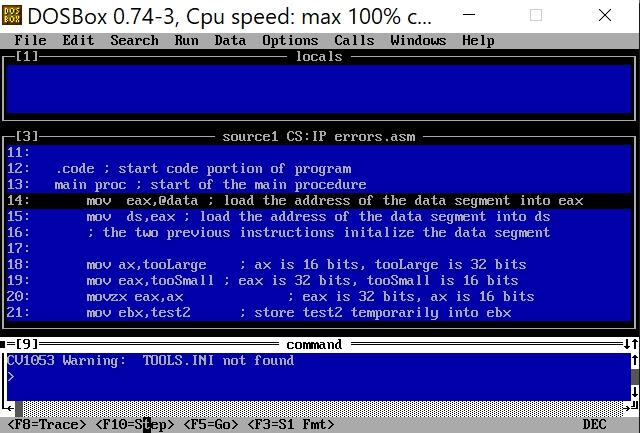
\includegraphics[width=\linewidth]{images/firstCV.jpg}
  \caption{Initial CodeView Screen.}
  \label{fig:cv1}
\end{figure}
A screen like this one (Figure \ref{fig:cv1}) will pop up. 
The next thing we will do is open the Register window (click {\code Windows -> Register}).  Since we have one memory location changing we'll add a Watch (click {\code Data->Add Watch} and type in test1 and hit ok).  
\begin{figure}
  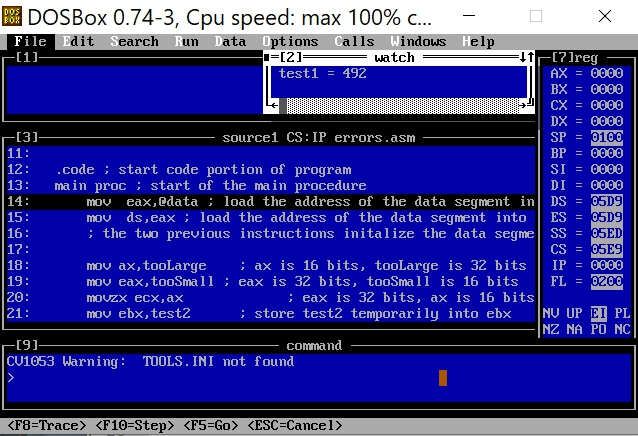
\includegraphics[width=\linewidth]{images/watchCV.jpg}
  \caption{CodeView with Registers and a Watch.}
  \label{fig:cv2}
\end{figure}
The window now should look like this (Figure \ref{fig:cv2}). 

Now we can step through our code and see how the registers change, hit F10 to step through each line.  When the program is through, it has the final values of the registers, a garbage value for test1 since the program is over, and gives a peek at the assembled code (Figure \ref{fig:cv3}).  
\begin{figure}
  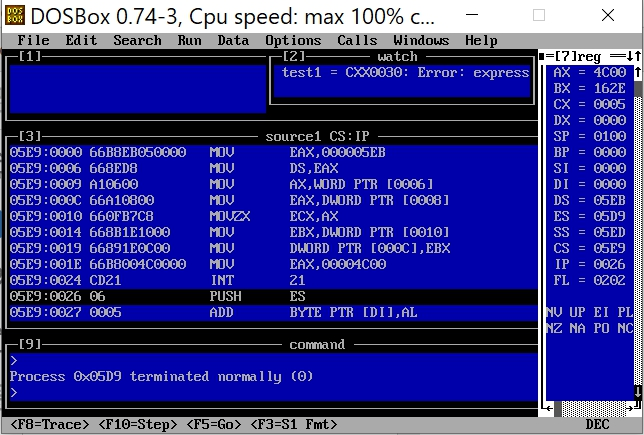
\includegraphics[width=\linewidth]{images/endCV.jpg}
  \caption{CodeView after program runs.}
  \label{fig:cv3}
\end{figure}
Just like in most IDEs you are used to you can also set break points instead of running every line and once you have procedures you can use F8 to trace the procedure or F10 to step over it.  
% do fib for lecture and debug it on the fly do errors for this to show registers and memory
%
\subsection{DOSBox/MASM Quirks}
\begin{itemize}
\item Sometimes your mouse will get stuck in the DOSBox window if you hit alt-Tab that will switch to another open window on your computer and will free your mouse. 
\item If you have an infinite loop or otherwise want to force your program to close, the best way is to just close DOSBox altogether and restart. 
\item In CodeView sometimes it will stop recognizing the mouse, but the keyboard will still work so you can use the shortcut keys.  If you need to choose something from the Menu you can type Alt-F to open the File Menu then you can use the arrow keys and then enter to select what you need.  To exit you can simply type Alt-F4.    
%more?
\end{itemize} %masm
%-*- latex -*-
\chapter{Subprograms}

This chapter looks at using subprograms to make modular programs and to
interface with high level languages (like C). Functions and procedures are
high level language examples of subprograms.

The code that calls a subprogram and the subprogram itself must agree
on how data will be passed between them. These rules on how data will
be passed are called \emph{calling conventions}. \index{calling
convention} A large part of this chapter will deal with the standard C
calling conventions that can be used to interface assembly subprograms
with C programs. This (and other conventions) often pass the addresses
of data (\emph{i.e.} pointers) to allow the subprogram to access the
data in memory.

\section{Indirect Addressing\index{indirect addressing|(}}

Indirect addressing allows registers to act like pointer variables. To
indicate that a register is to be used indirectly as a pointer, it is
enclosed in square brackets ({\code []}). For example:
%tested in subproc0.asm
\begin{lstlisting}[language={[x86masm]Assembler}]
      mov    ax, data     ; normal direct memory addressing of a word
      mov    ebx, offset data      ; ebx = & data
      mov    ax, [ebx]      ; ax = *ebx
\end{lstlisting}
\MarginNote{Note: Lines 1 and 3 perform the same operation.}
Because AX holds a word, line~3 reads a word starting at the address stored 
in EBX.  What EBX is assumed to point to is completely determined by what
instructions are used. Furthermore, even the fact that EBX is a pointer is
completely determined by the what instructions are used. If EBX is used
incorrectly, often there will be no assembler error; however, the program
will not work correctly. This is one of the many reasons that assembly
programming is more error prone than high level programming.

All the 32-bit general purpose (EAX, EBX, ECX, EDX) and index (ESI, EDI)
registers can be used for indirect addressing. 
\index{indirect addressing|)}

\section{Simple Subprogram Example\index{subprogram|(}}

A subprogram is an independent unit of code that can be used from different
parts of a program. In other words, a subprogram is like a function in C. A
jump can be used to invoke the subprogram, but returning presents a problem.
If the subprogram is to be used by different parts of the program, it must
return back to the section of code that invoked it. Thus, the jump back from
the subprogram can not be hard coded to a label. The code below shows how this
could be done using the indirect form of the {\code JMP} instruction. This 
form of the instruction uses the value of a register to determine where to
jump to (thus, the register acts much like a \emph{function pointer} in C.)
Here is a program that uses a subprogram to get a digit from the user.
\lstinputlisting{../code/ch5/subproc1.asm}

The {\code get\_digit} subprogram uses a simple, register-based calling
convention. It expects the EBX register to hold the address of the
BYTE to store the digit input into and the ECX register to hold the
code address of the instruction to jump back to. In line~22,
the {\code ret1} label is used to compute this return address. The {\code \$} 
operator could have been used to compute the return
address. The {\code \$} operator returns the current address for the
line it appears on. The expression {\code \$ + 8} computes the address
of the {\code ret1} label on line~24.

Both of these return address computations are awkward. The first method
requires a label to be defined for each subprogram call. The second method
does not require a label, but does require careful thought. If a near jump
was used instead of a short jump, the number to add to {\code \$} would not
be 8! Fortunately, there is a much simpler way to invoke subprograms. This
method uses the \emph{stack}.

\section{The Stack\index{stack|(}}

Many CPUs have built-in support for a stack. A stack is a Last-In First-Out
(\emph{LIFO}) list. The stack is an area of memory that is organized in this
fashion. The {\code PUSH} instruction adds data to the stack and the
{\code POP} instruction removes data. The data removed is always the last
data added (that is why it is called a last-in first-out list).

The SS segment register specifies the segment that contains the stack (usually
this is the same segment data is stored into). The ESP register contains the
address of the data that would be removed from the stack. This data is said
to be at the \emph{top} of the stack. Data can only be added in double word
units. That is, one can not push a single byte on the stack.

The {\code PUSH} instruction inserts a double word\footnote{Actually
words can be pushed too, but in 32-bit protected mode, it is easier to
work with only double words on the stack.} on the stack by subtracting
4 from ESP and then stores the double word at {\code [ESP]}. The
{\code POP} instruction reads the double word at {\code [ESP]} and
then adds 4 to ESP. The code below demonstrates how these instructions
work and assumes that ESP is initially {\code 0100H}.
%tested in stack.asm
\begin{lstlisting}[language={[x86masm]Assembler}]
    push   dword ptr 1   ; 1 stored at 00FCh, ESP = 00FCh
    push   dword ptr 2   ; 2 stored at 00F8h, ESP = 00F8h
    push   dword ptr 3   ; 3 stored at 00F4h, ESP = 00F4h
    pop    eax        ; EAX = 3, ESP = 00F8h
    pop    ebx        ; EBX = 2, ESP = 00FCh
    pop    ecx        ; ECX = 1, ESP = 0100h
\end{lstlisting}

The stack can be used as a convenient place to store data temporarily. It is
also used for making subprogram calls, passing parameters and local
variables.

The 80x86 also provides a {\code PUSHA} instruction (push all) that pushes the values
of EAX, EBX, ECX, EDX, ESI, EDI and EBP registers (not in this order). The
{\code POPA} instruction (pop all) can be used to pop them all back off.
\index{stack|)}

\section{The CALL and RET Instructions\index{subprogram!calling|(}}
\index{CALL|(}
\index{RET|(}
The 80x86 provides two instructions that use the stack to make calling
subprograms quick and easy. The CALL instruction makes an
unconditional jump to a subprogram and \emph{pushes} the address of
the next instruction on the stack. The RET instruction
\emph{pops off} an address and jumps to that address. When using these
instructions, it is very important that one manage the stack correctly
so that the right number is popped off by the RET instruction!

The previous program can be rewritten to use these new instructions by 
changing lines~21 to 24 to be:
%tested in subproc2.asm
\begin{lstlisting}[language={[x86masm]Assembler}, firstnumber=21]
      mov    ebx, offset input
      ; don't need this anymore
      call   get_digit
      ; this either
\end{lstlisting}
and change the subprogram {\code get\_digit} to:
\begin{lstlisting}[language={[x86masm]Assembler}]
get_digit:
    mov ah, 1
    int 21h
    and al, 0fh     ; char to int
    mov [ebx], al   ; store input into memory
    ret         ; jump back to caller
\end{lstlisting}

There are several advantages to CALL and RET:
\begin{itemize}
\item It is simpler!
\item It allows subprograms calls to be nested easily. Notice that
{\code get\_digit} could call {\code read\_char}. This call pushes another address
on the stack. At the end of {\code read\_char}'s code is a RET that pops
off the return address and jumps back to {\code get\_digit}'s code. Then when
{\code get\_digit}'s RET is executed, it pops off the return address that 
jumps back to {\code main}. This works correctly because of the LIFO
property of the stack.
%tested in subproc2.asm
\begin{lstlisting}[language={[x86masm]Assembler}]
get_digit:
    call read_char
    and al, 0fh     ; char to int
    mov [ebx], al   ; store input into memory
    ret         ; jump back to caller

read_char:
    mov ah, 1
    int 21h
    ret
\end{lstlisting}
\end{itemize}

Remember it is \emph{very} important to pop off all data that is pushed
on the stack. For example, consider the following:
%tested in subproc2.asm
\begin{lstlisting}[language={[x86masm]Assembler}]
get_digit:
    mov ah, 1
    int 21h
    and al, 0fh     ; char to int
    mov [ebx], al   ; store input into memory
    push eax
    ret         ; pops off eax value, not the return address!! 
\end{lstlisting}
This code would not return correctly!
\index{RET|)}
\index{CALL|)}

\section{Calling Conventions\index{calling convention|(}}

When a subprogram is invoked, the calling code and the subprogram (the
\emph{callee}) must agree on how to pass data between them. High-level
languages have standard ways to pass data known as \emph{calling 
conventions}. For high-level code to interface with assembly language, the
assembly language code must use the same conventions as the high-level
language. The calling conventions can differ from compiler to compiler or
may vary depending on how the code is compiled (\emph{e.g.} if
optimizations are on or not). One universal convention is that the code will
be invoked with a {\code CALL} instruction and return via a {\code RET}.

Calling conventions
allow one to create subprograms that are \emph{reentrant}. A reentrant
subprogram may be called at any point of a program safely (even inside
the subprogram itself).

\subsection{"Passing" parameters using registers}
As we saw above, the easiest way you can "pass" parameters is to use the registers.  
I say pass in quotes because you aren't doing anything extra like you do in C++.  Nevertheless,
you can use the existing values in your subprogram.  The changes
 you make will change the registers back in main, similar to passing by reference. 
 \subsubsection{Passing registers by value}
 Sometimes you might want to change the registers in the procedure, but not have those changes
 reflected in main.  This is similar to a local variable in C++ or passing a parameter by value.  There are two 
 common ways to do this, the first is to use push and pop to keep the registers from changing, 
 here is an example from earlier, but now the value of eax is preserved:
 %tested in subproc3.asm
 \begin{lstlisting}[language={[x86masm]Assembler}]
 get_digit:
    push eax
    mov ah, 1
    int 21h
    and al, 0fh     ; char to int
    mov [ebx], al   ; store input into memory
    pop eax
    ret        
\end{lstlisting}
The second way does the exact same thing, but without push and pop cluttering your code 
(the assembler adds those later).  To preserve the registers this way you use PROC with USES, 
this looks cleaner, and is explicit that EAX is being preserved.  
%tested in subproc3.asm
 \begin{lstlisting}[language={[x86masm]Assembler}]
get_digit proc uses eax
    mov ah, 1
    int 21h
    and al, 0fh     ; char to int
    mov [ebx], al   ; store input into memory
    ret         
get_digit endp
\end{lstlisting}
Note the ENDP at the bottom, this is needed to close the procedure.  We didn't need to do this when
we were using a named location for our procedure, but it becomes necessary when you use PROC.
Since we use this we also have to move {\code MAIN ENDP} above the procedure because we can't 
have nested procedures. 
\subsection{Passing parameters on the stack\index{stack|(}\index{stack!parameters|(}}

Parameters to a subprogram may be passed on the stack. They are pushed onto
the stack before the {\code CALL} instruction. Just as in C, if the
parameter is to be changed by the subprogram, the \emph{address} of the 
data must be passed, not the \emph{value}. If the parameter's size is less
than a double word, it must be converted to a double word before being pushed.

The parameters on the stack are not popped off by the subprogram, instead
they are accessed from the stack itself. Why?
\begin{itemize}
\item Since they have to be pushed on the stack before the {\code CALL}
instruction, the return address would have to be popped off first (and
then pushed back on again).
\item Often the parameters will have to be used in several places in the
subprogram. Usually, they can not be kept in a register for the entire
subprogram and would have to be stored in memory. Leaving them on the
stack keeps a copy of the data in memory that can be accessed at any
point of the subprogram.
\end{itemize}

\begin{figure}
\centering
\begin{tabular}{l|c|}
\cline{2-2}
&  \\ \cline{2-2}
ESP + 4 & Parameter \\ \cline{2-2}
ESP     & Return address \\ \cline{2-2}
 & \\ \cline{2-2}
\end{tabular}
\caption{}
\label{fig:stack1}
\end{figure}
Consider 
%\MarginNote{When using indirect addressing, the 80x86 processor 
%accesses different segments depending on what registers are used in the
%indirect addressing expression. ESP (and EBP) use the stack segment while
%EAX, EBX, ECX and EDX use the data seg\-ment. However, this is usually 
%unimportant for most protected mode programs, because for them the data 
%and stack segments are the same.}
a subprogram that is passed a single parameter on the stack. When
the subprogram is invoked, the stack looks like Figure~\ref{fig:stack1}.
The parameter can be accessed using indirect addressing ({\code [ESP+4]}
\footnote{It is legal to add a constant to a register when using indirect
addressing. More complicated expressions are possible too. This topic is covered
in the next chapter}).
\begin{figure}
\centering
\begin{tabular}{l|c|}
\cline{2-2}
&  \\ \cline{2-2}
ESP + 8 & Parameter \\ \cline{2-2}
ESP + 4 & Return address \\ \cline{2-2}
ESP     & subprogram data \\ \cline{2-2}
\end{tabular}
\caption{}
\label{fig:stack2}
\end{figure}

\begin{figure}[t]
 \begin{lstlisting}[language={[x86masm]Assembler}]
subprogram_label:
      push   ebp           ; save original EBP value on stack
      mov    ebp, esp      ; new EBP = ESP
; subprogram code
      pop    ebp           ; restore original EBP value
      ret
\end{lstlisting}
\caption{General subprogram form \label{fig:subskel1}}
\end{figure}

If the stack is also used inside the subprogram to store data, the
number needed to be added to ESP will change. For example,
Figure~\ref{fig:stack2} shows what the stack looks like if a DWORD is
pushed the stack. Now the parameter is at {\code ESP + 8} not {\code
ESP + 4}. Thus, it can be very error prone to use ESP when referencing
parameters. To solve this problem, the 80386 supplies another register
to use: EBP. This register's only purpose is to reference data on the
stack. The C calling convention mandates that a subprogram first save
the value of EBP on the stack and then set EBP to be equal to ESP.
This allows ESP to change as data is pushed or popped off the stack
without modifying EBP. At the end of the subprogram, the original
value of EBP must be restored (this is why it is saved at the start of
the subprogram.)  Figure~\ref{fig:subskel1} shows the general form of
a subprogram that follows these conventions.

\begin{figure}[t]
\centering
\begin{tabular}{ll|c|}
\cline{3-3}
&  & \\ \cline{3-3}
ESP + 8 & EBP + 8 & Parameter \\ \cline{3-3}
ESP + 4 & EBP + 4 & Return address \\ \cline{3-3}
ESP     & EBP     & saved EBP \\ \cline{3-3}
\end{tabular}
\caption{}
\label{fig:stack3}
\end{figure}


Lines 2 and 3 in Figure~\ref{fig:subskel1} make up the general \emph{prologue}
of a subprogram. Lines 5 and 6 make up the \emph{epilogue}. 
Figure~\ref{fig:stack3} shows what the stack looks like immediately
after the prologue. Now the parameter can be access with {\code [EBP + 8]}
at any place in the subprogram without worrying about what else has
been pushed onto the stack by the subprogram.

After the subprogram is over, the parameters that were pushed on the
stack must be removed. The C calling convention \index{calling
convention!C} specifies that the caller code must do this. Other
conventions are different. For example, the Pascal calling convention
\index{calling convention!Pascal} specifies that the subprogram must
remove the parameters.  (There is another form of the RET \index{RET}
instruction that makes this easy to do.) Some C compilers support this
convention too. 

\begin{figure}[t]
 \begin{lstlisting}[language={[x86masm]Assembler}]
      push   dword ptr 1        ; pass 1 as parameter
      call   funC
      add    esp, 4         ; remove parameter from stack
\end{lstlisting}
\caption{Sample C style subprogram call \label{fig:subcallC}}
\end{figure}

\begin{figure}[t]
 \begin{lstlisting}[language={[x86masm]Assembler}]
      push   dword ptr 1        ; pass 1 as parameter
      call   funPascal
      ...
      funPascal PROC
          ;subprogram code
          ret 4 ;remove parameter from stack
       funPascal ENDP
\end{lstlisting}
\caption{Sample Pascal style subprogram call \label{fig:subcallP}}
\end{figure}

Figure~\ref{fig:subcallC} shows how a subprogram using the C calling
convention would be called. Line~3 removes the parameter from the
stack by directly manipulating the stack pointer. A {\code POP}
instruction could be used to do this also, but would require the
useless result to be stored in a register. Actually, for this
particular case, many compilers would use a {\code POP ECX}
instruction to remove the parameter. The compiler would use a {\code
POP} instead of an {\code ADD} because the {\code ADD} requires more
bytes for the instruction. However, the {\code POP} also changes ECX's
value!  Figure~\ref{fig:subcallP} show how a subprogram using the Pascal
calling convention would remove the parameter from the stack. \\

Next is another example program with two subprograms that use
the C calling conventions discussed above. Line~64 (and other lines)
shows that multiple data and code segments may be declared in a single
source file. They will be combined into single data and code segments
in the linking process. Splitting up the data and code into separate
segments allow the data that a subprogram uses to be defined close by
the code of the subprogram.
\index{stack!parameters|)}

\lstinputlisting{../code/ch5/numSum.asm} %numSum


\subsection{Local variables on the stack\index{stack!local variables|(}}

The stack can be used as a convenient location for local variables. This is
exactly where C stores normal (or \emph{automatic} in C lingo) variables.
Using the stack for variables is important if one wishes subprograms to be
reentrant. A reentrant subprogram will work if it is invoked at any place,
including the subprogram itself. In other words, reentrant subprograms
can be invoked \emph{recursively}. Using the stack for variables also saves
memory. Data not stored on the stack is using memory from the beginning of
the program until the end of the program (C calls these types of variables
\emph{global} or \emph{static}). Data stored on the stack only use memory
when the subprogram they are defined for is active.

\begin{figure}[t]
 \begin{lstlisting}[language={[x86masm]Assembler}]
subprogram_label:
      push   ebp                ; save original EBP value on stack
      mov    ebp, esp           ; new EBP = ESP
      sub    esp, LOCAL_BYTES   ; = # bytes needed by locals
; subprogram code
      mov    esp, ebp           ; deallocate locals
      pop    ebp                ; restore original EBP value
      ret
\end{lstlisting}
\caption{General subprogram form with local variables\label{fig:subskel2}}
\end{figure}

\begin{figure}[t]
\begin{lstlisting}[language=C++,frame=tlrb]{}
void calc_sum( int n, int *sumP) {
  int i, sum = 0;

  for( i=1; i <= n; i++ ) {
    sum += i;
   }
  *sumP = sum;
}
\end{lstlisting}
\caption{C version of sum \label{fig:Csum}}
\end{figure}

%this is in subproc4.asm
\begin{figure}[t]
 \begin{lstlisting}[language={[x86masm]Assembler}]
; stack has the address of sumP and the value of n
cal_sum:
      push   ebp
      mov    ebp, esp
      sub    esp, 4               ; make room for local sum
      
      mov    dword ptr [ebp - 4], 0   ; sum = 0
      mov    ebx, 1               ; ebx (i) = 1
for_loop:
      cmp    ebx, [ebp+8]         ; is i <= n?
      jnle   end_for

      add    [ebp-4], ebx         ; sum += i
      inc    ebx
      jmp    short for_loop

end_for:
      mov    ebx, [ebp+12]        ; ebx = sumP
      mov    eax, [ebp-4]         ; eax = sum
      mov    [ebx], eax           ; *sumP = sum;

      mov    esp, ebp
      pop    ebp
      ret
 \end{lstlisting}
\caption{Assembly version of sum\label{fig:Asmsum}}
\end{figure}

Local variables are stored right after the saved EBP value in the stack.
They are allocated by subtracting the number of bytes required from ESP
in the prologue of the subprogram. Figure~\ref{fig:subskel2} shows the 
new subprogram skeleton. The EBP register is used to access local variables.
Consider the C function in Figure~\ref{fig:Csum}. Figure~\ref{fig:Asmsum}
shows how the equivalent subprogram could be written in assembly.

\begin{figure}[t]
\centering
\begin{tabular}{ll|c|}
\cline{3-3}
ESP + 16 & EBP + 12 & address of {\code sumP} \\ \cline{3-3}
ESP + 12 & EBP + 8  & {\code n} \\ \cline{3-3}
ESP + 8  & EBP + 4  & Return address \\ \cline{3-3}
ESP + 4  & EBP      & saved EBP \\ \cline{3-3}
ESP      & EBP - 4  & {\code sum} \\ \cline{3-3}
\end{tabular}
\caption{}
\label{fig:SumStack}
\end{figure}

Figure~\ref{fig:SumStack} shows what the stack looks like after the
prologue of the program in Figure~\ref{fig:Asmsum}. This section of
the stack that contains the parameters, return information and local
variable storage is called a \emph{stack frame}. Every invocation of
a C function creates a new stack frame on the stack.

\begin{figure}[t]
 \begin{lstlisting}[language={[x86masm]Assembler}]
subprogram_label:
      enter  LOCAL_BYTES, 0     ; = # bytes needed by locals
; subprogram code
      leave
      ret
 \end{lstlisting}
\caption{General subprogram form with local variables using 
{\code ENTER} and {\code LEAVE}\label{fig:subskel3}}
\end{figure}

%\MarginNote{Despite the fact that {\code ENTER} and {\code LEAVE} simplify
%the prologue and epilogue they are not used very often. Why? Because
%they are slower than the equivalent simpler instructions! This is an
%example of when one can not assume that a one instruction sequence is
%faster than a multiple instruction one.} 
The prologue and epilogue of a subprogram can be simplified by using
two special instructions that are designed specifically for this
purpose. The {\code ENTER} instruction performs the prologue code and the
{\code LEAVE} performs the epilogue. The {\code ENTER} instruction
takes two immediate operands. For the C calling convention, the second
operand is always 0. The first operand is the number of bytes needed by
local variables. The {\code LEAVE} instruction has no
operands. Figure~\ref{fig:factorial} shows how these instructions are
used. 

\index{stack!local variables|)}
\index{stack|)}
\index{calling convention|)}
\index{subprogram!calling|)}
\section{Multi-Module Programs\index{multi-module programs|(}}

A \emph{multi-module program} is one composed of more than one object
file.  The numSum.asm example program above is a multi-module
program. It consists of the Assembly driver object file and the assembly
object file. Recall that the linker
combines the object files into a single executable program. The linker
must match up references made to each label in one module (\emph{i.e.}
object file) to its definition in another module. In order for module
A to use a label defined in module B, the {\code extern} directive
must be used. After the {\code extern} \index{directive!extern}
directive comes a label and then {\code :proc} to let it know the label is a procedure. 
The directive tells the assembler to treat these labels as \emph{external} to the
module. That is, these are labels that can be used in this module, but
are defined in another. The {\code printInc.lib} file defines the
{\code printDec}, \emph{etc.} routines as external.

\index{multi-module programs|)}

\section{Reentrant and Recursive Subprograms\index{recursion|(}}

\index{subprogram!reentrant|(}
A reentrant subprogram must satisfy the following properties:
\begin{itemize}
\item It must not modify any code instructions. In a high level language
this would be difficult, but in assembly it is not hard for a program to
try to modify its own code. For example:
%this is tested in subproc5.asm
 \begin{lstlisting}[language={[x86masm]Assembler},numbers=none]
  mov word ptr [cs:$+9], 5    ; copy 5 into the word 7 bytes ahead
  add ax, 2               ; previous statement changes 2 to 5!
\end{lstlisting}
This code would work in real mode, but in protected mode operating systems 
the code segment is marked as read only. When the first line above executes,
the program will be aborted on these systems. This type of programming is
bad for many reasons. It is confusing, hard to maintain and does not allow
code sharing (see below).

\item It must not modify global data (such as data in the {\code data} and
the {\code bss} segments). All variables are stored on the stack.

\end{itemize}

There are several advantages to writing reentrant code.
\begin{itemize}
\item A reentrant subprogram can be called recursively.
\item A reentrant program can be shared by multiple processes. On many
multi-tasking operating systems, if there are multiple instances of a
program running, only \emph{one} copy of the code is in memory. Shared
libraries and DLL's (\emph{Dynamic Link Libraries}) use this idea as well.
\item Reentrant subprograms work much better in \emph{multi-threaded}
\footnote{A multi-threaded program has multiple threads of execution. That
is, the program itself is multi-tasked.} pro\-grams. Windows 9x/NT and most
UNIX-like operating systems (Solaris, Linux, \emph{etc.}) support 
multi-threaded programs.
\end{itemize}
\index{subprogram!reentrant|)}

\subsection{Recursive subprograms}

These types of subprograms call themselves. The recursion can be either
\emph{direct} or \emph{indirect}. Direct recursion occurs when a subprogram,
say {\code foo}, calls itself inside {\code foo}'s body. Indirect recursion
occurs when a subprogram is not called by itself directly, but by another
subprogram it calls. For example, subprogram {\code foo} could call
{\code bar} and {\code bar} could call {\code foo}.

Recursive subprograms must have a \emph{termination condition}. When
this condition is true, no more recursive calls are made. If a
recursive routine does not have a termination condition or the condition
never becomes true, the recursion will never end (much like an infinite
loop).

%also in subproc5.asm
\begin{figure}
 \begin{lstlisting}[language={[x86masm]Assembler}]
; finds n!
factorial proc
    enter 0,0 ; sets up stack frame
    mov    eax, [ebp+4] ; eax = n retrieve parameter from stack
    cmp    eax, 1 ; check termination condition
    jbe    term_cond    ; if n <= 1, terminate
    dec    eax    ; n--
    push   eax    ; call with (n-1)
    call   factorial ; eax = fact(n-1)
    mul    dword ptr [ebp+4]   ; edx:eax = eax * [ebp+4]
    term_cond:
    leave ; terminates stack frame
    ret 1 ; clean up the eax we pushed earlier
factorial endp
\end{lstlisting}
\caption{Recursive factorial function\label{fig:factorial}}
\end{figure}

\begin{figure}
\centering
%\includegraphics{factStack.eps}
\input{factStack.latex}
\caption{Stack frames for factorial function\label{fig:factStack}}
\end{figure}

Figure~\ref{fig:factorial} shows a function that calculates factorials
recursively. It could be called from C with:
\begin{lstlisting}[stepnumber=0]{}
x = factorial(3);         /* find 3! */
\end{lstlisting}
Figure~\ref{fig:factStack} shows what the stack looks like at its deepest
point for the above function call.


%Figures~\ref{fig:rec2C} and \ref{fig:rec2Asm} show another more
%complicated recursive example in C and assembly, respectively. What is
%the output is for {\code factorial(3)}? Note that the {\code ENTER} instruction
%creates a new {\code i} on the stack for each recursive call. Thus, each
%recursive instance of {\code f} has its own independent variable {\code i}.
%Defining {\code i} as a double word in the {\code data} segment would not
%work the same. 
\index{recursion|)}

\index{subprogram|)}
 %procs 
% -*-latex-*-
\chapter{Arrays}
\index{arrays|(}
\section{Introduction}

An \emph{array} is a contiguous block of data in memory. Each element
of the list must be the same type and use exactly the same number of bytes
of memory for storage. Because of these properties, arrays allow efficient
access of the data by its position (or index) in the array. The address
of any element can be computed by knowing three facts:
\begin{itemize}
\item The address of the first element of the array.
\item The number of bytes in each element
\item The index of the element
\end{itemize}

It is convenient to consider the index of the first element of the array
to be zero (just as in C). It is possible to use other values for the
first index, but it complicates the computations.

\subsection{Defining arrays\index{arrays!defining|(}}

\begin{figure}[t]
%tested in array1.asm
\begin{lstlisting}[language={[x86masm]Assembler}]
.data
	; define array of 10 double words initialized to 1,2,..,10
	a1 dd 1, 2, 3, 4, 5, 6, 7, 8, 9, 10
	; define array of 10 words initialized to 0
	a2 dw  0, 0, 0, 0, 0, 0, 0, 0, 0, 0
	; same as before using dup
	a3 dw 10 dup (0)
	; define array of bytes with 200 0's and then 100 1's
	a4 db 200 dup (0)
	   db 100 dup (1)
	; define an array of 10 uninitialized double words
	a5 dd 10 dup (?)
	; define an array of 100 uninitialized words
	a6 dw 100 dup (?)
\end{lstlisting}
\caption{Defining arrays\label{fig:DataArrays}}
\end{figure}

\subsubsection{Defining arrays in the {\code data} segment
               \index{arrays!defining!static}}

To define an initialized array in the {\code data} segment, use the
normal {\code db}, {\code dw}, \emph{etc.} 
\index{directive!D\emph{X}}directives. MASM also provides a useful directive
named {\code DUP} \index{directive!DUP} that can be used to repeat a statement many times
without having to duplicate the statements by hand.
Figure~\ref{fig:DataArrays} shows several examples of these.

To define an uninitialized array, use the
{\code ?} \index{directive!?}
directive. Figure~\ref{fig:DataArrays} also shows examples of these
types of definitions.

\begin{figure}[t]
\centering
\begin{tabular}{l|c|ll|c|}
\cline{2-2} \cline{5-5}
EBP - 1  & char    & \hspace{2em} &           & \\
\cline{2-2}
         & unused  &              &           & \\
\cline{2-2}
EBP - 8  & dword 1 &              &           & \\
\cline{2-2}
EBP - 12 & dword 2 &              &           & word \\
\cline{2-2}
         &         &              &           & array \\
         &         &              &           & \\
         & word    &              &           & \\
         & array   &              & EBP - 100 & \\
\cline{5-5}
         &         &              & EBP - 104 & dword 1 \\
\cline{5-5}
         &         &              & EBP - 108 & dword 2 \\
\cline{5-5}
         &         &              & EBP - 109 & char \\
\cline{5-5}
EBP - 112 &        &              &           & unused \\
\cline{2-2} \cline{5-5}
\end{tabular}
\caption{Arrangements of the stack\label{fig:StackLayouts}}
\end{figure}

\subsubsection{Defining arrays as local variables on the stack\index{arrays!defining!local variable}}

There is no direct way to define a local array variable on the
stack. As before, one computes the total bytes required by \emph{all}
local variables, including arrays, and subtracts this from ESP (either
directly or using the {\code ENTER} instruction). For example, if a
function needed a character variable, two double word integers and a
50 element word array, one would need $1 + 2 \times 4 + 50 \times 2 =
109$ bytes. However, the number subtracted from ESP should be a
multiple of four (112 in this case) to keep ESP on a double word
boundary. One could arrange the variables inside this 109 bytes in
several ways. Figure~\ref{fig:StackLayouts} shows two possible ways. The
unused part of the first ordering is there to keep the double words on
double word boundaries to speed up memory accesses.
\index{arrays!defining|)}

\subsection{Accessing elements of arrays\index{arrays!accessing|(}}

The {\code [ ]} operator in assembly language is much more versatile than C.  You can
use it similarly to how you might use it in C to access an array, but to
access the correct element of an array, its address must be computed. Consider
the following two array definitions:
%tested in array2.asm
\begin{lstlisting}[language={[x86masm]Assembler}]
array1  db 5, 4, 3, 2, 1     ; array of bytes
array2  dw 5, 4, 3, 2, 1     ; array of words
array3  dd 5, 4, 3, 2, 1     ; array of double words
\end{lstlisting}
Here are some examples using these arrays:
\begin{lstlisting}[language={[x86masm]Assembler}]
	mov    al, [array1]             ; al = array1[0]
	mov    al, array1[1]         ; al = array1[1]
	mov    [array1 + 3], al         ; array1[3] = al
	mov    ax, array2             ; ax = array2[0]
	mov    ax, array2[2]         ; ax = array2[1] (NOT array2[2]!)
	mov    [array2 + 6], ax         ; array2[3] = ax
	mov    ax, [array2 + 1]         ; ax = ??
\end{lstlisting}
In line~5, element 1 of the word array is referenced, not element 2. Why?
Words are two byte units, so to move to the next element of a word array,
one must move two bytes ahead, not one. Line~7 will read one byte from the
first element and one from the second. In C, the compiler looks at the type
of a pointer in determining how many bytes to move in an expression that
uses pointer arithmetic so that the programmer does not have to. However,
in assembly, it is up to the programmer to take the size of array elements
in account when moving from element to element. \index{ArrayOps(}Luckily, there is a way 
to calculate the important values associated with an array, see Table~\ref{tab:ArrayOps}.

\begin{table}[]
\begin{tabular}{ll}
\textbf{Command} & \textbf{Purpose}                    \\
type             & The number of bytes in each element \\
lengthof           & The number of elements in an array  \\
sizeof         & The number of bytes in an array    
\end{tabular}
\caption{Helpful Array Operators\label{tab:ArrayOps}}
\end{table}
\index{ArrayOps)}
%tested in array3.asm way 1
\begin{figure}[t]
\begin{lstlisting}[language={[x86masm]Assembler},frame=single]
	mov    ebx, offset array1           ; ebx = address of array1
	mov    dx, 0                 ; dx will hold sum
	mov    ah, 0                 ; ?
	mov    ecx, 5
lp:
	mov    al, [ebx]             ; al = *ebx
	add    dx, ax                ; dx += ax (not al!)
	inc    ebx                   ; bx++
	loop   lp
\end{lstlisting}
\caption{Summing elements of an array (Version 1)\label{fig:SumArray1}}
\end{figure}
%tested in array3.asm way 2
\begin{figure}[t]
\begin{lstlisting}[language={[x86masm]Assembler},frame=single]
      mov    ebx, offset array1           ; ebx = address of array1
      mov    dx, 0                 ; dx will hold sum
      mov    ecx, 5
lp:
      add    dl, [ebx]             ; dl += *ebx
      jnc    next                  ; if no carry goto next
      inc    dh                    ; inc dh
next:
      inc    ebx                   ; bx++
      loop   lp
\end{lstlisting}
\caption{Summing elements of an array (Version 2)\label{fig:SumArray2}}
\end{figure}
%tested in array3.asm way 3
\begin{figure}[t]
\begin{lstlisting}[language={[x86masm]Assembler},frame=single]
      mov    ebx, offset array1           ; ebx = address of array1
      mov    dx, 0                 ; dx will hold sum
      mov    ecx, 5
lp:
      add    dl, [ebx]             ; dl += *ebx
      adc    dh, 0                 ; dh += carry flag + 0
      inc    ebx                   ; bx++
      loop   lp
\end{lstlisting}
\caption{Summing elements of an array (Version 3)\label{fig:SumArray3}}
\end{figure}

Figure~\ref{fig:SumArray1} shows a code snippet that adds all the
elements of {\code array1} in the previous example code. In
line 7, AX is added to DX. Why not AL? First, the
two operands of the {\code ADD} instruction must be the same
size. Secondly, it would be easy to add up bytes and get a sum that
was too big to fit into a byte. By using DX, sums up to 65,535 are
allowed. However, it is important to realize that AH is being added
also.  This is why AH is set to zero\footnote{Setting AH to zero is
implicitly assuming that AL is an unsigned number. If it is signed,
the appropriate action would be to insert a {\code CBW} instruction
between lines~6 and 7} in line~3.

Figures~\ref{fig:SumArray2} and \ref{fig:SumArray3} show two alternative
ways to calculate the sum. The differences are mostly around lines~6 and 7
of each Figure.

\subsection{More advanced indirect addressing\index{indirect addressing!arrays|(}}

Not surprisingly, indirect addressing is often used with arrays. The most
general form of an indirect memory reference is:
\begin{center}
{\code [ \emph{base reg} + \emph{factor}*\emph{index reg} + 
      \emph{constant}]}
\end{center}
where:
\begin{description}
\item[base reg] is one of the registers EAX, EBX, ECX, EDX, EBP, ESP, ESI
                or EDI.
\item[factor] is either 1, 2, 4 or 8 . (If 1, factor is omitted.)
\item[index reg] is one of the registers EAX, EBX, ECX, EDX, EBP, ESI, EDI.
                 (Note that ESP is not in list.)
\item[constant] is a 32-bit constant. The constant can be a label (or
                a label expression).
\end{description}

%\subsection{Example}
Figure~\ref{fig:SumArray4} is another sum array example that uses the general form. 

%tested in array4.asm
\begin{figure}[t]
\begin{lstlisting}[language={[x86masm]Assembler},frame=single]
	mov    ebx, offset array3     ; ebx = address of array3
	mov    edx, 0                 ; edx will hold sum
	mov    ecx, 5                 ; ecx is our loop counter
lp:            ;[baseReg + factor*indexReg + constant]
	add    edx, [ebx+(type array3)*ecx-(type array3)]; edx += array3[ecx-1]
	loop   lp
\end{lstlisting}
\caption{Summing elements of an array (Version 4)\label{fig:SumArray4}}
\end{figure}

\index{indirect addressing!arrays|)}
\index{arrays!accessing|)}

\subsubsection{The {\code LEA} instruction\index{LEA|(}}

The {\code LEA} instruction is used to calculate addresses instead of 
{\code offset}. In addition to this, you could use it for other purposes. A fairly
common one is for fast computations. Consider the following:
%tested in array4.asm
\begin{lstlisting}[language={[x86masm]Assembler},numbers=none]
      lea    ebx, [4*eax + eax]
\end{lstlisting}
This effectively stores the value of $5 \times \mathtt{EAX}$ into EBX.
Using {\code LEA} to do this is both easier and faster than using
{\code MUL}\index{MUL}. However, one must realize that the expression
inside the square brackets \emph{must} be a legal indirect address.
Thus, for example, this instruction can not be used to multiple by 6
quickly.
\index{LEA|)}


\subsection{Multidimensional Arrays\index{arrays!multidimensional|(}}

Multidimensional arrays are not really very different than the plain
one dimensional arrays already discussed. In fact, they are represented 
in memory as just that, a plain one dimensional array.

\subsubsection{Two Dimensional Arrays\index{arrays!multidimensional!two dimensional|(}}
Not surprisingly, the simplest multidimensional array is a two dimensional
one. A two dimensional array is often displayed as a grid of elements. Each
element is identified by a pair of indices. By convention, the first index
is identified with the row of the element and the second index the column.

Consider an array with three rows and two columns defined as: 
\begin{lstlisting}[stepnumber=0]{}
  int a[3][2];
\end{lstlisting}
The C compiler would reserve room for a 6 ($= 2 \times 3$) integer array and
map the elements as follows:

\parbox{\textwidth}{
\vspace{0.5em}
\centering
\begin{tabular}{||l|c|c|c|c|c|c||}
\hline
Index & 0 & 1 & 2 & 3 & 4 & 5 \\
\hline
Element & a[0][0] & a[0][1] & a[1][0] & a[1][1] & a[2][0] & a[2][1]  \\
\hline
\end{tabular}
\vspace{0.5em}
}
\noindent What the table attempts to show is that the element referenced as 
{\code a[0][0]} is stored at the beginning of the 6 element one
dimensional array. Element {\code a[0][1]} is stored in the next
position (index~1) and so on. Each row of the two dimensional array is
stored contiguously in memory. The last element of a row is followed
by the first element of the next row. This is known as the
\emph{rowwise} representation of the array and is how a C/C++ compiler would
represent the array.

How does the compiler determine where {\code a[i][j]} appears in the rowwise
representation? A simple formula will compute the index from {\code i} and
{\code j}. The formula in this case is $2i + j$. It's not too hard to see how
this formula is derived. Each row is two elements long; so, the first element
of row $i$ is at position $2i$. Then the position of column $j$ is found by
adding $j$ to $2i$. This analysis also shows how the formula is generalized 
to an array with {\code N} columns: $N \times i + j$. Notice that the formula
does \emph{not} depend on the number of rows.

As an example, let us see how \emph{gcc} compiles the following code (using the
array {\code a} defined above):
\begin{lstlisting}[stepnumber=0]{}
  x = a[i][j];
\end{lstlisting}
The compiler essentially converts the code to:
\begin{lstlisting}[stepnumber=0]{}
  x = *(&a[0][0] + 2*i + j);
\end{lstlisting}
and in fact, the programmer could write this way with the same result.  The example code 
below shows how you might find the sum of a 2D array in assembly.

\lstinputlisting{../code/ch6/2dsum.asm}

There is nothing magical about the choice of the rowwise representation of the
array. A columnwise representation would work just as well: 

\parbox{\textwidth}{
\vspace{0.5em}
\centering
\begin{tabular}{||l|c|c|c|c|c|c||}
\hline
Index & 0 & 1 & 2 & 3 & 4 & 5 \\
\hline
Element & a[0][0] & a[1][0] & a[2][0] & a[0][1] & a[1][1] & a[2][1]  \\
\hline
\end{tabular}
\vspace{0.5em}
}
\noindent In the columnwise representation, each column is stored contiguously. 
Element {\code [i][j]} is stored at position $i + 3j$. Other languages
(FORTRAN, for example) use the columnwise representation. This is
important when interfacing code with multiple languages.
\index{arrays!multidimensional!two dimensional|)}

\subsubsection{Dimensions Above Two}
For dimensions above two, the same basic idea is applied. Consider a three
dimensional array:
\begin{lstlisting}[stepnumber=0]{}
  int b[4][3][2];
\end{lstlisting}
This array would be stored like it was four two dimensional arrays each of size
{\code [3][2]} consecutively in memory. The table below shows how it starts out:

\parbox{\textwidth}{
\vspace{0.5em}
\centering
\begin{tabular}{||l|c|c|c|c|c|c||}
\hline
Index & 0 & 1 & 2 & 3 & 4 & 5  \\
\hline
Element & b[0][0][0] & b[0][0][1]  & b[0][1][0] & b[0][1][1] & b[0][2][0]
&  b[0][2][1]  \\
\hline
\hline
Index & 6 & 7 & 8 & 9 & 10 & 11 \\
\hline
Element & b[1][0][0] & b[1][0][1] & b[1][1][0] & b[1][1][1]  & b[1][2][0] 
& b[1][2][1] \\
\hline
\end{tabular}
\vspace{0.5em}
}
\noindent The formula for computing the position of {\code b[i][j][k]}
is $6i + 2j + k$. The 6 is determined by the size of the {\code
[3][2]} arrays. In general, for an array dimensioned as {\code
a[L][M][N]} the position of element {\code a[i][j][k]} will be $M\times N\times i 
+ N \times j + k$. Notice again that the first
dimension ({\code L}) does not appear in the formula.

For higher dimensions, the same process is generalized. For an $n$ dimensional
array of dimensions $D_1$ to $D_n$, the position of element denoted by the
indices $i_1$ to $i_n$ is given by the formula:
\begin{displaymath}
D_2 \times D_3 \cdots \times D_n \times i_1 + D_3 \times D_4 \cdots \times D_n 
\times i_2 + \cdots + D_n \times i_{n-1} + i_n
\end{displaymath}
or for the \"{u}ber math geek, it can be written more succinctly as:
\begin{displaymath}
\sum_{j=1}^{n} \: \left( \prod_{k=j+1}^{n} D_k \right) \: i_j
\end{displaymath}
\MarginNote{This is where you can tell the author was a physics major. (Or was the
reference to FORTRAN a giveaway?)}
The first dimension, $D_1$, does not appear in the formula.

For the columnwise representation, the general formula would be:
\begin{displaymath}
i_1 + D_1 \times i_2 + \cdots + D_1 \times D_2 \times \cdots \times D_{n-2} 
\times i_{n-1} + D_1 \times D_2 \times \cdots \times D_{n-1} \times i_n
\end{displaymath}
or in \"{u}ber math geek notation:
\begin{displaymath}
\sum_{j=1}^{n} \: \left( \prod_{k=1}^{j-1} D_k \right) \: i_j
\end{displaymath}
In this case, it is the last dimension, $D_n$, that does not appear in the
formula.
%
%\subsubsection{Passing Multidimensional Arrays as Parameters in C\index{arrays!multidimensional!parameters|(}}
%
%The rowwise representation of multidimensional arrays has a direct
%effect in C programming. For one dimensional arrays, the size of the
%array is not required to compute where any specific element is located
%in memory. This is not true for multidimensional arrays.  To access
%the elements of these arrays, the compiler must know all but the first
%dimension. This becomes apparent when considering the prototype of a
%function that takes a multidimensional array as a parameter. The
%following will not compile:
%\begin{lstlisting}[stepnumber=0]{}
%  void f( int a[ ][ ] );  /* no dimension information */
%\end{lstlisting}
%However, the following does compile:
%\begin{lstlisting}[stepnumber=0]{}
%  void f( int a[ ][2] );
%\end{lstlisting}
%Any two dimensional array with two columns can be passed to this function.
%The first dimension is not required\footnote{A size can be specified here,
%but it is ignored by the compiler.}.
%
%Do not be confused by a function with this prototype:
%\begin{lstlisting}[stepnumber=0]{}
%  void f( int * a[ ] );
%\end{lstlisting}
%This defines a single dimensional array of integer pointers (which incidently
%can be used to create an array of arrays that acts much like a two dimensional
%array).
%
%For higher dimensional arrays, all but the first dimension of the array must
%be specified for parameters. For example, a four dimensional array parameter
%might be passed like:
%\begin{lstlisting}[stepnumber=0]{}
%  void f( int a[ ][4][3][2] );
%\end{lstlisting}
%\index{arrays!multidimensional!parameters|)}
\index{arrays!multidimensional|)}

\section{Array/String Instructions}
\index{string instructions|(} 

The 80x86 family of processors provide several instructions that are
designed to work with arrays. These instructions are called
\emph{string instructions}. They use the index registers (ESI and EDI)
to perform an operation and then to automatically increment or
decrement one or both of the index registers. The \emph{direction
flag} (DF) \index{register!FLAGS!DF} in the FLAGS register determines
where the index registers are incremented or decremented. There are
two instructions that modify the direction flag:
\begin{description}
\item[CLD] \index{CLD} clears the direction flag. In this state, the index registers
           are incremented.
\item[STD] \index{STD} sets the direction flag. In this state, the index registers are
           decremented.
\end{description}
A \emph{very} common mistake in 80x86 programming is to forget to explicitly
put the direction flag in the correct state. This often leads to code that
works most of the time (when the direction flag happens to be in the desired
state), but does not work \emph{all} the time.

%tested in string1.asm
\begin{figure}[t]
\centering
{\code
\begin{tabular}{|lp{1.5in}|lp{1.5in}|}
\hline
LODSB & AL = [ESI]\newline ESI = ESI $\pm$ 1 & 
STOSB & [EDI] = AL\newline EDI = EDI $\pm$ 1 \\
\hline
LODSW & AX = [ESI]\newline ESI = ESI $\pm$ 2 & 
STOSW & [EDI] = AX\newline EDI = EDI $\pm$ 2 \\
\hline
LODSD & EAX = [ESI]\newline ESI = ESI $\pm$ 4 & 
STOSD & [EDI] = EAX\newline EDI = EDI $\pm$ 4 \\
\hline
\end{tabular}
}
\caption{Reading and writing string instructions\label{fig:rwString}
         \index{LODSB} \index{STOSB} \index{LODSW} \index{LODSD} \index{STOSD}}
\end{figure}

%tested in string2.asm
\begin{figure}[t]
\begin{lstlisting}[language={[x86masm]Assembler},frame=single]
.data ; start definition of variables
string db "test",0
array1  dd  1, 2, 3, 4, 5, 6, 7, 8, 9, 10
array2  dd 10 dup (?)

.code ; start code portion of program
main proc ; start of the main procedure
    mov  eax,@data ; load the address of the data segment into eax
    mov  ds,eax ; load the address of the data segment into ds
    mov  es,eax ; load the address of the data segment into es
    ; the three previous instructions initalize the data segment and 

    ;copies array1 into array2
      cld      ; don't forget this!
      mov    esi, offset array1
      mov    edi, offset array2
      mov    ecx, lengthof array1
lp:
      lodsd  
      stosd
      loop  lp
\end{lstlisting}
\caption{Load and store example\label{fig:lodEx}}
\end{figure}

\subsection{Reading and writing memory}

The simplest string instructions either read or write memory or
both. They may read or write a byte, word or double word at a time.
Figure~\ref{fig:rwString} shows these instructions with a short
pseudo-code description of what they do. There are several points to
notice here. First, ESI is used for reading and EDI for writing. It is
easy to remember this if one remembers that SI stands for \emph{Source
Index} and DI stands for \emph{Destination
Index}. \index{register!ESI} \index{register!EDI} Next, notice that
the register that holds the data is fixed (either AL, AX or
EAX). Finally, note that the storing instructions use ES to determine
the segment to write to, not DS. In protected mode programming this is
not usually a problem, since there is only one data segment and ES
should be automatically initialized to reference it (just as DS
is). However, in real mode programming, it is \emph{very} important
for the programmer to initialize ES to the correct segment
\index{register!segment} selector value.  What this means to you is that 
you need to add {\code mov es,eax} to the beginning of your code (see 
line~10 in Figure~\ref{fig:lodEx}).  Figure~\ref{fig:lodEx} shows an example use of these
instructions that copies an array into another.

%\footnote{Another complication
%is that one can not copy the value of the DS register into the ES
%register directly using a single {\code MOV} instruction. Instead, the
%value of DS must be copied to a general purpose register (like AX) and
%then copied from that register to ES using two {\code MOV}
%instructions.}. 
%tested in string1.asm
\begin{figure}[t]
\centering
{\code
\begin{tabular}{|lp{2.5in}|}
\hline
MOVSB & byte [EDI] = byte [ESI] \newline ESI = ESI $\pm$ 1 \newline
        EDI = EDI $\pm$ 1 \\
\hline
MOVSW & word [EDI] = word [ESI] \newline ESI = ESI $\pm$ 2 \newline
        EDI = EDI $\pm$ 2 \\
\hline
MOVSD & dword [EDI] = dword [ESI] \newline ESI = ESI $\pm$ 4 \newline
        EDI = EDI $\pm$ 4 \\
\hline
\end{tabular}
}
\caption{Memory move string instructions\label{fig:movString} \index{MOVSB}
         \index{MOVSW} \index{MOVSD}}
\end{figure}

%tested in string1.asm
\begin{figure}[t]
\begin{lstlisting}[language={[x86masm]Assembler},frame=single]
          cld       ; don't forget this!
          mov    edi, offset array1
          mov    ecx, 10
          xor    eax, eax
          rep stosd
\end{lstlisting}
\caption{Zero array example\label{fig:zeroArrayEx}}
\end{figure}

The combination of a {\code LODSx} and {\code STOSx} instruction (as in
lines~19 and 20 of Figure~\ref{fig:lodEx}) is very common. In fact, this
combination can be performed by a single {\code MOVSx} string instruction.
Figure~\ref{fig:movString} describes the operations that these 
instructions perform. Lines~19 and 20 of Figure~\ref{fig:lodEx} could be
replaced with a single {\code MOVSD} instruction with the same effect. The
only difference would be that the EAX register would not be used at all
in the loop. %the previous statement was tested in string2.asm

\subsection{The {\code REP} instruction prefix\index{REP|(}}

The 80x86 family provides a special instruction prefix\footnote{A
instruction prefix is not an instruction, it is a special byte that is
placed before a string instruction that modifies the instructions
behavior. Other prefixes are also used to override segment defaults of
memory accesses} called {\code REP} that can be used with the above string
instructions. This prefix tells the CPU to repeat the next string instruction
a specified number of times. The ECX register is used to count the iterations
(just as for the {\code LOOP} instruction). Using the {\code REP} prefix, 
the loop in Figure~\ref{fig:lodEx} (lines~18 to 21) could be replaced with
a single line:
%tested in string2.asm
\begin{lstlisting}[language={[x86masm]Assembler},frame=none, numbers=none]
      rep movsd
\end{lstlisting}
Figure~\ref{fig:zeroArrayEx} shows another example that zeroes out the
contents of an array.
\index{REP|)}

%tested in string1.asm
\begin{figure}[t]
\centering
{\code
\begin{tabular}{|lp{3.5in}|}
\hline
CMPSB & compares byte [ESI] and byte [EDI] \newline ESI = ESI $\pm$ 1 
        \newline EDI = EDI $\pm$ 1 \\
\hline
CMPSW & compares word [ESI] and word [EDI] \newline ESI = ESI $\pm$ 2 
        \newline EDI = EDI $\pm$ 2 \\
\hline
CMPSD & compares dword [ESI] and dword [EDI] \newline ESI = ESI $\pm$ 4 
        \newline EDI = EDI $\pm$ 4 \\
\hline
SCASB & compares AL and [EDI] \newline EDI $\pm$ 1 \\
\hline
SCASW & compares AX and [EDI] \newline EDI $\pm$ 2 \\
\hline
SCASD & compares EAX and [EDI] \newline EDI $\pm$ 4 \\
\hline
\end{tabular}
}
\caption{Comparison string instructions\label{fig:cmpString}
         \index{CMPSB} \index{CMPSW} \index{CMPSD} \index{SCASB}
         \index{SCASW} \index{SCASD}}
\end{figure}

%tested in string3.asm part 1
\begin{figure}[t]
\begin{lstlisting}[language={[x86masm]Assembler},frame=single]
    cld
    mov    edi, offset array    ; pointer to start of array
    mov    ecx, lengthof array  ; number of elements
    mov    eax, 12       ; number to scan for
lp:
    scasd
    je     found
    loop   lp
    mov dx, offset notFoundStr
    jmp    onward
found:
    sub edi, 4  ; edi now points to 12 in array
    mov dx, offset foundStr
onward:
    mov ah, 9
    int 21h
\end{lstlisting}
\caption{Search example\label{fig:srchStrEx}}
\end{figure}

\subsection{Comparison string instructions}

Figure~\ref{fig:cmpString} shows several new string instructions that
can be used to compare memory with other memory or a register. They
are useful for comparing or searching arrays. They set the FLAGS
register just like the {\code CMP} instruction. The {\code CMPSx}
\index{CMPSB} \index{CMPSW} \index{CMPSD} instructions compare
corresponding memory locations and the {\code SCASx} \index{SCASB}
\index{SCASW} \index{SCASD} scan memory locations for a specific
value.

Figure~\ref{fig:srchStrEx} shows a short code snippet that searches
for the number 12 in a double word array. The {\code SCASD} instruction on
line~6 always adds 4 to EDI, even if the value
searched for is found. Thus, if one wishes to find the address of the 12
found in the array, it is necessary to subtract 4 from EDI (as 
line~12 does).

\begin{figure}[t]
\centering
\begin{tabular}{|l|p{4in}|}
\hline
{\code REPE}, {\code REPZ} & repeats instruction while Z flag is set or
                             at most ECX times \\
\hline
{\code REPNE}, {\code REPNZ} & repeats instruction while Z flag is cleared or
                             at most ECX times \\
\hline
\end{tabular}
\caption{{\code REPx} instruction prefixes\label{fig:repx} \index{REPE} 
          \index{REPNE}}
\end{figure}

%tested in string3.asm part 2
\begin{figure}
\begin{lstlisting}[language={[x86masm]Assembler},frame=single]
    cld
    mov    esi, offset block1 ; address of first block
    mov    edi, offset block2 ; address of second block
    mov    ecx, sizeof block1 ; size of blocks in bytes
    repe   cmpsb              ; repeat while Z flag is set
    je     equal              ; if Z set, blocks equal
    ; code to perform if blocks are not equal
    jmp    onward
equal:
   ; code to perform if equal
onward:
\end{lstlisting}
\caption{Comparing memory blocks\label{fig:cmpBlocksEx}}
\end{figure}

\subsection{The {\code REPx} instruction prefixes}

There are several other {\code REP}-like instruction prefixes that can be
used with the comparison string instructions. Figure~\ref{fig:repx} shows
the two new prefixes and describes their operation. {\code REPE} \index{REPE} and
{\code REPZ} are just synonyms for the same prefix (as are {\code REPNE} \index{REPNE}
and {\code REPNZ}). If the repeated comparison string instruction stops
because of the result of the comparison, the index register or registers
are still incremented and ECX decremented; however, the FLAGS register
still holds the state that terminated the repetition. 
\MarginNote{Why can one not just look to see if ECX is zero after the
repeated comparison?} Thus, it is possible
to use the Z flag to determine if the repeated comparisons stopped because
of a comparison or ECX becoming zero.

Figure~\ref{fig:cmpBlocksEx} shows an example code snippet that determines
if two blocks of memory are equal. The {\code JE} on 
line~6 of the example checks to see the result of the
previous instruction. If the repeated comparison stopped because it found
two unequal bytes, the Z flag will still be cleared and no branch is made;
however, if the comparisons stopped because ECX became zero, the Z flag
will still be set and the code branches to the {\code equal} label.

%\subsection{Example}


\index{string instructions|)}
\index{arrays|)}













 %arrays
% -*-latex-*-
\chapter{Structures}

\section{Structures\index{structures|(}}

\subsection{Introduction}

Structures are used in C to group together related data into a composite 
variable. This technique has several advantages:
\begin{enumerate}
\item It clarifies the code by showing that the data defined in the structure
      are intimately related.
\item It simplifies passing the data to functions. Instead of passing
      multiple variables separately, they can be passed as a single unit.
\item It increases the \index{locality}\emph{locality}\footnote{See the virtual memory 
management section of any Operating System text book for discussion of
this term.} of the code.
\end{enumerate}

From the assembly standpoint, a structure can be considered as an
array with elements of \emph{varying} size. The elements of real
arrays are always the same size and type. This property is what allows
one to calculate the address of any element by knowing the starting
address of the array, the size of the elements and the desired
element's index.

A structure's elements do not have to be the same size (and usually
are not). Because of this each element of a structure must be
explicitly specified and is given a \emph{tag} (or name) instead of a
numerical index.

In assembly, the element of a structure will be accessed in a similar
way as in C.  To access an element, you give the structure variable name
then a dot then the field.  

For example, consider the following structure shown in Figure~\ref{fig:CStructs}.
%tested in struct1.cpp
\begin{figure}[t]
\begin{lstlisting}[language=C,stepnumber=0]{}
struct exampleStruct {
  short int x=0;    /* 2-byte integer */
  int       y=1;    /* 4-byte integer */
  long int  z=2;    /* 8-byte integer   */
};

//down in main
exampleStruct s = {4,5,6};
\end{lstlisting}
\caption{Defining and declaring structs in C\label{fig:CStructs}}
\end{figure}

Compare this to Figure~\ref{fig:AsmStructs}, structures and 
structure variables are both declared in the data segment in assembly. 
%tested in struct1.asm
\begin{figure}[t]
\begin{lstlisting}[language={[x86masm]Assembler}]
.data
   exampleStruct struct
	   x dw 1
	   y dd 2
	   z dq 3
   exampleStruct ends
   s exampleStruct <4,5,6>
\end{lstlisting}
\caption{Defining and declaring structs in Assembly\label{fig:AsmStructs}}
\end{figure}
For both, if we wanted to access member y, we would use {\code s.y}.  If you only wanted
to specify values for x and z you can omit the y initializer and it will be assigned the default 
value: {\code s2 exampleStruct <7,,9>}.  

\subsection{Structure Example}
Here is an example of a structure that holds user data:
\lstinputlisting{../code/ch7/structEx.asm}
%maybe add more about structs, what else do they need to know? 

 %structs
%% -*-latex-*-
\chapter{Floating Point\index{floating point|(}}

\section{Floating Point Representation\index{floating point!representation|(}}

\subsection{Non-integral binary numbers}

When number systems were discussed in the first chapter, only integer values
were discussed. Obviously, it must be possible to represent non-integral
numbers in other bases as well as decimal. In decimal, digits to the right
of the decimal point have associated negative powers of ten:
\[ 0.123 = 1 \times 10^{-1} + 2 \times 10^{-2} + 3 \times 10^{-3} \]

Not surprisingly, binary numbers work similarly:
\[ 0.101_2 = 1 \times 2^{-1} + 0 \times 2^{-2} + 1 \times 2^{-3} = 0.625 \]
This idea can be combined with the integer methods of Chapter~1 to convert
a general number:
\[ 110.011_2 = 4 + 2 + 0.25 + 0.125 = 6.375 \]

Converting from decimal to binary is not very difficult either. In general,
divide the decimal number into two parts: integer and fraction. Convert the
integer part to binary using the methods from Chapter~1. The fractional part
is converted using the method described below.

\begin{figure}[t]
\centering
\fbox{
\begin{tabular}{p{2in}p{2in}}
\begin{eqnarray*}
0.5625 \times 2 & = & 1.125 \\
0.125 \times 2 & = & 0.25 \\
0.25 \times 2 & = & 0.5 \\
0.5 \times 2 & = & 1.0 \\
\end{eqnarray*}
&
\begin{eqnarray*}
\mbox{first bit} & = & 1 \\
\mbox{second bit} & = & 0 \\
\mbox{third bit} & = & 0 \\
\mbox{fourth bit} & = & 1 \\
\end{eqnarray*}
\end{tabular}
}
\caption{Converting 0.5625 to binary\label{fig:binConvert1}}
\end{figure}

Consider a binary fraction with the bits labeled $a, b, c, \ldots$ The number
in binary then looks like:
\[ 0.abcdef\ldots \]
Multiply the number by two. The binary representation of the new number will
be:
\[ a.bcdef\ldots \]
Note that the first bit is now in the one's place. Replace the $a$ with $0$
to get:
\[ 0.bcdef\ldots \]
and multiply by two again to get:
\[ b.cdef\ldots \]
Now the second bit ($b$) is in the one's position. This procedure can be 
repeated until as many bits are needed are found. Figure~\ref{fig:binConvert1}
shows a real example that converts 0.5625 to binary. The method stops when
a fractional part of zero is reached.

\begin{figure}[t]
\centering
\fbox{\parbox{2in}{
\begin{eqnarray*}
0.85 \times 2 & = & 1.7 \\
0.7 \times 2 & = &  1.4 \\
0.4 \times 2 & = &  0.8 \\
0.8 \times 2 & = &  1.6 \\
0.6 \times 2 & = &  1.2 \\
0.2 \times 2 & = &  0.4 \\
0.4 \times 2 & = &  0.8 \\
0.8 \times 2 & = &  1.6 \\
\end{eqnarray*}
}}
\caption{Converting 0.85 to binary\label{fig:binConvert2}}
\end{figure}

As another example, consider converting 23.85 to binary. It is easy to 
convert the integral part ($23 = 10111_2$), but what about the fractional
part ($0.85$)? Figure~\ref{fig:binConvert2} shows the beginning of this
calculation. If one looks at the numbers carefully, an infinite loop is
found! This means that 0.85 is a repeating binary (as opposed to a 
repeating decimal in base 10)\footnote{It should not be so surprising that
a number might repeat in one base, but not another. Think about 
$\frac{1}{3}$, it repeats in decimal, but in ternary (base 3) it would be
$0.1_3$.}. There is a pattern to the numbers in the calculation. Looking
at the pattern, one can see that $0.85 = 0.11\overline{0110}_2$. Thus,
$23.85 = 10111.11\overline{0110}_2$.

One important consequence of the above calculation is that 23.85 can 
not be represented \emph{exactly} in binary using a finite number of bits.
(Just as $\frac{1}{3}$ can not be represented in decimal with a finite
number of digits.) As this chapter shows, {\code float} and {\code double}
variables in C are stored in binary. Thus, values like 23.85 can not be
stored exactly into these variables. Only an approximation of 23.85 can be
stored.

To simplify the hardware, floating point numbers are stored in a consistent
format. This format uses scientific notation (but in binary, using powers of
two, not ten). For example, 23.85 or $10111.11011001100110\ldots_2$ would be
stored as:
\[ 1.011111011001100110\ldots \times 2^{100} \]
(where the exponent (100) is in binary). A \emph{normalized} floating point
number has the form:
\[ 1.ssssssssssssssss \times 2^{eeeeeee} \]
where $1.sssssssssssss$ is the \emph{significand} and $eeeeeeee$ is the
\emph{exponent}.

\subsection{IEEE floating point representation\index{floating point!representation!IEEE|(}}

The IEEE (Institute of Electrical and Electronic Engineers) is an
international organization that has designed specific binary formats
for storing floating point num\-bers. This format is used on most (but
not all!)  computers made today. Often it is supported by the hardware
of the computer itself. For example, Intel's numeric (or math)
coprocessors (which are built into all its CPUs since the Pentium)
use it. The IEEE defines two different formats with different
precisions: single and double precision. Single precision is used by
{\code float} variables in C and double precision is used by {\code
double} variables.

Intel's math coprocessor also uses a third, higher precision called
\emph{extended precision}. In fact, all data in the coprocessor itself is
in this precision. When it is stored in memory from the coprocessor it
is converted to either single or double precision automatically.\footnote{
Some compiler's (such as Borland) {\code long double} type uses this
extended precision. However, other compilers use double precision for
both {\code double} and {\code long double}. (This is allowed by ANSI C.)}
Extended precision uses a slightly different general format than the
IEEE float and double formats and so will not be discussed here.

\subsubsection{IEEE single precision\index{floating point!representation!single precision|(}}

\begin{figure}[t]
\fbox{
\centering
\parbox{5in}{
\begin{tabular}{|c|c|c|}
\multicolumn{1}{p{0.3cm}}{31} &
\multicolumn{1}{p{2.5cm}}{30 \hfill 23} &
\multicolumn{1}{p{6cm}}{22 \hfill 0} \\
\hline
s & e & f \\
\hline
\end{tabular}
\\[0.4cm]
\begin{tabular}{cp{4.5in}}
s & sign bit - 0 = positive, 1 = negative \\
e & biased exponent (8-bits) = true exponent + 7F (127 decimal). The
    values 00 and FF have special meaning (see text). \\
f & fraction - the first 23-bits after the 1. in the significand.
\end{tabular}
}}
\caption{IEEE single precision\label{fig:IEEEsingle}}
\end{figure}

Single precision floating point uses 32 bits to encode the number. It is
usually accurate to 7 significant decimal digits. Floating point num\-bers are
stored in a much more complicated format than integers. 
Figure~\ref{fig:IEEEsingle} shows the basic format of a IEEE single precision
number. There are several quirks to the format. Floating point numbers do
not use the two's complement representation for negative numbers. They use
a signed magnitude representation. Bit 31 determines the sign of the number
as shown.

The binary exponent is not stored directly. Instead, the sum of the
exponent and 7F is stored from bit 23 to 30. This
\emph{biased exponent} is always non-negative.

The fraction part assumes a normalized significand (in the form 
$1.sssssssss$). Since the first bit is always a one, the leading one is
\emph{not stored!} This allows the storage of an additional bit at the end
and so increases the precision slightly. This idea is know as the
\emph{hidden one representation}\index{floating point!representation!hidden one}.

How would 23.85 be stored? \MarginNote{One should always keep in mind
that the bytes 41 BE CC CD can be interpreted different ways depending
on what a program does with them! As as single precision floating
point number, they represent 23.850000381, but as a double word
integer, they represent 1,103,023,309! The CPU does not know which is
the correct interpretation!} First, it is positive so the sign bit is
0. Next the true exponent is 4, so the biased exponent is $7\mathrm{F}
+ 4 = 83_{16}$. Finally, the fraction is 01111101100110011001100
(remember the leading one is hidden). Putting this all together
(to help clarify the different sections of the floating point
format, the sign bit and the fraction have been underlined and the
bits have been grouped into 4-bit nibbles):
\[ \underline{0}\,100\;0001\;1
   \,\underline{011\;1110\;1100\;1100\;1100\;1100}_2 = 41 \mathrm{BE} 
\mathrm{CC} \mathrm{CC}_{16} \]
This is not exactly 23.85 (since it is a repeating binary). If one converts
the above back to decimal, one finds that it is approximately 
23.849998474. This number is very close to 23.85, but it is not exact. 
Actually, in C, 23.85 would not be represented exactly as above. Since
the left-most bit that was truncated from the exact representation is 1,
the last bit is rounded up to 1. So 23.85 would be represented as
41 BE CC CD in hex using single precision. Converting this to decimal
results in 23.850000381 which is a slightly better approximation of 23.85.

How would -23.85 be represented? Just change the sign bit: C1 BE CC
CD. Do \emph{not} take the two's complement!

\begin{table}[t]
\fbox{
\begin{tabular}{lp{3.1in}}
$e=0 \quad\mathrm{and}\quad f=0$ & denotes the number zero (which can not be 
                         normalized) Note that there is a +0 and -0. \\
$e=0 \quad\mathrm{and}\quad f \neq 0$ & denotes a \emph{denormalized number}. These
                              are discussed in the next section. \\
$e=\mathrm{FF} \quad\mathrm{and}\quad f=0$ 
& denotes infinity ($\infty$). There are both positive and negative 
infinities. \\
$e=\mathrm{FF} \quad\mathrm{and}\quad f\neq 0$ 
& denotes an undefined result, known as \emph{NaN} (Not a Number).
\end{tabular}
}
\caption{Special values of \emph{f} and \emph{e}\label{tab:floatSpecials}}
\end{table}

Certain combinations of \emph{e} and \emph{f} have special meanings for
IEEE floats. Table~\ref{tab:floatSpecials} describes these special values.
An infinity is produced by an overflow or by division by zero. An undefined
result is produced by an invalid operation such as trying to find the
square root of a negative number, adding two infinities, \emph{etc.}

Normalized single precision numbers can range in magnitude from 
$1.0 \times 2^{-126}$ ($\approx 1.1755 \times 10^{-35}$) to 
$1.11111\ldots \times 2^{127}$ ($\approx 3.4028 \times 10^{35}$).

\subsubsection{Denormalized numbers\index{floating point!representation!denormalized|(}}

Denormalized numbers can be used to represent numbers with magnitudes too
small to normalize (\emph{i.e.} below $1.0 \times 2^{-126}$). For example,
consider the number $1.001_2 \times 2^{-129}$ 
($\approx 1.6530 \times 10^{-39}$). In the given normalized form, the 
exponent is too small. However, it can be represented in the unnormalized 
form: $0.01001_2 \times 2^{-127}$. To store this number, the biased exponent
is set to 0 (see Table~\ref{tab:floatSpecials}) and the fraction is the 
complete significand of the number written as a product with $2^{-127}$ 
({\emph{i.e.} all bits are stored including the one to the left of the 
decimal point). The representation of $1.001 \times 2^{-129}$ is then:
\[ \underline{0}\,000\;0000\;0
   \,\underline{001\;0010\;0000\;0000\;0000\;0000} \]
\index{floating point!representation!denormalized|)}
\index{floating point!representation!single precision|)}


\subsubsection{IEEE double precision\index{floating point!representation!double precision|(}}

\begin{figure}[t]
\centering
\begin{tabular}{|c|c|c|}
\multicolumn{1}{p{0.3cm}}{63} &
\multicolumn{1}{p{3cm}}{62 \hfill 52} &
\multicolumn{1}{p{7cm}}{51 \hfill 0} \\
\hline
s & e & f \\
\hline
\end{tabular}
\caption{IEEE double precision\label{fig:IEEEdouble}}
\end{figure}

IEEE double precision uses 64 bits to represent numbers and is usually
accurate to about 15 significant decimal digits. As 
Figure~\ref{fig:IEEEdouble} shows, the basic format is very similar to 
single precision. More bits are used for the biased exponent (11) and the
fraction (52) than for single precision.

The larger range for the biased exponent has two consequences. The first is
that it is calculated as the sum of the true exponent and 3FF (1023) (not
7F as for single precision). Secondly, a large range of true exponents (and
thus a larger range of magnitudes) is allowed. Double precision magnitudes
can range from approximately $10^{-308}$ to $10^{308}$.

It is the larger field of the fraction that is responsible for the increase
in the number of significant digits for double values.

As an example, consider 23.85 again. The biased exponent will be 
$4 + \mathrm{3FF} = 403$ in hex. Thus, the double representation would be:
\[ \underline{0}\,100\;0000\;0011\;\underline{0111\;1101\;1001\;1001\;1001\;
   1001\;1001\;1001\;1001\;1001\;1001\;1001\;1010} \]
or 40 37 D9 99 99 99 99 9A in hex. If one converts this back to decimal, one
finds 23.8500000000000014 (there are 12 zeros!) which is a much better 
approximation of 23.85.

The double precision has the same special values as single
precision\footnote{The only difference is that for the infinity and
undefined values, the biased exponent is 7FF not FF.}. Denormalized
numbers are also very similar. The only main difference is that double
denormalized numbers use $2^{-1023}$ instead of $2^{-127}$.
\index{floating point!representation!double precision|)}
\index{floating point!representation!IEEE|)}
\index{floating point!representation|)}

\section{Floating Point Arithmetic\index{floating point!arithmetic|(}}

Floating point arithmetic on a computer is different than in 
continuous mathematics. In mathematics, all numbers can be considered exact.
As shown in the previous section, on a computer many numbers can not be
represented exactly with a finite number of bits. All calculations are
performed with limited precision. In the examples of this section, numbers
with an 8-bit significand will be used for simplicity.

\subsection{Addition}
To add two floating point numbers, the exponents must be equal. If
they are not already equal, then they must be made equal by shifting
the significand of the number with the smaller exponent. For example,
consider $10.375 + 6.34375 = 16.71875$ or in binary:
\[
\begin{array}{rr}
 & 1.0100110 \times 2^3 \\
+& 1.1001011 \times 2^2 \\ \hline
\end{array}
\]
These two numbers do not have the same exponent so shift the significand to
make the exponents the same and then add:
\[
\begin{array}{rr@{.}l}
 &  1&0100110 \times 2^3 \\
+&  0&1100110 \times 2^3 \\ \hline
 & 10&0001100 \times 2^3
\end{array}
\]
Note that the shifting of $1.1001011 \times 2^2$ drops off the trailing one
and after rounding results in $0.1100110 \times 2^3$. The result of the
addition, $10.0001100 \times 2^3$ (or $1.00001100 \times 2^4$) is equal to
$10000.110_2$ or 16.75. This is \emph{not} equal to the exact answer
(16.71875)! It is only an approximation due to the round off errors of the
addition process. 

It is important to realize that floating point arithmetic on a
computer (or calculator) is always an approximation. The laws of
mathematics do not always work with floating point numbers on a
computer.  Mathematics assumes infinite precision which no computer
can match. For example, mathematics teaches that $(a + b) - b = a$;
however, this may not hold true exactly on a computer!

\subsection{Subtraction}
Subtraction works very similarly and has the same problems as addition. As
an example, consider $16.75 - 15.9375 = 0.8125$:
\[
\begin{array}{rr}
 & 1.0000110 \times 2^4 \\
-& 1.1111111 \times 2^3 \\ \hline
\end{array}
\]
Shifting $1.1111111 \times 2^3$ gives (rounding up) $1.0000000 \times 2^4$
\[
\begin{array}{rr}
 & 1.0000110 \times 2^4 \\
-& 1.0000000 \times 2^4 \\ \hline
 & 0.0000110 \times 2^4
\end{array}
\]
$0.0000110 \times 2^4 = 0.11_2 = 0.75$ which is not exactly correct.

\subsection{Multiplication and division}

For multiplication, the significands are multiplied and the exponents are
added. Consider $10.375 \times 2.5 = 25.9375$:
\[
\begin{array}{rr@{}l}
 &  1.0&100110 \times 2^3 \\
\times &  1.0&100000 \times 2^1 \\ \hline
 &     &10100110 \\
+&   10&100110   \\ \hline
 &   1.1&0011111000000 \times 2^4
\end{array}
\]
Of course, the real result would be rounded to 8-bits to give:
\[1.1010000 \times 2^4 = 11010.000_2 = 26 \]

Division is more complicated, but has similar problems with round off errors.

\subsection{Ramifications for programming}

The main point of this section is that floating point calculations are
not exact. The programmer needs to be aware of this. A common mistake that
programmers make with floating point numbers is to compare them assuming
that a calculation is exact. For example, consider a function named
\lstinline|f(x)| that makes a complex calculation and a program is
trying to find the function's roots\footnote{A root of a function is a 
value $x$ such that $f(x) = 0$}. One might be tempted to use the following
statement to check to see if \lstinline|x| is a root:
\begin{lstlisting}[stepnumber=0]{}
  if ( f(x) == 0.0 )
\end{lstlisting}
But, what if \lstinline|f(x)| returns $1 \times 10^{-30}$? This very
likely means that \lstinline|x| is a \emph{very} good approximation of 
a true root; however, the equality will be false. There may not be any
IEEE floating point value of \lstinline|x| that returns exactly zero, due
to round off errors in \lstinline|f(x)|. 

A much better method would be to use:
\begin{lstlisting}[stepnumber=0]{}
  if ( fabs(f(x)) < EPS )
\end{lstlisting}
where \lstinline|EPS| is a macro defined to be a very small positive value
(like $1 \times 10^{-10}$). This is true whenever \lstinline|f(x)| is very
close to zero. In general, to compare a floating point value (say 
\lstinline|x|) to another (\lstinline|y|) use:
\begin{lstlisting}[stepnumber=0]{}
  if ( fabs(x - y)/fabs(y) < EPS )
\end{lstlisting}
\index{floating point!arithmetic|)}

\section{The Numeric Coprocessor}
\index{floating point coprocessor|(}
\subsection{Hardware}
\index{floating point coprocessor!hardware|(}
The earliest Intel processors had no hardware support for floating
point operations. This does not mean that they could not perform float
operations.  It just means that they had to be performed by procedures
composed of many non-floating point instructions. For these early
systems, Intel did provide an additional chip called a \emph{math
coprocessor}. A math coprocessor has machine instructions that perform
many floating point operations much faster than using a software
procedure (on early processors, at least 10 times faster!). The
coprocessor for the 8086/8088 was called the 8087. For the 80286,
there was a 80287 and for the 80386, a 80387. The 80486DX processor
integrated the math coprocessor into the 80486
itself.\footnote{However, the 80486SX did \emph{not} have have an
integrated coprocessor.  There was a separate 80487SX chip for these
machines.}  Since the Pentium, all generations of 80x86 processors
have a built-in math coprocessor; however, it is still programmed as if
it was a separate unit. Even earlier systems without a coprocessor can
install software that emulates a math coprocessor. These emulator
packages are automatically activated when a program executes a
coprocessor instruction and run a software procedure that produces the
same result as the coprocessor would have (though much slower, of
course).

The numeric coprocessor has eight floating point registers. Each
register holds 80 bits of data. Floating point numbers are
\emph{always} stored as 80-bit extended precision numbers in these
registers. The registers are named {\code ST0}, {\code ST1}, {\code
ST2}, $\ldots$ {\code ST7}.  The floating point registers are used
differently than the integer registers of the main CPU. The floating
point registers are organized as a \emph{stack}.  Recall that a stack
is a \emph{Last-In First-Out} (LIFO) list. {\code ST0} always refers
to the value at the top of the stack. All new numbers are added to the
top of the stack. Existing numbers are pushed down on the stack to
make room for the new number.

There is also a status register in the numeric coprocessor. It has several
flags. Only the 4 flags used for comparisons will be covered: C$_0$,
C$_1$, C$_2$ and C$_3$. The use of these is discussed later.
\index{floating point coprocessor!hardware|)}

\subsection{Instructions}

To make it easy to distinguish the normal CPU instructions from coprocessor
ones, all the coprocessor mnemonics start with an {\code F}.

\subsubsection{Loading and storing\index{floating point coprocessor!loading and storing data|(}}
There are several instructions that load data onto the top of the coprocessor
register stack:\\
\begin{tabular}{lp{4in}}
{\code FLD \emph{source}} \index{FLD} & 
loads a floating point number from memory onto the top of the stack. The 
\emph{source} may be a single, double or extended precision number or
a coprocessor register. \\ 
{\code FILD \emph{source}} \index{FILD} &
reads an \emph{integer} from memory, converts it to floating point and
stores the result on top of the stack. The \emph{source} may be either
a word, double word or quad word. \\
{\code FLD1} \index{FLD1} &
stores a one on the top of the stack. \\
{\code FLDZ} \index{FLDZ} &
stores a zero on the top of the stack. \\
\end{tabular}

There are also several instructions that store data from the stack into
memory. Some of these instructions also \emph{pop} (\emph{i.e.} remove)
the number from the stack as it stores it.\\
\begin{tabular}{lp{4in}}
{\code FST \emph{dest}} \index{FST} &
stores the top of the stack ({\code ST0}) into memory. The 
\emph{destination} may either be a single or double precision number or a
coprocessor register.\\
{\code FSTP \emph{dest}} \index{FSTP} &
stores the top of the stack into memory just as {\code FST};
however, after the number is stored, its value is popped from the stack. The 
\emph{destination} may either a single, double or extended precision number or
a coprocessor register.\\
{\code FIST \emph{dest}} \index{FIST} &
stores the value of the top of the stack converted to an integer into memory. 
The \emph{destination} may either a word or a double word. The
stack itself is unchanged. How the floating point number is converted to
an integer depends on some bits in the coprocessor's \emph{control word}.
This is a special (non-floating point) word register that controls how the
coprocessor works. By default, the control word is initialized so that
it rounds to the nearest integer when it converts to integer. However, the
{\code FSTCW} (Store Control Word) and {\code FLDCW} (Load Control Word)
instructions can be used to change this behavior. \index{FSTCW} \index{FLDCW} \\
{\code FISTP \emph{dest}} \index{FIST} &
Same as {\code FIST} except for two things. The top of the stack is popped
and the \emph{destination} may also be a quad word.
\end{tabular}

There are two other instructions that can move or remove data on the
stack itself.\\
\begin{tabular}{lp{4in}}
{\code FXCH ST\emph{n}} \index{FXCH}  &
exchanges the values in {\code ST0} and {\code ST\emph{n}} on the stack
(where \emph{n} is register number from 1 to 7). \\
{\code FFREE ST\emph{n}} \index{FFREE} &
frees up a register on the stack by marking the register as unused or empty.
\end{tabular}
\index{floating point coprocessor!loading and storing data|)}

\subsubsection{Addition and subtraction\index{floating point coprocessor!addition and subtraction|(}}

Each of the addition instructions compute the sum of {\code ST0} and another
operand. The result is always stored in a coprocessor register.\\
\begin{tabular}{p{1.5in}p{3.5in}}
{\code FADD \emph{src}} \index{FADD} &
{\code ST0 += \emph{src}}. The \emph{src} may be any coprocessor register
or a single or double precision number in memory. \\
{\code FADD \emph{dest}, ST0} &
{\code \emph{dest} += ST0}. The \emph{dest} may be any coprocessor register. \\
{\code FADDP \emph{dest}} or \newline {\code FADDP \emph{dest}, STO} \index{FADDP} &
{\code \emph{dest} += ST0} then pop stack. The \emph{dest} may be any
coprocessor register. \\
{\code FIADD \emph{src}} \index{FIADD} &
{\code ST0 += (float) \emph{src}}. Adds an integer to {\code ST0}. The
\emph{src} must be a word or double word in memory.
\end{tabular}

\begin{figure}[t]
\begin{AsmCodeListing}[frame=single]
segment .bss
array        resq SIZE
sum          resq 1

segment .text
      mov    ecx, SIZE
      mov    esi, array
      fldz                  ; ST0 = 0
lp:
      fadd   qword [esi]    ; ST0 += *(esi)
      add    esi, 8         ; move to next double
      loop   lp
      fstp   qword sum      ; store result into sum
\end{AsmCodeListing}
\caption{Array sum example\label{fig:addEx}}
\end{figure}

There are twice as many subtraction instructions than addition because
the order of the operands is important for subtraction (\emph{i.e.}
$a + b = b + a$, but $a - b \neq b - a$!). For each instruction, there is an 
alternate one that subtracts in the reverse order. These reverse instructions
all end in either {\code R} or {\code RP}. Figure~\ref{fig:addEx} shows
a short code snippet that adds up the elements of an array of doubles. On
lines~10 and 13, one must specify the size of the memory operand. 
Otherwise the assembler would not know whether the memory operand was a
float (dword) or a double (qword).

\begin{tabular}{p{1.5in}p{3.5in}}
{\code FSUB \emph{src}} \index{FSUB} &
{\code ST0 -= \emph{src}}. The \emph{src} may be any coprocessor register
or a single or double precision number in memory. \\
{\code FSUBR \emph{src}} \index{FSUBR} &
{\code ST0 = \emph{src} - ST0}. The \emph{src} may be any coprocessor register
or a single or double precision number in memory. \\
{\code FSUB \emph{dest}, ST0} &
{\code \emph{dest} -= ST0}. The \emph{dest} may be any coprocessor register. \\
{\code FSUBR \emph{dest}, ST0} &
{\code \emph{dest} = ST0 - \emph{dest}}. The \emph{dest} may be any 
coprocessor register. \\
{\code FSUBP \emph{dest}} or \newline {\code FSUBP \emph{dest}, STO} \index{FSUBP} &
{\code \emph{dest} -= ST0} then pop stack. The \emph{dest} may be any
coprocessor register. \\
{\code FSUBRP \emph{dest}} or \newline {\code FSUBRP \emph{dest}, STO} \index{FSUBRP} &
{\code \emph{dest} = ST0 - \emph{dest}} then pop stack. The \emph{dest} may 
be any coprocessor register. \\
{\code FISUB \emph{src}} \index{FISUB} &
{\code ST0 -= (float) \emph{src}}. Subtracts an integer from {\code ST0}. The
\emph{src} must be a word or double word in memory. \\
{\code FISUBR \emph{src}} \index{FISUBR} &
{\code ST0 = (float) \emph{src} - ST0}. Subtracts {\code ST0} from an integer.
 The \emph{src} must be a word or double word in memory.
\end{tabular}

\index{floating point coprocessor!addition and subtraction|)}

\subsubsection{Multiplication and division\index{floating point coprocessor!multiplication and division|(}}

The multiplication instructions are completely analogous to the addition
instructions.\\
\begin{tabular}{p{1.5in}p{3.5in}}
{\code FMUL \emph{src}} \index{FMUL} &
{\code ST0 *= \emph{src}}. The \emph{src} may be any coprocessor register
or a single or double precision number in memory. \\
{\code FMUL \emph{dest}, ST0} &
{\code \emph{dest} *= ST0}. The \emph{dest} may be any coprocessor register. \\
{\code FMULP \emph{dest}} or \newline {\code FMULP \emph{dest}, STO} \index{FMULP} &
{\code \emph{dest} *= ST0} then pop stack. The \emph{dest} may be any
coprocessor register. \\
{\code FIMUL \emph{src}} \index{FMUL} &
{\code ST0 *= (float) \emph{src}}. Multiplies an integer to {\code ST0}. The
\emph{src} must be a word or double word in memory.
\end{tabular}

Not surprisingly, the division instructions are analogous to the subtraction
instructions. Division by zero results in an infinity. \\
\begin{tabular}{p{1.5in}p{3.5in}}
{\code FDIV \emph{src}} \index{FDIV} &
{\code ST0 /= \emph{src}}. The \emph{src} may be any coprocessor register
or a single or double precision number in memory. \\
{\code FDIVR \emph{src}} \index{FDIVR} &
{\code ST0 = \emph{src} / ST0}. The \emph{src} may be any coprocessor register
or a single or double precision number in memory. \\
{\code FDIV \emph{dest}, ST0} &
{\code \emph{dest} /= ST0}. The \emph{dest} may be any coprocessor register. \\
{\code FDIVR \emph{dest}, ST0} &
{\code \emph{dest} = ST0 / \emph{dest}}. The \emph{dest} may be any 
coprocessor register. \\
{\code FDIVP \emph{dest}} or \newline {\code FDIVP \emph{dest}, STO} \index{FDIVP} &
{\code \emph{dest} /= ST0} then pop stack. The \emph{dest} may be any
coprocessor register. \\
{\code FDIVRP \emph{dest}} or \newline {\code FDIVRP \emph{dest}, STO} \index{FDIVRP} &
{\code \emph{dest} = ST0 / \emph{dest}} then pop stack. The \emph{dest} may 
be any coprocessor register. \\
{\code FIDIV \emph{src}} \index{FIDIV} &
{\code ST0 /= (float) \emph{src}}. Divides {\code ST0} by an integer. The
\emph{src} must be a word or double word in memory. \\
{\code FIDIVR \emph{src}} \index{FIDIVR} &
{\code ST0 = (float) \emph{src} / ST0}. Divides an integer by {\code ST0}.
 The \emph{src} must be a word or double word in memory.
\end{tabular}
\index{floating point coprocessor!multiplication and division|)}

\subsubsection{Comparisons\index{floating point coprocessor!comparisons|(}}

The coprocessor also performs comparisons of floating point numbers. The
{\code FCOM} family of instructions does this operation. \\
\begin{tabular}{lp{4in}}
{\code FCOM \emph{src}} \index{FCOM} & 
compares {\code ST0} and {\code \emph{src}}. The \emph{src} can be a 
coprocessor register or a float or double in memory. \\
{\code FCOMP \emph{src}} \index{FCOMP} & 
compares {\code ST0} and {\code \emph{src}}, then pops stack. The \emph{src} 
can be a coprocessor register or a float or double in memory. \\
{\code FCOMPP} \index{FCOMPP} & 
compares {\code ST0} and {\code ST1}, then pops stack twice. \\
{\code FICOM \emph{src}} \index{FICOM} & 
compares {\code ST0} and {\code (float) \emph{src}}. The \emph{src} can be a 
word or dword integer in memory. \\
{\code FICOMP \emph{src}} \index{FICOMP} & 
compares {\code ST0} and {\code (float)\emph{src}}, then pops stack. 
The \emph{src} can be a word or dword integer in memory. \\
{\code FTST } \index{FTST} &
compares {\code ST0} and 0.
\end{tabular}

\begin{figure}[t]
\begin{AsmCodeListing}[frame=single]
;     if ( x > y )
;
      fld    qword [x]       ; ST0 = x
      fcomp  qword [y]       ; compare STO and y
      fstsw  ax              ; move C bits into FLAGS
      sahf
      jna    else_part       ; if x not above y, goto else_part
then_part:
      ; code for then part
      jmp    end_if
else_part:
      ; code for else part
end_if:
\end{AsmCodeListing}
\caption{Comparison example\label{fig:compEx}}
\end{figure}

These instructions change the C$_0$, C$_1$, C$_2$ and C$_3$ bits of
the coprocessor status register.  Unfortunately, it is not possible
for the CPU to access these bits directly. The conditional branch 
instructions use the FLAGS register, not the coprocessor status register.
However, it is relatively simple to transfer the bits of the status word
into the corresponding bits of the FLAGS register using some new 
instructions:\\
\begin{tabular}{lp{4in}}
{\code FSTSW \emph{dest}} \index{FSTSW} & 
Stores the coprocessor status word into either a word in memory or the AX
register. \\
{\code SAHF} \index{SAHF} & 
Stores the AH register into the FLAGS register. \\
{\code LAHF} \index{LAHF} & 
Loads the AH register with the bits of the FLAGS register. \\
\end{tabular}

\begin{figure}[t]
\begin{AsmCodeListing}[frame=single]
global _dmax

segment .text
; function _dmax
; returns the larger of its two double arguments
; C prototype
; double dmax( double d1, double d2 )
; Parameters:
;   d1   - first double
;   d2   - second double
; Return value:
;   larger of d1 and d2 (in ST0)
%define d1   ebp+8
%define d2   ebp+16
_dmax:
        enter   0, 0

        fld     qword [d2]
        fld     qword [d1]          ; ST0 = d1, ST1 = d2
        fcomip  st1                 ; ST0 = d2
        jna     short d2_bigger
        fcomp   st0                 ; pop d2 from stack
        fld     qword [d1]          ; ST0 = d1
        jmp     short exit
d2_bigger:                          ; if d2 is max, nothing to do
exit:
        leave
        ret
\end{AsmCodeListing}
\caption{{\code FCOMIP} example \label{fig:fcomipEx}}
\index{FCOMIP}
\end{figure}

Figure~\ref{fig:compEx} shows a short example code snippet. Lines~5
and 6 transfer the C$_0$, C$_1$, C$_2$ and C$_3$ bits of the
coprocessor status word into the FLAGS register. The bits are
transfered so that they are analogous to the result of a comparison
of two \emph{unsigned} integers. This is why line~7 uses a {\code JNA}
instruction.

The Pentium Pro (and later processors (Pentium II and III)) support two
new comparison operators that directly modify the CPU's FLAGS register.

\begin{tabular}{lp{4in}}
{\code FCOMI \emph{src}} \index{FCOMI} & 
compares {\code ST0} and {\code \emph{src}}. The \emph{src} must be a 
coprocessor register. \\
{\code FCOMIP \emph{src}} \index{FCOMIP} & 
compares {\code ST0} and {\code \emph{src}}, then pops stack. The \emph{src} 
must be a coprocessor register. \\
\end{tabular}
Figure~\ref{fig:fcomipEx} shows an example subroutine that finds the
maximum of two doubles using the {\code FCOMIP} instruction. Do not confuse
these instructions with the integer comparison functions ({\code FICOM}
and {\code FICOMP}).
\index{floating point coprocessor!comparisons|)}

\subsubsection{Miscellaneous instructions}
%FINIT?

\begin{figure}[t]
\begin{AsmCodeListing}[frame=single]
segment .data
x            dq  2.75          ; converted to double format
five         dw  5

segment .text
      fild   dword [five]      ; ST0 = 5
      fld    qword [x]         ; ST0 = 2.75, ST1 = 5
      fscale                   ; ST0 = 2.75 * 32, ST1 = 5
\end{AsmCodeListing}
\caption{{\code FSCALE} example\label{fig:fscaleEx}}
\index{FSCALE}
\end{figure}

This section covers some other miscellaneous instructions that the 
coprocessor provides.

\begin{tabular}{lp{4in}}
{\code FCHS} \index{FCHS} & 
{\code ST0 = - ST0} Changes the sign of {\code ST0}  \\
{\code FABS} \index{FABS} & 
$\mathtt{ST0} = |\mathtt{ST0}|$ Takes the absolute value of {\code ST0}\\
{\code FSQRT} \index{FSQRT} &
$\mathtt{ST0} = \sqrt{\mathtt{STO}}$ Takes the square root of {\code ST0} \\
{\code FSCALE} \index{FSCALE} &
$\mathtt{ST0} = \mathtt{ST0} \times 2^{\lfloor \mathtt{ST1} \rfloor}$
multiples {\code ST0} by a power of 2 quickly. {\code ST1} is not
removed from the coprocessor stack. Figure~\ref{fig:fscaleEx} shows an
example of how to use this instruction.
\end{tabular}


\subsection{Examples}

\subsection{Quadratic formula\index{quad.asm|(}}

The first example shows how the quadratic formula can be encoded in assembly.
Recall that the quadratic formula computes the solutions to the quadratic
equation:
\[ a x^2 + b x + c = 0 \]
The formula itself gives two solutions for $x$: $x_1$ and $x_2$.
\[ x_1, x_2 = \frac{-b \pm \sqrt{b^2 - 4 a c}}{2 a} \]
The expression inside the square root ($b^2 - 4 a c$) is called the
\emph{discriminant}. Its value is useful in determining which of the
following three possibilities are true for the solutions.
\begin{enumerate}
\item There is only one real degenerate solution. $b^2 - 4 a c = 0$
\item There are two real solutions. $b^2 - 4 a c > 0$
\item There are two complex solutions. $b^2 - 4 a c < 0$
\end{enumerate}

Here is a small C program that uses the assembly subroutine:
\LabelLine{quadt.c}
\begin{lstlisting}{}
#include <stdio.h>

int quadratic( double, double, double, double *, double *);

int main()
{
  double a,b,c, root1, root2;

  printf("Enter a, b, c: ");
  scanf("%lf %lf %lf", &a, &b, &c);
  if (quadratic( a, b, c, &root1, &root2) )
    printf("roots: %.10g %.10g\n", root1, root2);
  else
    printf("No real roots\n");
  return 0;
}
\end{lstlisting}
\LabelLine{quadt.c}

Here is the assembly routine:
\begin{AsmCodeListing}[label=quad.asm,commentchar=$]
; function quadratic
; finds solutions to the quadratic equation: 
;       a*x^2 + b*x + c = 0
; C prototype:
;   int quadratic( double a, double b, double c,
;                  double * root1, double *root2 )
; Parameters:
;   a, b, c - coefficients of powers of quadratic equation (see above)
;   root1   - pointer to double to store first root in
;   root2   - pointer to double to store second root in
; Return value:
;   returns 1 if real roots found, else 0

%define a               qword [ebp+8]
%define b               qword [ebp+16]
%define c               qword [ebp+24]
%define root1           dword [ebp+32]
%define root2           dword [ebp+36]
%define disc            qword [ebp-8]
%define one_over_2a     qword [ebp-16]

segment .data
MinusFour       dw      -4

segment .text
        global  _quadratic
_quadratic:
        push    ebp
        mov     ebp, esp
        sub     esp, 16         ; allocate 2 doubles (disc & one_over_2a)
        push    ebx             ; must save original ebx

        fild    word [MinusFour]; stack -4
        fld     a               ; stack: a, -4
        fld     c               ; stack: c, a, -4
        fmulp   st1             ; stack: a*c, -4
        fmulp   st1             ; stack: -4*a*c
        fld     b
        fld     b               ; stack: b, b, -4*a*c
        fmulp   st1             ; stack: b*b, -4*a*c
        faddp   st1             ; stack: b*b - 4*a*c
        ftst                    ; test with 0
        fstsw   ax
        sahf
        jb      no_real_solutions ; if disc < 0, no real solutions
        fsqrt                   ; stack: sqrt(b*b - 4*a*c)
        fstp    disc            ; store and pop stack
        fld1                    ; stack: 1.0
        fld     a               ; stack: a, 1.0
        fscale                  ; stack: a * 2^(1.0) = 2*a, 1
        fdivp   st1             ; stack: 1/(2*a)
        fst     one_over_2a     ; stack: 1/(2*a)
        fld     b               ; stack: b, 1/(2*a)
        fld     disc            ; stack: disc, b, 1/(2*a)
        fsubrp  st1             ; stack: disc - b, 1/(2*a)
        fmulp   st1             ; stack: (-b + disc)/(2*a)
        mov     ebx, root1
        fstp    qword [ebx]     ; store in *root1
        fld     b               ; stack: b
        fld     disc            ; stack: disc, b
        fchs                    ; stack: -disc, b
        fsubrp  st1             ; stack: -disc - b
        fmul    one_over_2a     ; stack: (-b - disc)/(2*a)
        mov     ebx, root2
        fstp    qword [ebx]     ; store in *root2
        mov     eax, 1          ; return value is 1
        jmp     short quit

no_real_solutions:
        mov     eax, 0          ; return value is 0

quit:
        pop     ebx
        mov     esp, ebp
        pop     ebp
        ret
\end{AsmCodeListing}
\index{quad.asm|)}

\subsection{Reading array from file\index{read.asm|(}}

In this example, an assembly routine reads doubles from a file. Here is
a short C test program:
\LabelLine{readt.c}
\begin{lstlisting}{}
/*
 * This program tests the 32-bit read_doubles() assembly procedure.
 * It reads the doubles from stdin. (Use redirection to read from file.)
 */
#include <stdio.h>
extern int read_doubles( FILE *, double *, int );
#define MAX 100

int main()
{
  int i,n;
  double a[MAX];

  n = read_doubles(stdin, a, MAX);

  for( i=0; i < n; i++ )
    printf("%3d %g\n", i, a[i]);
  return 0;
}
\end{lstlisting}
\LabelLine{readt.c}

Here is the assembly routine
\begin{AsmCodeListing}[label=read.asm]
segment .data
format  db      "%lf", 0        ; format for fscanf()

segment .text
        global  _read_doubles
        extern  _fscanf

%define SIZEOF_DOUBLE   8
%define FP              dword [ebp + 8]
%define ARRAYP          dword [ebp + 12]
%define ARRAY_SIZE      dword [ebp + 16]
%define TEMP_DOUBLE     [ebp - 8]

;
; function _read_doubles
; C prototype:
;   int read_doubles( FILE * fp, double * arrayp, int array_size );
; This function reads doubles from a text file into an array, until
; EOF or array is full.
; Parameters:
;   fp         - FILE pointer to read from (must be open for input)
;   arrayp     - pointer to double array to read into
;   array_size - number of elements in array
; Return value:
;   number of doubles stored into array (in EAX)

_read_doubles:
        push    ebp
        mov     ebp,esp
        sub     esp, SIZEOF_DOUBLE      ; define one double on stack

        push    esi                     ; save esi
        mov     esi, ARRAYP             ; esi = ARRAYP
        xor     edx, edx                ; edx = array index (initially 0)

while_loop:
        cmp     edx, ARRAY_SIZE         ; is edx < ARRAY_SIZE?
        jnl     short quit              ; if not, quit loop
;
; call fscanf() to read a double into TEMP_DOUBLE
; fscanf() might change edx so save it
;
        push    edx                     ; save edx
        lea     eax, TEMP_DOUBLE
        push    eax                     ; push &TEMP_DOUBLE
        push    dword format            ; push &format
        push    FP                      ; push file pointer
        call    _fscanf
        add     esp, 12
        pop     edx                     ; restore edx
        cmp     eax, 1                  ; did fscanf return 1?
        jne     short quit              ; if not, quit loop

;
; copy TEMP_DOUBLE into ARRAYP[edx]
; (The 8-bytes of the double are copied by two 4-byte copies)
;
        mov     eax, [ebp - 8]
        mov     [esi + 8*edx], eax      ; first copy lowest 4 bytes
        mov     eax, [ebp - 4]
        mov     [esi + 8*edx + 4], eax  ; next copy highest 4 bytes

        inc     edx
        jmp     while_loop

quit:
        pop     esi                     ; restore esi

        mov     eax, edx                ; store return value into eax

        mov     esp, ebp
        pop     ebp
        ret 
\end{AsmCodeListing}
\index{read.asm|)}

\subsection{Finding primes\index{prime2.asm|(}}

This final example looks at finding prime numbers again. This implementation
is more efficient than the previous one. It stores the primes it has found
in an array and only divides by the previous primes it has found instead of
every odd number to find new primes.

One other difference is that it computes the square root of the guess for the
next prime to determine at what point it can stop searching for factors. It
alters the coprocessor control word so that when it stores the 
square root as an integer, it truncates instead of rounding. This is 
controlled by bits 10 and 11 of the control word. These bits are called the
RC (Rounding Control) bits. If they are both 0 (the default), the coprocessor
rounds when converting to integer. If they are both 1, the coprocessor
truncates integer conversions. Notice that the routine is careful to save
the original control word and restore it before it returns.

Here is the C driver program:
\LabelLine{fprime.c}
\begin{lstlisting}{}
#include <stdio.h>
#include <stdlib.h>
/*
 * function find_primes
 * finds the indicated number of primes
 * Parameters:
 *   a - array to hold primes
 *   n - how many primes to find
 */
extern void find_primes( int * a, unsigned n );

int main()
{
  int status;
  unsigned i;
  unsigned max;
  int * a;

  printf("How many primes do you wish to find? ");
  scanf("%u", &max);

  a = calloc( sizeof(int), max);

  if ( a ) {

    find_primes(a,max);

    /* print out the last 20 primes found */
    for(i= ( max > 20 ) ? max - 20 : 0; i < max; i++ )
      printf("%3d %d\n", i+1, a[i]);

    free(a);
    status = 0;
  }
  else {
    fprintf(stderr, "Can not create array of %u ints\n", max);
    status = 1;
  }

  return status;
}
\end{lstlisting}
\LabelLine{fprime.c}

Here is the assembly routine:


\begin{AsmCodeListing}[label=prime2.asm]
segment .text
        global  _find_primes
;
; function find_primes
; finds the indicated number of primes
; Parameters:
;   array  - array to hold primes
;   n_find - how many primes to find
; C Prototype:
;extern void find_primes( int * array, unsigned n_find )
;
%define array         ebp + 8
%define n_find        ebp + 12
%define n             ebp - 4           ; number of primes found so far
%define isqrt         ebp - 8           ; floor of sqrt of guess
%define orig_cntl_wd  ebp - 10          ; original control word
%define new_cntl_wd   ebp - 12          ; new control word

_find_primes:
        enter   12,0                    ; make room for local variables

        push    ebx                     ; save possible register variables
        push    esi

        fstcw   word [orig_cntl_wd]     ; get current control word
        mov     ax, [orig_cntl_wd]
        or      ax, 0C00h               ; set rounding bits to 11 (truncate)
        mov     [new_cntl_wd], ax
        fldcw   word [new_cntl_wd]

        mov     esi, [array]            ; esi points to array
        mov     dword [esi], 2          ; array[0] = 2
        mov     dword [esi + 4], 3      ; array[1] = 3
        mov     ebx, 5                  ; ebx = guess = 5
        mov     dword [n], 2            ; n = 2
;
; This outer loop finds a new prime each iteration, which it adds to the
; end of the array. Unlike the earlier prime finding program, this function
; does not determine primeness by dividing by all odd numbers. It only
; divides by the prime numbers that it has already found. (That's why they
; are stored in the array.)
;
while_limit:
        mov     eax, [n]
        cmp     eax, [n_find]           ; while ( n < n_find )
        jnb     short quit_limit

        mov     ecx, 1                  ; ecx is used as array index
        push    ebx                     ; store guess on stack
        fild    dword [esp]             ; load guess onto coprocessor stack
        pop     ebx                     ; get guess off stack
        fsqrt                           ; find sqrt(guess)
        fistp   dword [isqrt]           ; isqrt = floor(sqrt(quess))
;
; This inner loop divides guess (ebx) by earlier computed prime numbers
; until it finds a prime factor of guess (which means guess is not prime)
; or until the prime number to divide is greater than floor(sqrt(guess))
;
while_factor:
        mov     eax, dword [esi + 4*ecx]        ; eax = array[ecx]
        cmp     eax, [isqrt]                    ; while ( isqrt < array[ecx] 
        jnbe    short quit_factor_prime
        mov     eax, ebx
        xor     edx, edx
        div     dword [esi + 4*ecx]     
        or      edx, edx                        ; && guess % array[ecx] != 0 )
        jz      short quit_factor_not_prime
        inc     ecx                             ; try next prime
        jmp     short while_factor

;
; found a new prime !
;
quit_factor_prime:
        mov     eax, [n]
        mov     dword [esi + 4*eax], ebx        ; add guess to end of array
        inc     eax
        mov     [n], eax                        ; inc n

quit_factor_not_prime:
        add     ebx, 2                          ; try next odd number
        jmp     short while_limit

quit_limit:

        fldcw   word [orig_cntl_wd]             ; restore control word
        pop     esi                             ; restore register variables
        pop     ebx

        leave
        ret 
\end{AsmCodeListing}
\index{prime2.asm|)}
\index{floating point coprocessor|)}
\index{floating point|)}
 %floats 
\begin{appendix}
%appendix
\chapter{80x86 Instructions}
\section{Non-floating Point Instructions}
This section lists and describes the actions and formats of the 
non-floating point instructions of the Intel 80x86 CPU family.

The formats use the following abbreviations:
\begin{center}
\begin{tabular}{|l|l|}
\hline
R   & general register \\
R8  & 8-bit register \\
R16 & 16-bit register \\
R32 & 32-bit register \\
SR  & segment register \\
M   & memory \\
M8  & byte \\
M16 & word \\
M32 & double word \\
I   & immediate value \\
\hline
\end{tabular}
\end{center}
These can be combined for the multiple operand instructions. For example,
the format \emph{R, R} means that the instruction takes two register operands.
Many of the two operand instructions allow the same operands. The abbreviation
\emph{O2} is used to represent these operands: \emph{R,R R,M R,I M,R M,I}. If
a 8-bit register or memory can be used for an operand, the abbreviation,
\emph{R/M8} is used.

The table also shows how various bits of the FLAGS register are affected by
each instruction. If the column is blank, the corresponding bit is not
affected at all. If the bit is always changed to a particular value, a 1 or
0 is shown in the column. If the bit is changed to a value that depends on
the operands of the instruction, a \emph{C} is placed in the column. Finally,
if the bit is modified in some undefined way a \emph{?} appears in the
column. Because the only instructions that change the direction flag are 
{\code CLD} and {\code STD}, it is not listed under the FLAGS columns.

\begin{longtable}{||l|p{1.5in}|p{0.75in}|c|c|c|c|c|c||}
\hline \hline
\multicolumn{1}{||c}{} & 
   \multicolumn{1}{c}{} &
   \multicolumn{1}{c}{} &
  \multicolumn{6}{c||}{\textbf{Flags}} \\ \cline{4-9}
\multicolumn{1}{||c}{\textbf{Name}} & 
   \multicolumn{1}{c}{\textbf{Description}} &
   \multicolumn{1}{c}{\textbf{Formats}} &
   \multicolumn{1}{c}{\textbf{O}} &
   \multicolumn{1}{c}{\textbf{S}} &
   \multicolumn{1}{c}{\textbf{Z}} &
   \multicolumn{1}{c}{\textbf{A}} &
   \multicolumn{1}{c}{\textbf{P}} &
   \multicolumn{1}{c||}{\textbf{C}} \\ \hline \endhead
\hline \hline \endfoot
%                                              O   S   Z   A   P   C
{\code ADC} & Add with Carry & O2            & C & C & C & C & C & C \\
{\code ADD} & Add Integers   & O2            & C & C & C & C & C & C \\
{\code AND} & Bitwise AND    & O2            & 0 & C & C & ? & C & 0 \\
{\code BSWAP} & Byte Swap    & R32           &   &   &   &   &   &  \\
{\code CALL} & Call Routine  & R M I         &   &   &   &   &   &   \\
{\code CBW} & Convert Byte to Word &         &   &   &   &   &   & \\
{\code CDQ} & Convert Dword to Qword &       &   &   &   &   &   & \\
{\code CLC} & Clear Carry &                  &   &   &   &   &   & 0 \\
{\code CLD} & Clear Direction Flag &         &   &   &   &   &   & \\
{\code CMC} & Complement Carry &             &   &   &   &   &   & C \\
{\code CMP} & Compare Integers & O2          & C & C & C & C & C & C \\
{\code CMPSB} & Compare Bytes &              & C & C & C & C & C & C \\
{\code CMPSW} & Compare Words &              & C & C & C & C & C & C \\
{\code CMPSD} & Compare Dwords &             & C & C & C & C & C & C \\
{\code CWD} & Convert Word to Dword into DX:AX & &   &   &   &   &   & \\
{\code CWDE} & Convert Word to Dword into EAX & &   &   &   &   &   & \\
{\code DEC} & Decrement Integer & R M        & C & C & C & C & C & \\
{\code DIV} & Unsigned Divide & R M          & ? & ? & ? & ? & ? & ? \\
{\code ENTER} & Make stack frame & I,0       &   &   &   &   &   & \\
{\code IDIV} & Signed Divide & R M           & ? & ? & ? & ? & ? & ? \\
{\code IMUL} & Signed Multiply & R M R16,R/M16 R32,R/M32 R16,I R32,I 
                                       {\small R16,R/M16,I R32,R/M32,I}
                                             & C & ? & ? & ? & ? & C \\
{\code INC} & Increment Integer & R M        & C & C & C & C & C & \\
{\code INT} & Generate Interrupt & I         &   &   &   &   &   & \\
{\code JA } & Jump Above & I                 &   &   &   &   &   & \\
{\code JAE } & Jump Above or Equal & I       &   &   &   &   &   & \\
{\code JB } & Jump Below & I                 &   &   &   &   &   & \\
{\code JBE } & Jump Below or Equal  & I      &   &   &   &   &   & \\
{\code JC } & Jump Carry & I                 &   &   &   &   &   & \\
{\code JCXZ } & Jump if CX = 0 & I           &   &   &   &   &   & \\
{\code JE } & Jump Equal & I                 &   &   &   &   &   & \\
{\code JG } & Jump Greater & I               &   &   &   &   &   & \\
{\code JGE } & Jump Greater or Equal & I     &   &   &   &   &   & \\
{\code JL } & Jump Less & I                  &   &   &   &   &   & \\
{\code JLE } & Jump Less or Equal & I        &   &   &   &   &   & \\
{\code JMP } & Unconditional Jump & R M I    &   &   &   &   &   & \\
{\code JNA } & Jump Not Above & I            &   &   &   &   &   & \\
{\code JNAE } & Jump Not Above or Equal& I   &   &   &   &   &   & \\
{\code JNB } & Jump Not Below & I            &   &   &   &   &   & \\
{\code JNBE } & Jump Not Below or Equal & I  &   &   &   &   &   & \\
{\code JNC } & Jump No Carry & I             &   &   &   &   &   & \\
{\code JNE } & Jump Not Equal & I            &   &   &   &   &   & \\
{\code JNG } & Jump Not Greater & I          &   &   &   &   &   & \\
{\code JNGE } & Jump Not Greater or Equal & I&   &   &   &   &   & \\
{\code JNL } & Jump Not Less & I             &   &   &   &   &   & \\
{\code JNLE } & Jump Not Less or Equal & I   &   &   &   &   &   & \\
{\code JNO } & Jump No Overflow & I          &   &   &   &   &   & \\
{\code JNS } & Jump No Sign & I              &   &   &   &   &   & \\
{\code JNZ } & Jump Not Zero & I             &   &   &   &   &   & \\
{\code JO } & Jump Overflow & I              &   &   &   &   &   & \\
{\code JPE } & Jump Parity Even & I          &   &   &   &   &   & \\
{\code JPO } & Jump Parity Odd & I           &   &   &   &   &   & \\
{\code JS } & Jump Sign & I                  &   &   &   &   &   & \\
{\code JZ } & Jump Zero & I                  &   &   &   &   &   & \\
{\code LAHF} & Load FLAGS into AH &          &   &   &   &   &   & \\
{\code LEA} & Load Effective Address & R32,M &   &   &   &   &   & \\
{\code LEAVE} & Leave Stack Frame &          &   &   &   &   &   & \\
{\code LODSB} & Load Byte &                  &   &   &   &   &   & \\
{\code LODSW} & Load Word &                  &   &   &   &   &   & \\
{\code LODSD} & Load Dword &                 &   &   &   &   &   & \\
{\code LOOP}  & Loop       & I               &   &   &   &   &   & \\
{\code LOOPE/LOOPZ} & Loop If Equal & I     &   &   &   &   &   & \\
{\code LOOPNE/LOOPNZ} & Loop If Not Equal & I  &   &   &   &   &   & \\
{\code MOV} & Move Data & O2 \mbox{SR,R/M16} R/M16,SR
                                             &   &   &   &   &   & \\
{\code MOVSB} & Move Byte &                  &   &   &   &   &   & \\
{\code MOVSW} & Move Word &                  &   &   &   &   &   & \\
{\code MOVSD} & Move Dword &                 &   &   &   &   &   & \\
{\code MOVSX} & Move Signed & R16,R/M8 R32,R/M8 R32,R/M16
                                             &   &   &   &   &   & \\
{\code MOVZX} & Move Unsigned & R16,R/M8 R32,R/M8 R32,R/M16
                                             &   &   &   &   &   & \\
{\code MUL} & Unsigned Multiply & R M        & C & ? & ? & ? & ? & C \\
{\code NEG} & Negate & R M                   & C & C & C & C & C & C \\
{\code NOP} & No Operation &                 &   &   &   &   &   & \\
{\code NOT} & 1's Complement & R M           &   &   &   &   &   & \\
{\code OR} & Bitwise OR    & O2              & 0 & C & C & ? & C & 0 \\
{\code POP} & Pop From Stack & R/M16 R/M32   &   &   &   &   &   & \\
{\code POPA} & Pop All &                     &   &   &   &   &   & \\
{\code POPF} & Pop FLAGS &                   & C & C & C & C & C & C \\
{\code PUSH} & Push to Stack & R/M16 R/M32 I &   &   &   &   &   & \\
{\code PUSHA} & Push All &                   &   &   &   &   &   & \\
{\code PUSHF} & Push FLAGS &                 &   &   &   &   &   & \\
{\code RCL} & Rotate Left with Carry & R/M,I R/M,CL
                                             & C &   &   &   &   & C \\
{\code RCR} & Rotate Right with Carry & R/M,I R/M,CL
                                             & C &   &   &   &   & C \\
{\code REP} & Repeat &                       &   &   &   &   &   & \\
{\code REPE/REPZ} & Repeat If Equal&        &   &   &   &   &   & \\
{\code REPNE/REPNZ} & Repeat If Not Equal&  &   &   &   &   &   & \\
{\code RET} & Return &                       &   &   &   &   &   & \\
{\code ROL} & Rotate Left & R/M,I R/M,CL     & C &   &   &   &   & C \\
{\code ROR} & Rotate Right & R/M,I R/M,CL    & C &   &   &   &   & C \\
{\code SAHF} & Copies AH into FLAGS &        &   & C & C & C & C & C \\
{\code SAL} & Shifts to Left & R/M,I R/M, CL &   &   &   &   &   & C \\
{\code SBB}  & Subtract with Borrow & O2     & C & C & C & C & C & C \\
{\code SCASB} & Scan for Byte &              & C & C & C & C & C & C \\
{\code SCASW} & Scan for Word &              & C & C & C & C & C & C \\
{\code SCASD} & Scan for Dword &             & C & C & C & C & C & C \\
{\code SETA } & Set Above & R/M8                 &   &   &   &   &   & \\
{\code SETAE } & Set Above or Equal & R/M8       &   &   &   &   &   & \\
{\code SETB } & Set Below & R/M8                 &   &   &   &   &   & \\
{\code SETBE } & Set Below or Equal  & R/M8      &   &   &   &   &   & \\
{\code SETC } & Set Carry & R/M8                 &   &   &   &   &   & \\
{\code SETE } & Set Equal & R/M8                 &   &   &   &   &   & \\
{\code SETG } & Set Greater & R/M8               &   &   &   &   &   & \\
{\code SETGE } & Set Greater or Equal & R/M8     &   &   &   &   &   & \\
{\code SETL } & Set Less & R/M8                  &   &   &   &   &   & \\
{\code SETLE } & Set Less or Equal & R/M8        &   &   &   &   &   & \\
{\code SETNA } & Set Not Above & R/M8            &   &   &   &   &   & \\
{\code SETNAE } & Set Not Above or Equal& R/M8   &   &   &   &   &   & \\
{\code SETNB } & Set Not Below & R/M8            &   &   &   &   &   & \\
{\code SETNBE } & Set Not Below or Equal & R/M8  &   &   &   &   &   & \\
{\code SETNC } & Set No Carry & R/M8             &   &   &   &   &   & \\
{\code SETNE } & Set Not Equal & R/M8            &   &   &   &   &   & \\
{\code SETNG } & Set Not Greater & R/M8          &   &   &   &   &   & \\
{\code SETNGE } & Set Not Greater or Equal & R/M8&   &   &   &   &   & \\
{\code SETNL } & Set Not Less & R/M8             &   &   &   &   &   & \\
{\code SETNLE } & Set Not LEss or Equal & R/M8   &   &   &   &   &   & \\
{\code SETNO } & Set No Overflow & R/M8          &   &   &   &   &   & \\
{\code SETNS } & Set No Sign & R/M8              &   &   &   &   &   & \\
{\code SETNZ } & Set Not Zero & R/M8             &   &   &   &   &   & \\
{\code SETO } & Set Overflow & R/M8              &   &   &   &   &   & \\
{\code SETPE } & Set Parity Even & R/M8          &   &   &   &   &   & \\
{\code SETPO } & Set Parity Odd & R/M8           &   &   &   &   &   & \\
{\code SETS } & Set Sign & R/M8                  &   &   &   &   &   & \\
{\code SETZ } & Set Zero & R/M8                  &   &   &   &   &   & \\

{\code SAR} & Arithmetic Shift to Right & R/M,I R/M, CL 
                                             &   &   &   &   &   & C \\
{\code SHR} & Logical Shift to Right & R/M,I R/M, CL 
                                             &   &   &   &   &   & C \\
{\code SHL} & Logical Shift to Left & R/M,I R/M, CL 
                                             &   &   &   &   &   & C \\
{\code STC} & Set Carry &                    &   &   &   &   &   & 1 \\
{\code STD} & Set Direction Flag &           &   &   &   &   &   & \\
{\code STOSB} & Store Btye &                 &   &   &   &   &   & \\
{\code STOSW} & Store Word &                 &   &   &   &   &   & \\
{\code STOSD} & Store Dword &                &   &   &   &   &   & \\
{\code SUB} & Subtract & O2                  & C & C & C & C & C & C\\
{\code TEST} & Logical Compare & R/M,R R/M,I & 0 & C & C & ? & C & 0\\
{\code XCHG} & Exchange & R/M,R R,R/M        &   &   &   &   &   & \\
{\code XOR} & Bitwise XOR    & O2            & 0 & C & C & ? & C & 0 \\

\end{longtable}

\newpage
\section{Floating Point Instructions}

\renewcommand{\thefootnote}{\fnsymbol{footnote}} In this section, many
of the 80x86 math coprocessor instructions are described. The
description section briefly describes the operation of the
instruction. To save space, information about whether the instruction
pops the stack is not given in the description. 

The format column shows what type of operands can be used with each
instruction. The following abbreviations are used:
\begin{center}
\begin{tabular}{|l|l|}
\hline
Abbr.      & Meaning\\
\hline
ST\emph{n} & A coprocessor register \\
F          & Single precision number in memory \\
D          & Double precision number in memory \\
E          & Extended precision number in memory \\
I16        & Integer word in memory \\
I32        & Integer double word in memory \\
I64        & Integer quad word in memory \\
\hline
\end{tabular}
\end{center}

Instructions requiring a Pentium Pro or better are marked with an 
asterisk(\footnotemark[1]).

\begin{longtable}{||l|l|l||}
\hline \hline
\textbf{Instruction} &  \textbf{Description} & \textbf{Format} \\
\hline
\endhead
\hline \hline \endfoot
{\code FABS} & $\mathtt{ST0} = |\mathtt{ST0}|$ & \\
{\code FADD \emph{src}} & {\code ST0 += \emph{src}} & ST\emph{n} F D \\
{\code FADD \emph{dest}, ST0} & {\code \emph{dest} += STO} & ST\emph{n} \\
{\code FADDP \emph{dest}[,ST0]} & {\code \emph{dest} += ST0} & ST\emph{n} \\
{\code FCHS} & $\mathtt{ST0} = - \mathtt{ST0}$ & \\
{\code FCOM \emph{src}} & Compare {\code ST0} and {\code \emph{src}} &
ST\emph{n} F D \\
{\code FCOMP \emph{src}} & Compare {\code ST0} and {\code \emph{src}} &
ST\emph{n} F D \\
{\code FCOMPP \emph{src}} & Compares {\code ST0} and {\code ST1} & \\
{\code FCOMI\footnotemark[1] \emph{src}} & Compares into FLAGS 
& ST\emph{n} \\
{\code FCOMIP\footnotemark[1] \emph{src}} & Compares into FLAGS 
& ST\emph{n} \\
{\code FDIV \emph{src}} & {\code ST0 /= \emph{src}} & ST\emph{n} F D \\
{\code FDIV \emph{dest}, ST0} & {\code \emph{dest} /= STO} & ST\emph{n} \\
{\code FDIVP \emph{dest}[,ST0]} & {\code \emph{dest} /= ST0} & ST\emph{n} \\
{\code FDIVR \emph{src}} & {\code ST0 = \emph{src}/ST0} & ST\emph{n} F D \\
{\code FDIVR \emph{dest}, ST0} & {\code \emph{dest} = ST0/\emph{dest}} 
& ST\emph{n} \\
{\code FDIVRP \emph{dest}[,ST0]} & {\code \emph{dest} = ST0/\emph{dest}} 
& ST\emph{n} \\
{\code FFREE \emph{dest}} & Marks as empty & ST\emph{n} \\
{\code FIADD \emph{src}} & {\code ST0 += \emph{src}} & I16 I32 \\
{\code FICOM \emph{src}} & Compare {\code ST0} and {\code \emph{src}} &
I16 I32 \\
{\code FICOMP \emph{src}} & Compare {\code ST0} and {\code \emph{src}} &
I16 I32 \\
{\code FIDIV \emph{src}} & {\code STO /= \emph{src}} & I16 I32 \\
{\code FIDIVR \emph{src}} & {\code STO = \emph{src}/ST0} & I16 I32 \\
{\code FILD \emph{src}} & Push \emph{src} on Stack & I16 I32 I64 \\
{\code FIMUL \emph{src}} & {\code ST0 *= \emph{src}} & I16 I32 \\
{\code FINIT} & Initialize Coprocessor & \\
{\code FIST \emph{dest}} & Store {\code ST0} & I16 I32 \\
{\code FISTP \emph{dest}} & Store {\code ST0} & I16 I32 I64\\
{\code FISUB \emph{src}} & {\code ST0 -= \emph{src}} & I16 I32 \\
{\code FISUBR \emph{src}} & {\code ST0 = \emph{src} - ST0} & I16 I32 \\
{\code FLD \emph{src}} & Push \emph{src} on Stack & ST\emph{n} F D E \\
{\code FLD1} & Push 1.0 on Stack & \\
{\code FLDCW \emph{src}} & Load Control Word Register & I16 \\
{\code FLDPI} & Push $\pi$ on Stack & \\
{\code FLDZ} & Push 0.0 on Stack & \\
{\code FMUL \emph{src}} & {\code ST0 *= \emph{src}} & ST\emph{n} F D \\
{\code FMUL \emph{dest}, ST0} & {\code \emph{dest} *= STO} & ST\emph{n} \\
{\code FMULP \emph{dest}[,ST0]} & {\code \emph{dest} *= ST0} & ST\emph{n} \\
{\code FRNDINT} & Round {\code ST0} & \\
{\code FSCALE} & $\mathtt{ST0} = \mathtt{ST0} \times 2^{\lfloor \mathtt{ST1} \rfloor}$ & \\
{\code FSQRT} & $\mathtt{ST0} = \sqrt{\mathtt{STO}}$ & \\
{\code FST \emph{dest}} & Store {\code ST0} & ST\emph{n} F D \\
{\code FSTP \emph{dest}} & Store {\code ST0} & ST\emph{n} F D E \\
{\code FSTCW \emph{dest}} & Store Control Word Register & I16 \\
{\code FSTSW \emph{dest}} & Store Status Word Register & I16 AX \\
{\code FSUB \emph{src}} & {\code ST0 -= \emph{src}} & ST\emph{n} F D \\
{\code FSUB \emph{dest}, ST0} & {\code \emph{dest} -= STO} & ST\emph{n} \\
{\code FSUBP \emph{dest}[,ST0]} & {\code \emph{dest} -= ST0} & ST\emph{n} \\
{\code FSUBR \emph{src}} & {\code ST0 = \emph{src}-ST0} & ST\emph{n} F D \\
{\code FSUBR \emph{dest}, ST0} & {\code \emph{dest} = ST0-\emph{dest}} 
& ST\emph{n} \\
{\code FSUBP \emph{dest}[,ST0]} & {\code \emph{dest} = ST0-\emph{dest}} 
& ST\emph{n} \\
{\code FTST} & Compare {\code ST0} with 0.0 & \\
{\code FXCH \emph{dest}} & Exchange {\code ST0} and {\code \emph{dest}} 
& ST\emph{n} \\
\end{longtable}

\renewcommand{\thefootnote}{\arabic{footnote}}

\newpage
\chapter{Interrupts\index{interrupt}}
\section{Common Interrupts}
We can do a wide variety of useful system interactions using interrupts.  There are too many to list, but below are some interesting examples (see Table ~\ref{fig:interrupts} \footnote{table originally from \url{http://www.skynet.ie/~darkstar/assembler/intlist.html}}
).  \\
\indent The format for the interrupts follow the same pattern.  You load the values into the appropriate registers and then call the interrupt.  Here is an example to output one character:
\begin{lstlisting}[language={[x86masm]Assembler}]
    ;print @ char
    mov ah,2     ; setting for outputting a char
    mov dl,'@'   ; dl = character going out  
    int 21h      ; call the interrupt and output the character
\end{lstlisting}
You can output one character at a time or a whole string.  You can also read a character from the keyboard, here is an example of both working together:
\lstinputlisting{../code/readkey.asm}
\begin{figure}[h]
%\begin{table}[]
\hskip-1.5cm% shifts table left
\begin{tabular}{| p{4cm} | p{4.5cm} | p{4cm} | p{3.5cm} |}
%\begin{tabular}{| l | l | l | l |}
\hline
\textbf{Interrupt}                & \textbf{AH= (SubFunction)}       & \textbf{Input}            & \textbf{Output}         \\
\hline
10h 					 & 00 (SET\_MODE)    &AL=mode number     & -                                \\
(VIDEO\_INTERRUPT)      & Sets the Video mode.      &                                  &       			        \\
\cline{2-4} 
                                           & 0Ch (WRITE\_DOT)        & DX=row  &\\
                                           & Puts a dot on the screen & CX=column   & - \\
                                           & Graphics modes only      &  AL=color   &\\                                                                                                                     \cline{2-4}     			 
                                           & 0Dh (READ\_DOT)         & DX=row        	    & AL=color     \\                                                                            
                                           & Reads a dot on screen   & CX=column & \\
                                           & Graphics modes only      & &\\
\hline                                        
16h 		               & 00 (AWAIT\_CHAR)  		       & -       & AL=character in \\
(KBD\_IO) 	       & Reads a character from keyboard &		  & AH=scancode \\
\cline{2-4} 		       
			       & 01 (PREVIEW\_KEY) 		      &          & Zero flag = key ready \\ 
			       & Checks to see if a key is      & - 	 & AL=character in \\
			       & ready, but does not  &		 & AH=scancode \\
			       & remove key from buffer. & &\\
\hline
21h   			 & 01 (KEYBOARD\_INPUT)               & -       & AL=character in \\      
(DOS\_INTERRUPT) & Reads and displays one character   &         &           \\
\cline{2-4} 
		                      & 02 (DISPLAY\_OUTPUT)                    & DL=character out       & -       \\                                                                                                                                            				     & Displays one character on screen      &  & \\
\cline{2-4} 
				    & 08 (NO\_ECHO\_INPUT)              & -                             & AL=character in   \\
				    & Same as 01 but not displayed       & &\\       
\cline{2-4}     
			 	   & 09 (PRINT\_STRING)           	   & DX=address of output           &         \\
				   & Displays a string on screen            & string & - \\
				   & String must end with "\$"		   &   &  \\
%\cline{2-4}        
%                  		   & 0A (BUFFERED\_INPUT)              & DX=address of buffer  & Second char of buffer=length of input \\  
%		   		   & Reads a string from keyboard        & First character=max length & Rest of buffer=input string \\
%		   		   &							  &						& followed by carriage return (0Dh)\\
\cline{2-4}    
		                    & 4Ch (EXIT)                                    & AL=exit code                         & -      \\
\hline                                                                                                                                  
\end{tabular}
%\end{table}
\caption{Common Interrupts \label{fig:interrupts}}
\end{figure}
%\footnote{\href {http://www.skynet.ie/~darkstar/assembler/intlist.html}{http://www.skynet.ie/~darkstar/assembler/intlist.html}}. 
\end{appendix}
\clearpage
\ifmypdf
\phantomsection % fixes link anchor
\fi
\addcontentsline{toc}{chapter}{Index}
\printindex
\end{document}

